\documentclass{sysuthesis}
\usepackage{sysucode}  % 在论文中使用代码
% hzh自己添的包
\usepackage{graphicx}
%%

%%
% 论文相关信息
% 本文档中前缀"c-"代表中文版字段, 前缀"e-"代表英文版字段
% modifyer: 黄俊杰(huangjj27, 349373001dc@gmail.com)
% update date: 2017-04-13
%%

% 标题
% 论文题目应以简短、明确的词语恰当概括整个论文的核心内容,避免使用不常见的缩略词、缩写字。读者通过标题可大致了解毕业设计(论文)的内容、专业的特点和科学的范畴。中文题目一般不宜超过 24 个字,必要时可增加副标题。外文题目一般不宜超过 12 个实词

% 封面标题。由于技术所限,封面题目过长的划分交由用户您进行定夺
% 这也能让您的论文封面看起来更有美感
\covertitlefirst{基于深度学习中Transformer}
\covertitlesecond{在光声成像中的探讨}

% Author:   Souler Ou
% 修改者:    欧一锋
% Date:     3/30/2018
% Mail:     ou@souler.cc
%如果英文标题过长可以使用此两项作为表三(答辩记录表)的标题。
\etitlefirst{Photoacoustic\ Imaging \ Reconstruction}
\etitlesecond{based \ on\ Transformer}

% 中文标题
\ctitle{中山大学本科毕业论文}
\etitle{ \LaTeX \ Template for SYSU Graduation Thesis}
 

% 作者详细信息
\author{黄梓航}
\cauthor{黄\ 梓\ 航}    % 封面作者
\eauthor{Huang Zihang}
\studentid{19337047}
\cschool{数学学院(珠海)}

\cmajor{数学与应用数学}
\emajor{Mathematics and Applied Mathematics}

% 指导老师
\cmentor{时聪}
\ementor{Prof. 时聪}

     % 论文相关信息
%%
% 开题报告
% modifier: 黄俊杰(huangjj27, 349373001dc@gmail.com)
% update date: 2017-05-14

% 选题目的
\objective{

}

% 思路
\methodology{

}

% 研究方法/程序/步骤
\researchProcedure{

}

% 相关支持条件
\supportment{

}

% 进度安排
\schedule{

}

% 指导老师意见
\proposalInstructions{

}

   % 开题报告内容
%%
% 摘要信息
% 本文档中前缀"c-"代表中文版字段, 前缀"e-"代表英文版字段
% 摘要内容应概括地反映出本论文的主要内容,主要说明本论文的研究目的、内容、方法、成果和结论。要突出本论文的创造性成果或新见解,不要与引言相 混淆。语言力求精练、准确,以 300—500 字为宜。
% 在摘要的下方另起一行,注明本文的关键词(3—5 个)。关键词是供检索用的主题词条,应采用能覆盖论文主要内容的通用技术词条(参照相应的技术术语 标准)。按词条的外延层次排列(外延大的排在前面)。摘要与关键词应在同一页。
% modifier: 黄俊杰(huangjj27, 349373001dc@gmail.com)
% update date: 2017-04-15
%%

\cabstract{

    本项目研究如何提高光声成像重构结果。研究过程中发现在现有光声成像重建算法下,重建图像质量与采集数据的传感器数量成正比。而较多的传感器数量往往带来高昂的仪器成本,从而阻碍光声成像技术的普及。但目前光声成像局限于研究领域的现状,使得控制光声成像成本相关的研究比较匮乏。为此,本研究采用深度学习探究在低成本下得到高质量光声成像重建图像的方法。
    
    本研究创新性地将Transformer模型引入光声成像重建领域,使用k-Wave进行光声成像仿真并生成了有关皮肤癌的医学图像数据集。基于该数据集搭建与训练了Swin-Unet神经网络,并运用其实现了将低质量光声重建图像优化为高质量医学图像的模型,为降低光声成像成本提供了一种解决办法。

}
% 中文关键词(每个关键词之间用“,”分开,最后一个关键词不打标点符号。)
\ckeywords{光声成像,\ Transformer,\ 图像重构,\ k-Wave}

\eabstract{
    % 英文摘要及关键词内容应与中文摘要及关键词内容相同。中英文摘要及其关键词各置一页内。
    This project investigates how to improve the quality of photoacoustic imaging reconstruction images. During the study we find that under the existing photoacoustic imaging reconstruction algorithms, the quality of the reconstructed image is directly proportional to the number of sensors collecting data. A large number of sensors often brings high instrument costs, which hinders the popularization of photoacoustic imaging technology. However, at present, photoacoustic imaging is limited to research field, which makes the research related to controlling the cost of photoacoustic imaging relatively lacking. Therefore, this study uses deep learning to explore the method of obtaining high-quality photoacoustic imaging reconstruction images at low cost.
    
    In this study, we innovatively introduce the Transformer model into the field of photoacoustic imaging reconstruction, use k-Wave for photoacoustic imaging simulation, and build a medical image dataset on skin cancer. Based on this dataset, a Swin-Unet neural network is built to optimize low-quality photoacoustic reconstruction images into high-quality medical images, which provides a solution for reducing the cost of photoacoustic imaging.
    
}
% 英文文关键词(每个关键词之间用,分开, 最后一个关键词不打标点符号。)
\ekeywords{Photoacoustic Imaging, \ Transformer, \ Image Reconstruction, \ k-Wave}

     % 摘要内容
%%
% 成绩评定记录表
% modifier: 黄俊杰(huangjj27, 349373001dc@gmail.com)
% update date: 2017-05-17

\gradingComment{
    某某同学针对什么问题研究了什么算法/实现了什么系统/针对这个系统做了什么测试,本文选题合理,实验结果表明技术路线……论文写作规范,引用文献充分,符合中山大学本科论文的规范,是篇优秀/良好/中等/合格的论文。
}
    % 成绩评定记录表评语
%%
% 四次进度报告相关信息

% Author:   Souler Ou
% 修改者:    欧一锋
% Date:     3/30/2018
% Mail:     ou@souler.cc

% 第一次进度报告
\firstsummary{
	\begin{adjustwidth}{2em}{2em}
		在这一阶段,XXX工作基本完成,主要在如下几个方面:
		\begin{enumerate}
			\item 完成了第一项。
			\item 完成了第二项
			\item 完成了第三项。
		\end{enumerate}
	\end{adjustwidth}
}
% 第2次进度报告
\secondsummary{
	\begin{adjustwidth}{2em}{2em}
		...
	\end{adjustwidth}
}
% 第3次进度报告
\thirdsummary{
	\begin{adjustwidth}{2em}{2em}
		...
	\end{adjustwidth}
}
% 第4次进度报告
\fourthsummary{
	\begin{adjustwidth}{2em}{2em}
		...
	\end{adjustwidth}
}
% 第1次老师评价
\firstcomment{
	\begin{adjustwidth}{2em}{2em}
		论文完成情况良好。
	\end{adjustwidth}
}
% 第2次老师评价
\secondcomment{
	\begin{adjustwidth}{2em}{2em}
		...
	\end{adjustwidth}
}
% 第3次老师评价
\thirdcomment{
	\begin{adjustwidth}{2em}{2em}
		...
	\end{adjustwidth}
}
% 第4次老师评价
\fourthcomment{
	\begin{adjustwidth}{2em}{2em}
		...
	\end{adjustwidth}
}
% 老师总评价
\finalcomment{
	\begin{adjustwidth}{2em}{2em}
		...
	\end{adjustwidth}
}   % 过程检查报告数据
\begin{document}
% 论文前置部分
\frontmatter
\pagenumbering{Roman}
\makeUndergraduateCover    % 封面
\makeUndergraduateTitlePage    % 扉页
% \makeProposal% 开题报告
% \makeProgressCheck  % 过程检查记录表
% \makeDefenseRecord  % 答辩情况等级表
\makedisclaim       % 学术诚信声明
\makeabstract       % 中英文摘要
\maketableofcontents        % 目录
\makelistoffiguretable

% 论文主体部分
\mainmatter
% 引言

% 正文
\section{引言}
\frame
{
	\frametitle{\secname~ }
	\begin{block}{选题背景与意义}
		是什么,为什么?
	\end{block}
	\begin{block}{国内外研究现状}
		主流方法是什么?
	\end{block}
	\begin{block}{本文的工作}
		我提出的方法是什么,有什么不同?
	\end{block}
}

\subsection*{选题背景与意义}
\frame{
	\frametitle{图像语义分割问题的定义}
	\begin{block}{}
		图像语义分割 (Semantic Image Segmentation) 是根据物体类别把图像分成若干个有意义的区域,并为不同的区域标注其所属标签的视觉任务。
	\end{block}
	\begin{figure}%文中的Grid-LSTM模型做的语义图像分割的例子
		\centering
		\includegraphics[width=.2\textwidth,height=.15\textwidth]{image/example/2007_000799.jpg}
		\includegraphics[width=.2\textwidth,height=.15\textwidth]{image/example/2007_002094.jpg}
		\includegraphics[width=.2\textwidth,height=.15\textwidth]{image/example/2007_004483.jpg}
		\includegraphics[width=.2\textwidth,height=.15\textwidth]{image/example/2007_003194.jpg}
		\\
		\includegraphics[width=.2\textwidth,height=.15\textwidth]{image/example/2007_000799.pdf}
		\includegraphics[width=.2\textwidth,height=.15\textwidth]{image/example/2007_002094.pdf}
		\includegraphics[width=.2\textwidth,height=.15\textwidth]{image/example/2007_004483.pdf}
		\includegraphics[width=.2\textwidth,height=.15\textwidth]{image/example/2007_003194.pdf}
		\caption[语义图像分割的例子]{本文模型在VOC 2012验证集上的语义图像分割例子}
		\label{fig:example1}
	\end{figure}
}

\frame{
	\begin{block}{选题的背景}
		\begin{itemize}
			\item 手工设计特征的局限性(SIFT, HOG)
			\item 深度学习技术的兴起
			      \begin{itemize}
				      \item 基于GPU的并行化计算
				      \item 大型训练集的标注
			      \end{itemize}
			\item 大数据与智能时代正在来临
		\end{itemize}
	\end{block}

	\begin{block}{选题的意义}
		\begin{itemize}
			\item[\dag] 图像语义分割解决了图像里面有什么,物体的形状与位置的问题
		\end{itemize}
		\vspace{-1em}
		\begin{multicols}{2}
			\begin{itemize}
				\item 图像检索
				\item 图像编辑
				\item 现实增强
				\item 机器导航
			\end{itemize}
		\end{multicols}
	\end{block}
	\}
}
\subsection*{国内外研究现状}

\frame{
	\frametitle{主流方法中的代表性工作}
	\begin{columns}[t]
		\column{.5\textwidth}
		\centering
		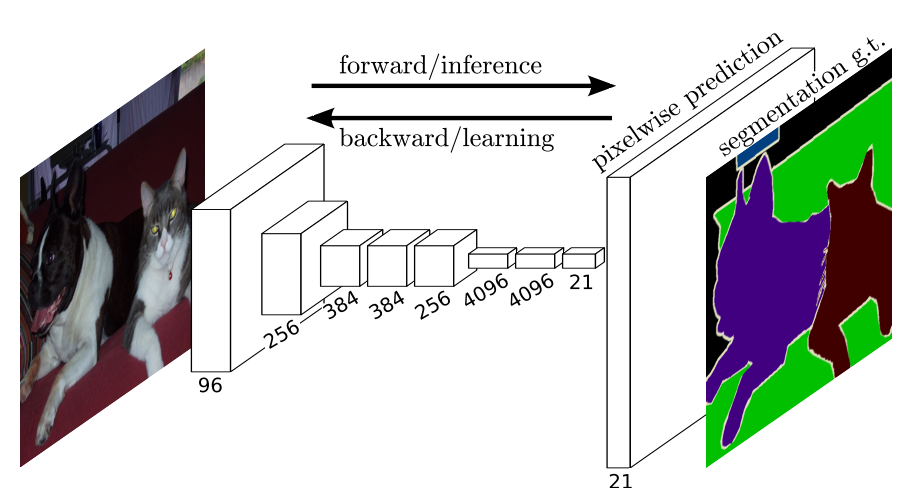
\includegraphics[width=\textwidth]{figures/FCN} \\
		\makebox[0.5\textwidth]{\tiny a. 全卷积网络[Long et al, CVPR 2015]} \\
		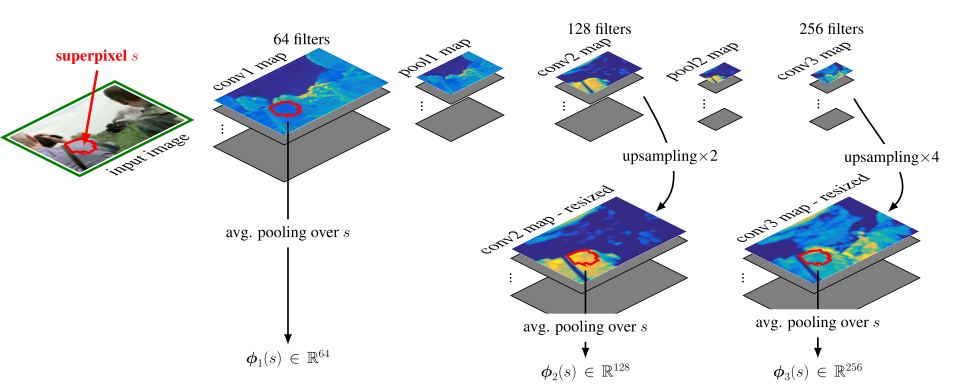
\includegraphics[width=\textwidth]{figures/zoom-out} \\
		\makebox[0.5\textwidth]{\tiny c. 卷积网络+高低层次特征融合[Mostajabi et al, CVPR 2015]}

		\column{.5\textwidth}
		\centering
		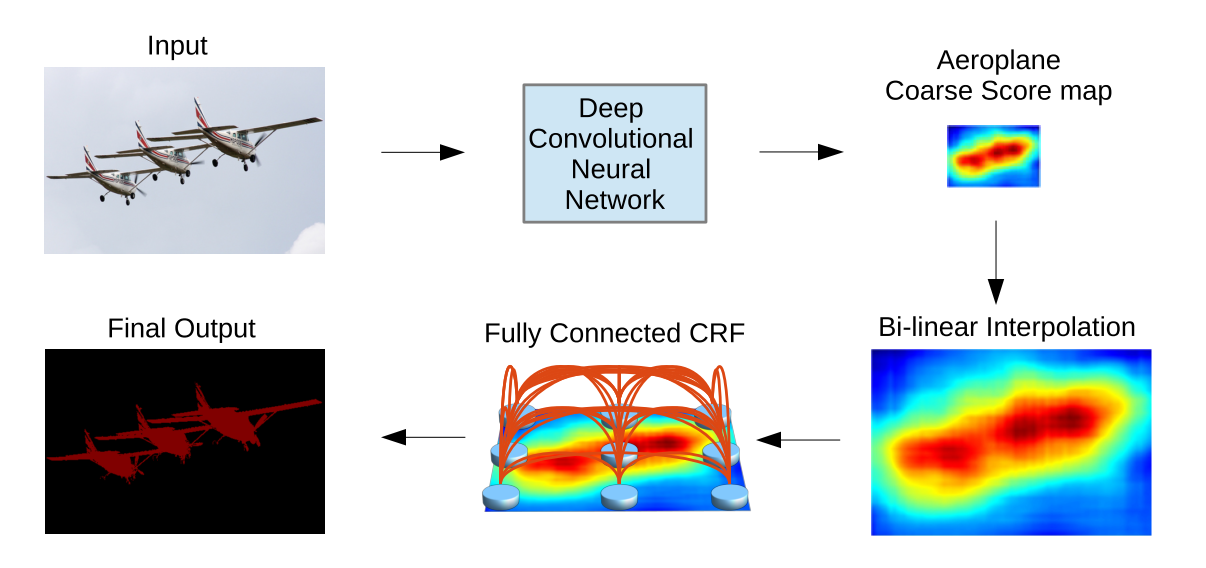
\includegraphics[width=\textwidth]{figures/Deeplab} \\
		\makebox[0.5\textwidth]{\tiny b. 全卷积网络+概率图模型[Chen et al, ICLR 2015]} \\
		\vspace{0.8em}
		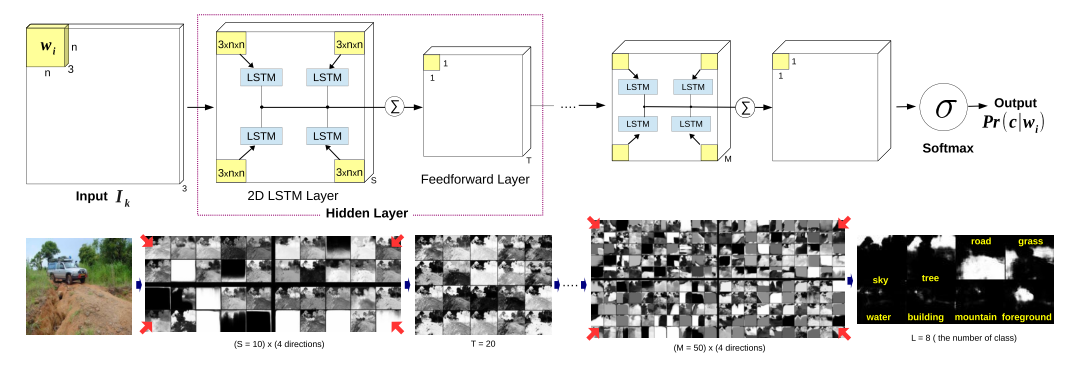
\includegraphics[width=\textwidth]{figures/LSTM} \\
		\makebox[0.5\textwidth]{\tiny d. 二维长短记忆网络[Byeon et al, CVPR, 2015]}
	\end{columns}
}
\subsection*{本文的工作}
\frame{
	\vspace{-0.6em}
	\begin{figure}[h]
		\centering
		\includegraphics[width=\textwidth]{image/illustration/networkstructure.pdf}
		\caption{网络整体结构图}
	\end{figure}
	\vspace{-1.2em}
	\begin{block}{目标与思路}
		\footnotesize
		\begin{itemize}
			\item 充分利用全卷积网络强大的特征学习能力
			\item 借助长短记忆网络对特征整体与局部建模的良好能力
			\item 使用随机梯度下降法进行端到端的训练
			\item 在主流数据集验证模型有效性
		\end{itemize}
	\end{block}
}


\newclearpage
\chapter{光声成像的理论基础}

\label{cha:sysu-thesis-contents-format-requirement}

\section{光声成像的波动方程}
假设$p(x,t)$为位于整个采集表面S上位置$x$的点在时刻$t$($t$≥0)的压力值。并且记位于表面S上位置$y$的点状声波探测器在观测时刻$t$获得的声波压力数据为函数$g(y,t)$,即$g(y,t):=p(y,t) \ for \ y\in S,t\geqslant0$。

于是我们得到一个波动方程:
\begin{equation} \label{201}
	\left\{
	\begin{aligned}
		& p_{tt}=c^2(x)\vartriangle _xp,\quad t\geqq0,x\in\mathbb{R}^3\\
		& p(x,0)=f(x),p_t(x,0)=0 \\
		& p|_s = g(y,t),\quad (y,t)\in S\times\mathbb{R}^+.
	\end{aligned}
	\right.
\end{equation}
其中,$f(x)$是声压的初始值。因此,光声成像的目标是使用传感器的测量数据$g(y,t)$,反推出上述波动方程$p(x,t)$在t=0处的初始值$f(x)$。

我们做如下记号:

定义1:我们使用$\mathcal{W}$表示正算子,即$\mathcal{W}:f(x)\to g(y,t)$,其中$f$与$g$的定义同上述波动方程。

如果成像介质是均匀的,即$c(x)$等于一个常数,我们假设该常数在适当的单位下等于1。此时,波动方程为:
\begin{equation} \label{202}
	\left\{
	\begin{aligned}
		& p_{tt}=\vartriangle _xp \quad \quad \ \ t\geqq0,x\in\mathbb{R}^3\\
		& p(x,0)=f(x),p_t(x,0)=0\\
		& p|_s = g(y,t),\quad (y,t)\in S\times\mathbb{R}^+.
	\end{aligned}
	\right.
\end{equation}


此时,根据$Poisson\ Kirchhoff$公式,我们能得到上述波动方程的解为:
\begin{equation} \label{203}
\begin{aligned}
p(x,t)=a\cfrac{\partial}{\partial t}(t(Rf)(x,t)).
\end{aligned}
\end{equation}
其中$(Rf)(x,r):=\cfrac{1}{4\pi}\int_{|y|=1} f(x+ry)\, dA(y)$是作用于函数$f(x)$的球面平均算子,$dA$是$\mathbb{R}^3$单位球面上的标准面积元,$a$为常数。

从上述公式可以得知,$p(x,t)$由函数$f$的球面平均值$(Rf)(x,t)$唯一决定。我们将这个这个球面平均算子作用在$f$上的映射$R:f→R$f记为$\mathcal{M}$,即:
\begin{equation} \label{204}
	\begin{aligned}
		\mathcal{M}f(x,t):=\cfrac{1}{4\pi}\int_{|y|=1} f(x+ry)\, dA(y),\quad x\in S,t\geqq0.
	\end{aligned}
\end{equation}
因此,在成像介质是均匀的情况下,我们可以选择使用$\mathcal{M}$来代替$p(x,t)$进行研究。

\section{光声成像的重建算法}
对于成像介质是均匀介质的情况(此时$c(x)$为常数),有上面的讨论可得,光声成像的图像重建等效于求解球面均值变换$\mathcal{M}$的逆。
下面介绍几种常见的光声成像重建方法:

\subsection{幂级数解法}
将$f$和$g$进行傅里叶分解后,即

\begin{equation} \label{205}
	\begin{aligned}
		f(x)=\sum_{-\infty}^{+\infty} f_k(\rho )e^{ik\varphi},\quad x=(\rho cos(\varphi),\rho sin(\varphi)).
	\end{aligned}
\end{equation}

\begin{equation} \label{206}
	\begin{aligned}
		g(y(\theta),r)=\sum_{-\infty}^{+\infty}g_k(r)e^{ik\theta},\quad y=(Rcos(\theta),Rsin(\theta)).
	\end{aligned}
\end{equation}

将其代入到公式(\ref{203})中,由等式两边系数相等可得:

\begin{equation} \label{207}
	\begin{aligned}
		f_k(\rho)=\mathcal{H}_m(\cfrac{1}{J_k(\lambda|R|)}\mathcal{H}_0\big[ \cfrac{g_k(r)}{2\pi r}\big]).
	\end{aligned}
\end{equation}

其中$(\mathcal{H}_mu)(s)=2\pi \int_{0}^{\infty}u(t)J_m(st)t dt$为Hankel变换,$J_m(t)$为贝塞尔函数。

应该注意的是,幂级数解法依赖于在球面几何中成立的变量分离,因此这种方法仅在球面上成立。


\subsection{特征函数展开法}

设$\lambda_m$和$u_m(x)$为封闭曲面S内部Ω的狄利克雷-拉普拉斯算子$−\vartriangle$的特征值和特征函数的正交基,满足:

\begin{equation} \label{208}
\left\{
\begin{aligned}
	& \vartriangle u_m(x)+\lambda_m^2u_m(x)=0,\quad x\in \Omega,\Omega\subseteq \mathbb{R}^n\\
	& u_m(x)=0,\quad \quad \quad \qquad \qquad x\in S\\
	& ||u_m||_2^2\equiv\int_{\Omega}|u_m(x)|^2dx=1.
\end{aligned}
\right.
\end{equation}

可解得:

\begin{equation} \label{209}
	\begin{aligned}
		u_m(x)=\int_{S}\Phi_{\lambda_m}(|x-y|)\cfrac{\partial}{\partial n}u_m(y)ds(y),\quad x\in\Omega.
	\end{aligned}
\end{equation}

其中$\Phi_{\lambda_m}(|x-y|)$是亥姆霍兹方程的自由空间格林函数,$n$是$S$的外法向量。

函数$f(x)$可以展开成级数:

\begin{equation} \label{210}
	\begin{aligned}
		f(x)=\sum_{m=0}^{\infty}\alpha_mu_m(x),\quad where\ \alpha_m=\int_{\Omega}u_m(x)f(x)dx.
	\end{aligned}
\end{equation}

如果将表示形式 ( \ref{209} ) 替换为表示形式( \ref{210} )并交换积分顺序,则可以得到$\alpha_m$。

\begin{equation} \label{211}
	\begin{aligned}
		& \alpha_m=\int_{\Omega}u_m(x)f(x)dx=\int_S I(y,\lambda_m)\cfrac{\partial}{\partial n}u_m(y)dA(x),\\
		& where\\
		& I(y,\lambda)=\int_{\Omega}\Phi_{\lambda}(|x-y|)f(x)dx=\int_0^{diam\Omega}g(y,r)\Phi_{\lambda}(r)dr.
	\end{aligned}
\end{equation}

将$\alpha_m$代入级数(\ref{210})就能得到重建公式$f(x)$。

\newclearpage
\chapter{Transformer的理论基础}


\label{cha:sysu-thesis-latex-install-guide}
\section{transformer的简介}

Transformer是最早在自然语言处理领域提出并逐渐被广泛运用于其他领域的神经网络模型。Transformer的出现在性能上超越了很多传统的自然语言处理模型如RNN、LSTM等。并且Transformer还具有突破了并行计算的限制、更具可解释性等优点。

在最开始的使用中,transformer包括encoding(编码器)和decoding(解码器)两个部分。其神经网络的结构如图\ref{img301}所示:

\begin{figure}[h]
	\centering
	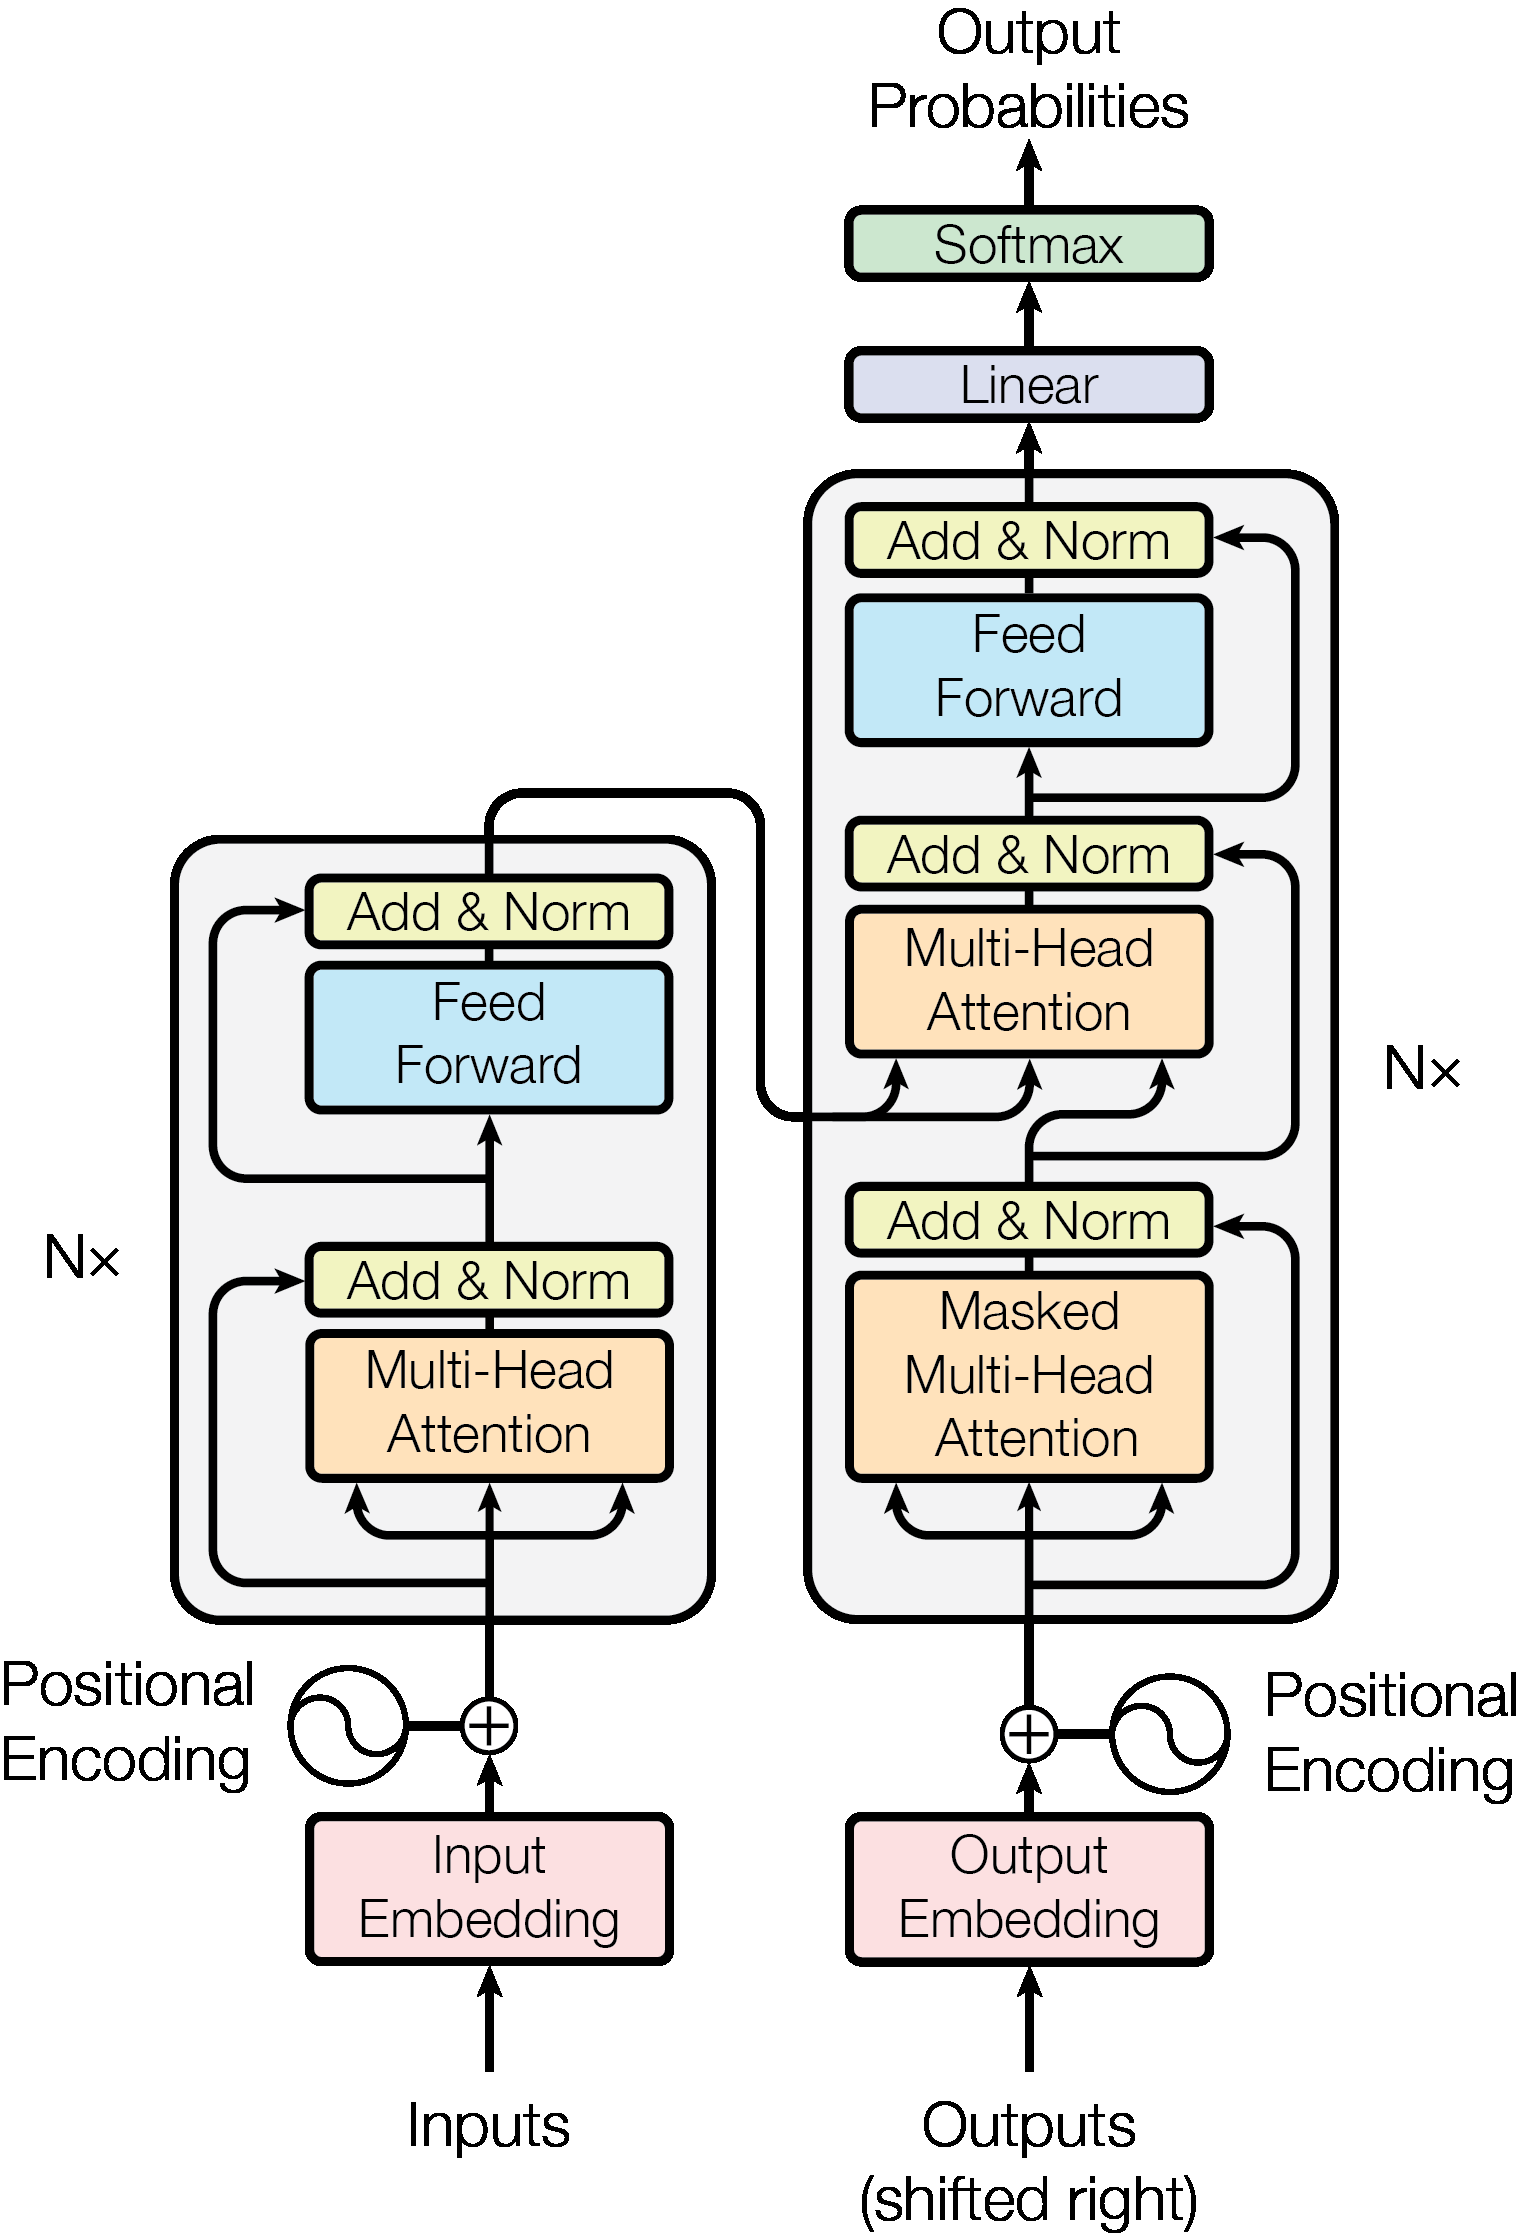
\includegraphics[width=0.4\columnwidth]{image/chap03/img301.png}
	\caption{"Attention Is All You Need"中的Transformer模型\cite{vaswani2017attention}}
	\label{img301}
\end{figure}

\section{自注意力机制}
\subsection{注意力机制的原理}
注意力机制是Transformer的核心机制。自注意力机制的提出是对人类获取外界信息的机制的一种抽象。当我们观察外界信息,并不是对外界的所有信息“全盘吸收”,而是会无意识地忽略某些“不重要”的信息,从而能提高对外界信息的吸收效率。我们用一个机器翻译的任务来阐述注意力机制的原理。

\begin{figure}[h]
	\begin{minipage}[t]{0.5\linewidth}
		\centering
		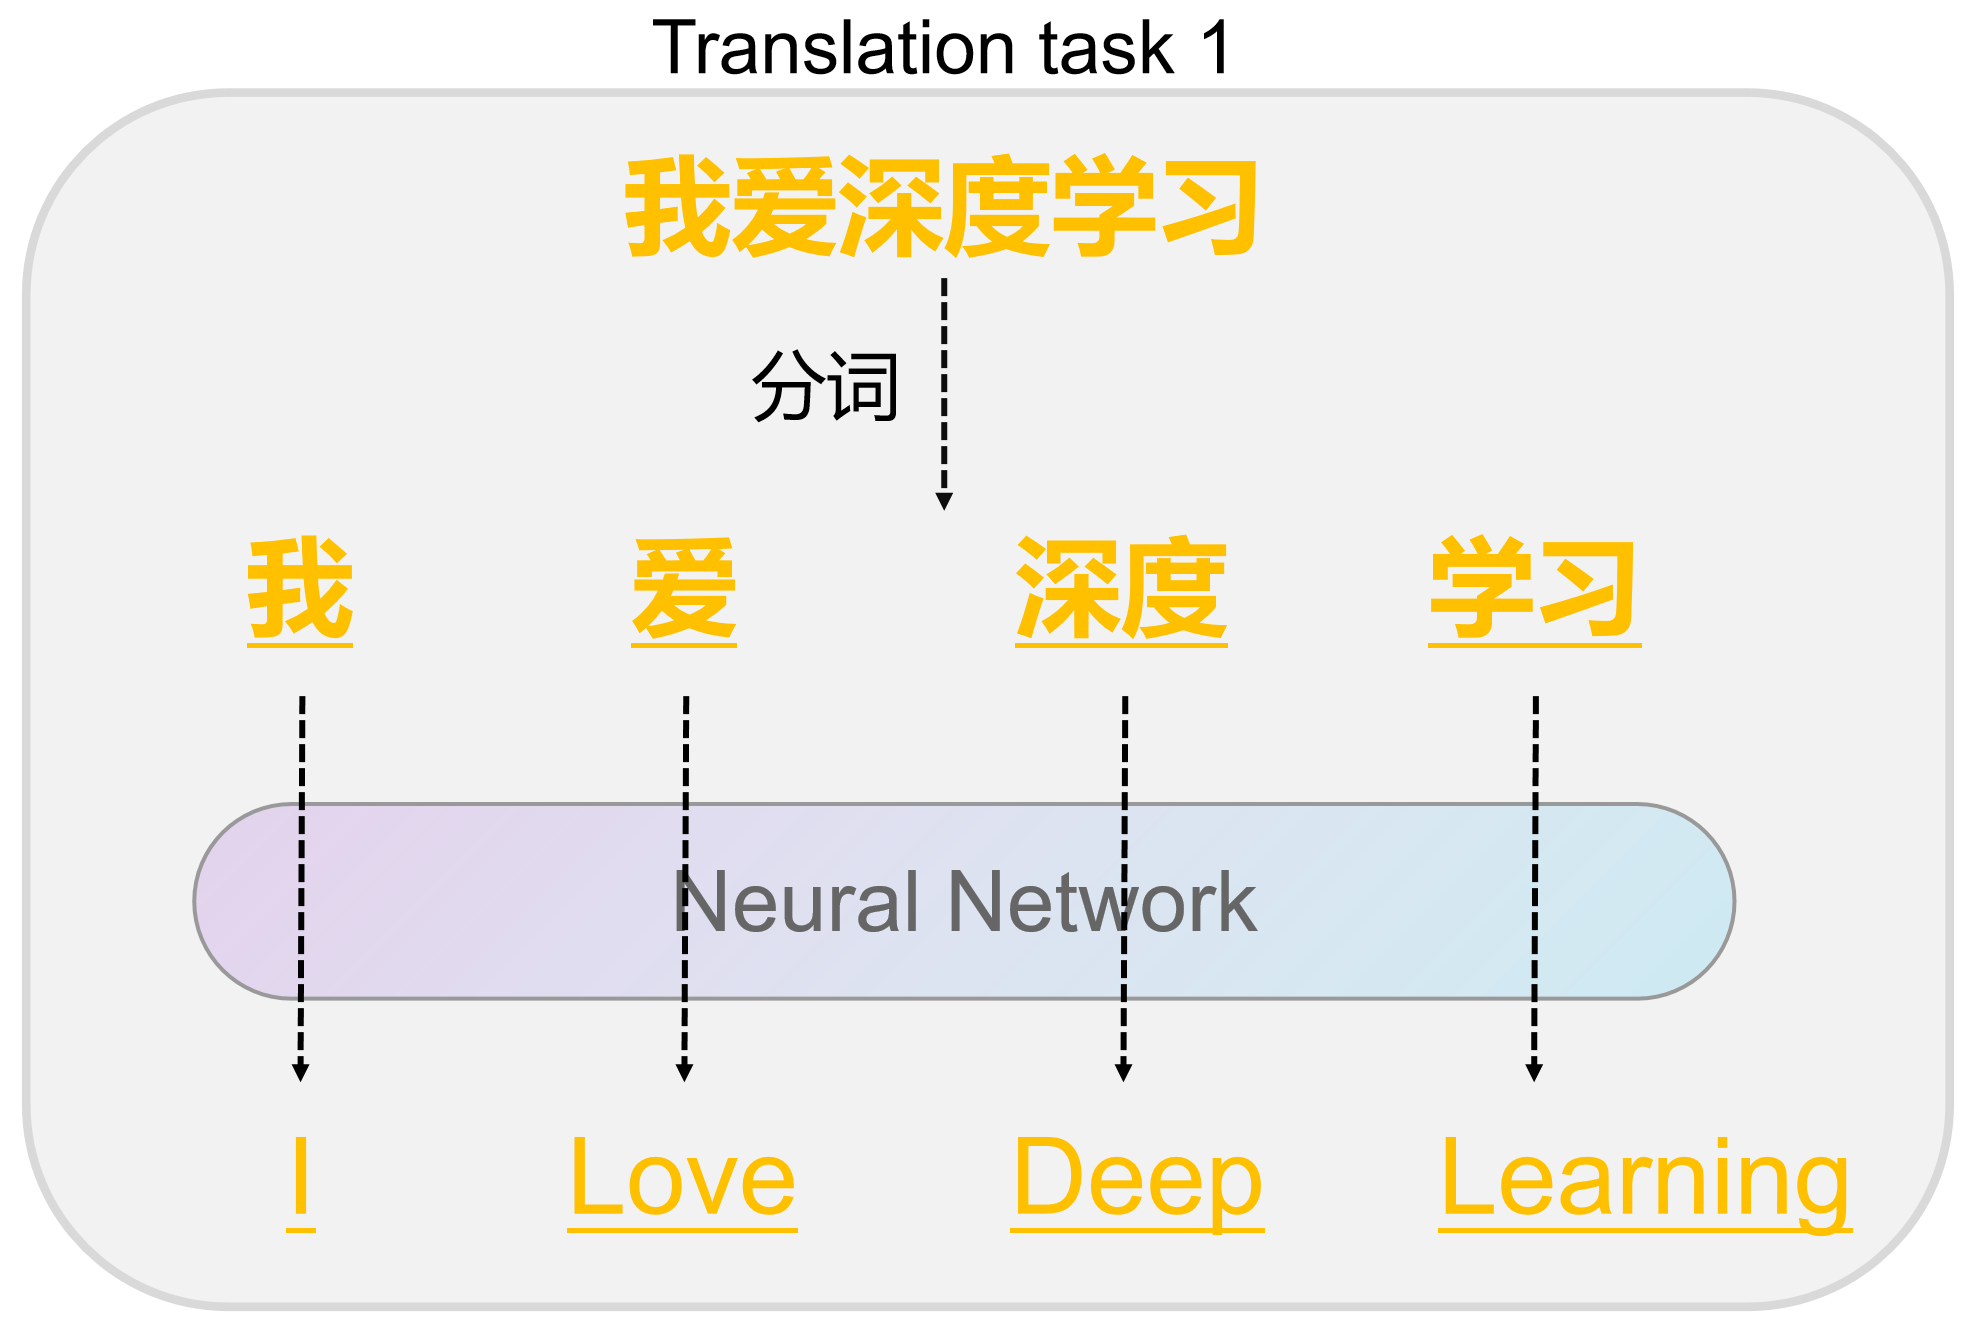
\includegraphics[scale=0.25]{image/chap03/img302.png}
		\caption{翻译任务1}
		\label{img302}
	\end{minipage}%
	\begin{minipage}[t]{0.5\linewidth}
		\centering
		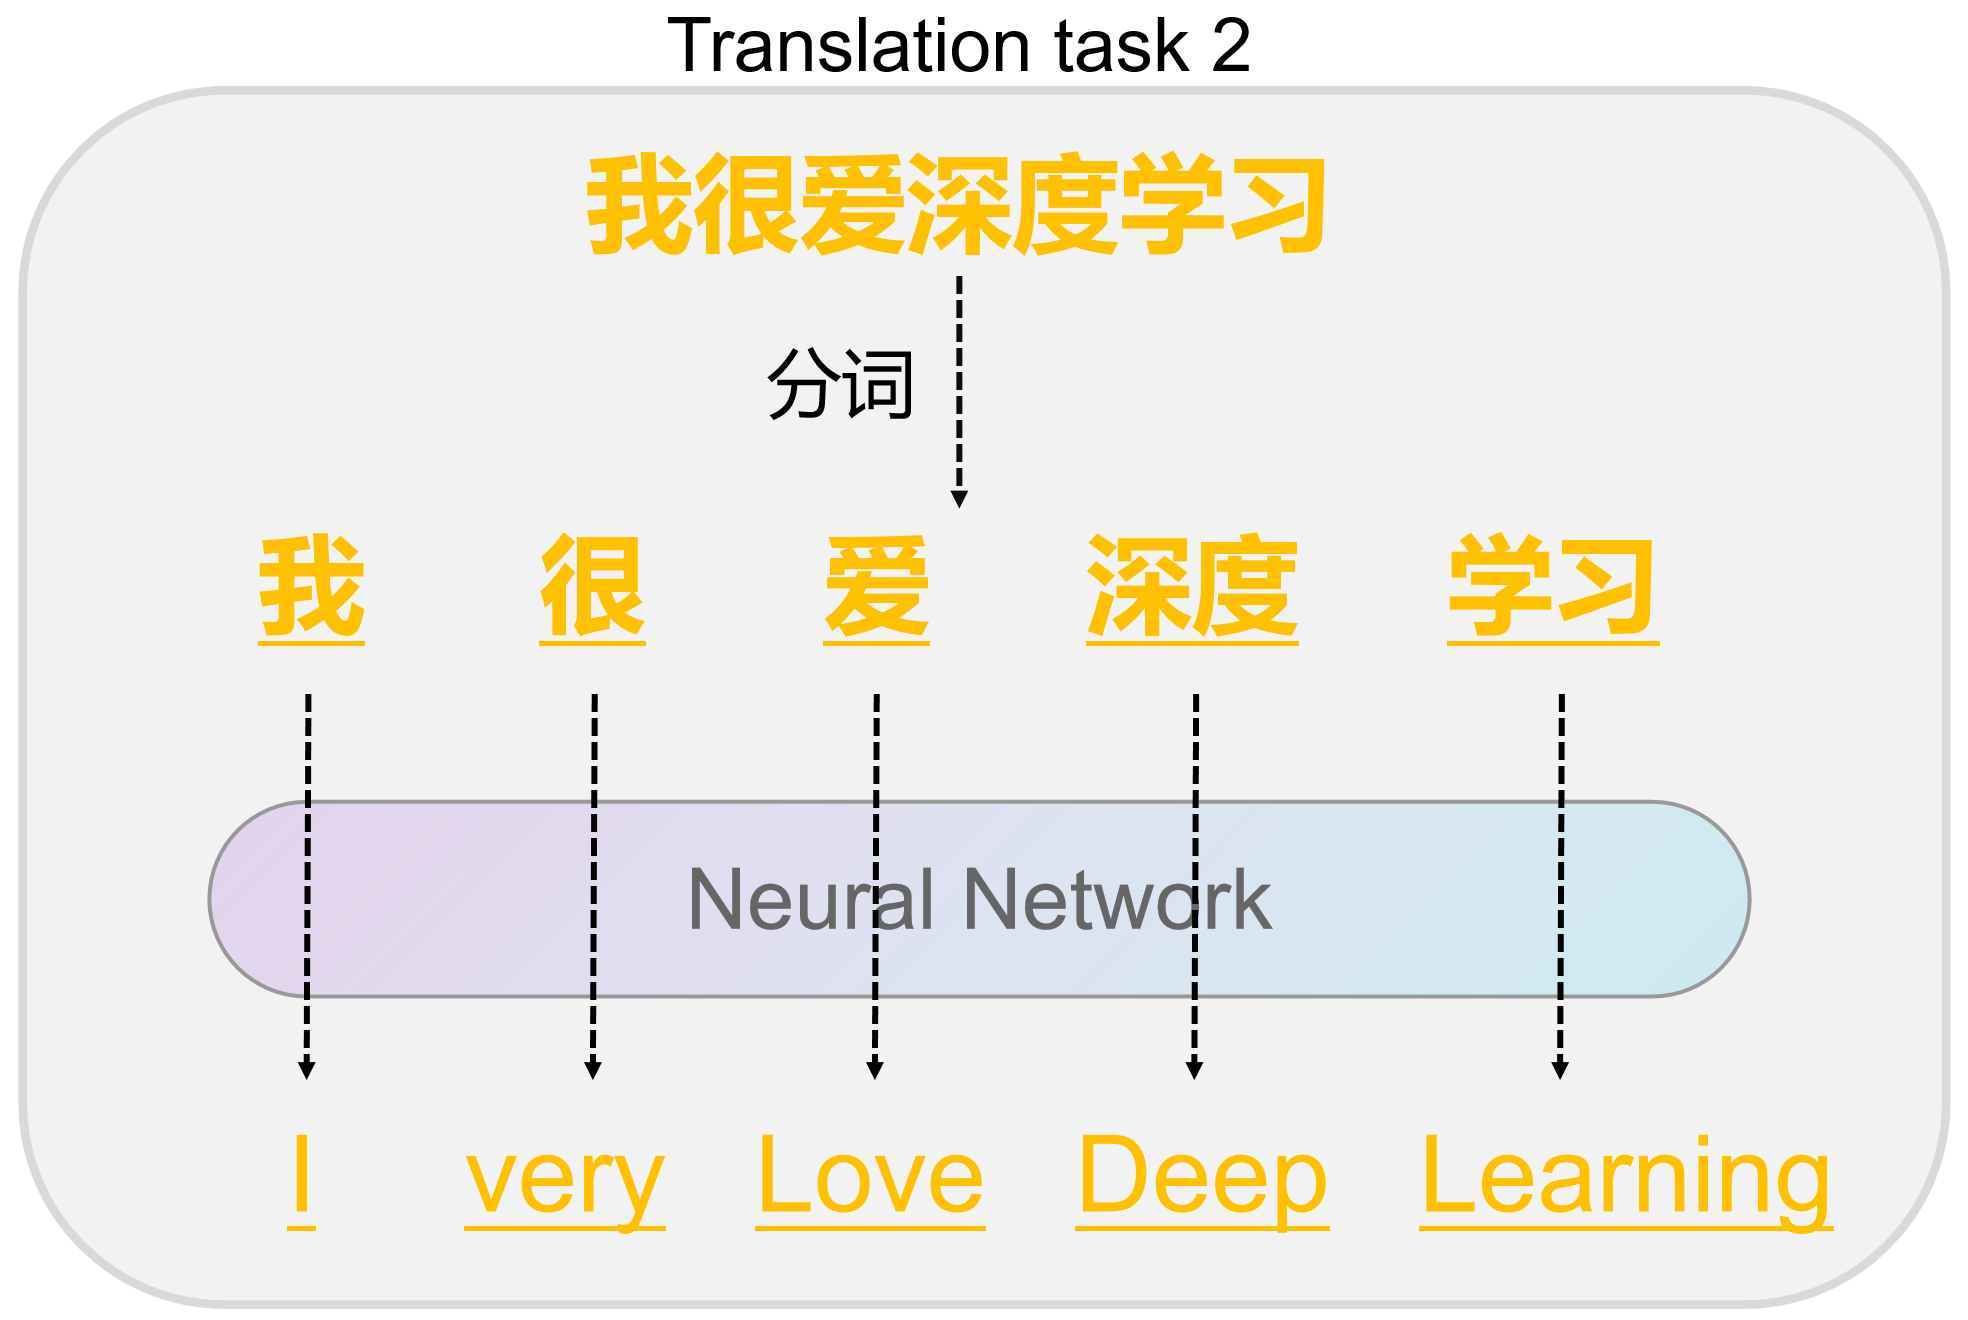
\includegraphics[scale=0.25]{image/chap03/img303.png}
		\caption{翻译任务2}
		\label{img303}
	\end{minipage}
\end{figure}

假设我们要使用神经网络来完成中译英的机器翻译任务。如果完全不考虑整个句子的上下文信息,那么机器翻译其实就是训练神经网络,使其能将特定的中文字符映射到特定的英文字符,这时只需采用最简单的Mlp神经网络就能实现这种功能。这种做法在某些机器翻译任务中是可行的,如图\ref{img302}。但在大多数的机器翻译任务中,这种直接映射的做法会导致语法上的错误或语义上的歧义,如图\ref{img303}的机器翻译任务。

这时,在翻译单个词时,通过结合上下文信息再进行翻译就十分重要了。而Transformer中的注意力机制就能很好地实现上下文信息的结合。首先在进行机器翻译的任务之前,都会对翻译的单词进行“编码”使其能被计算机运算与处理。比如将四字句子“我”“很”“爱”“深度”“学习”编码成五个向量$x_1,x_2,x_3,x_4,x_5$。并记$X=[x_1,x_2,x_3,x_4,x_5]$代表整个句子,即如图\ref{img304}所示.

\begin{figure}[h]
	\centering
	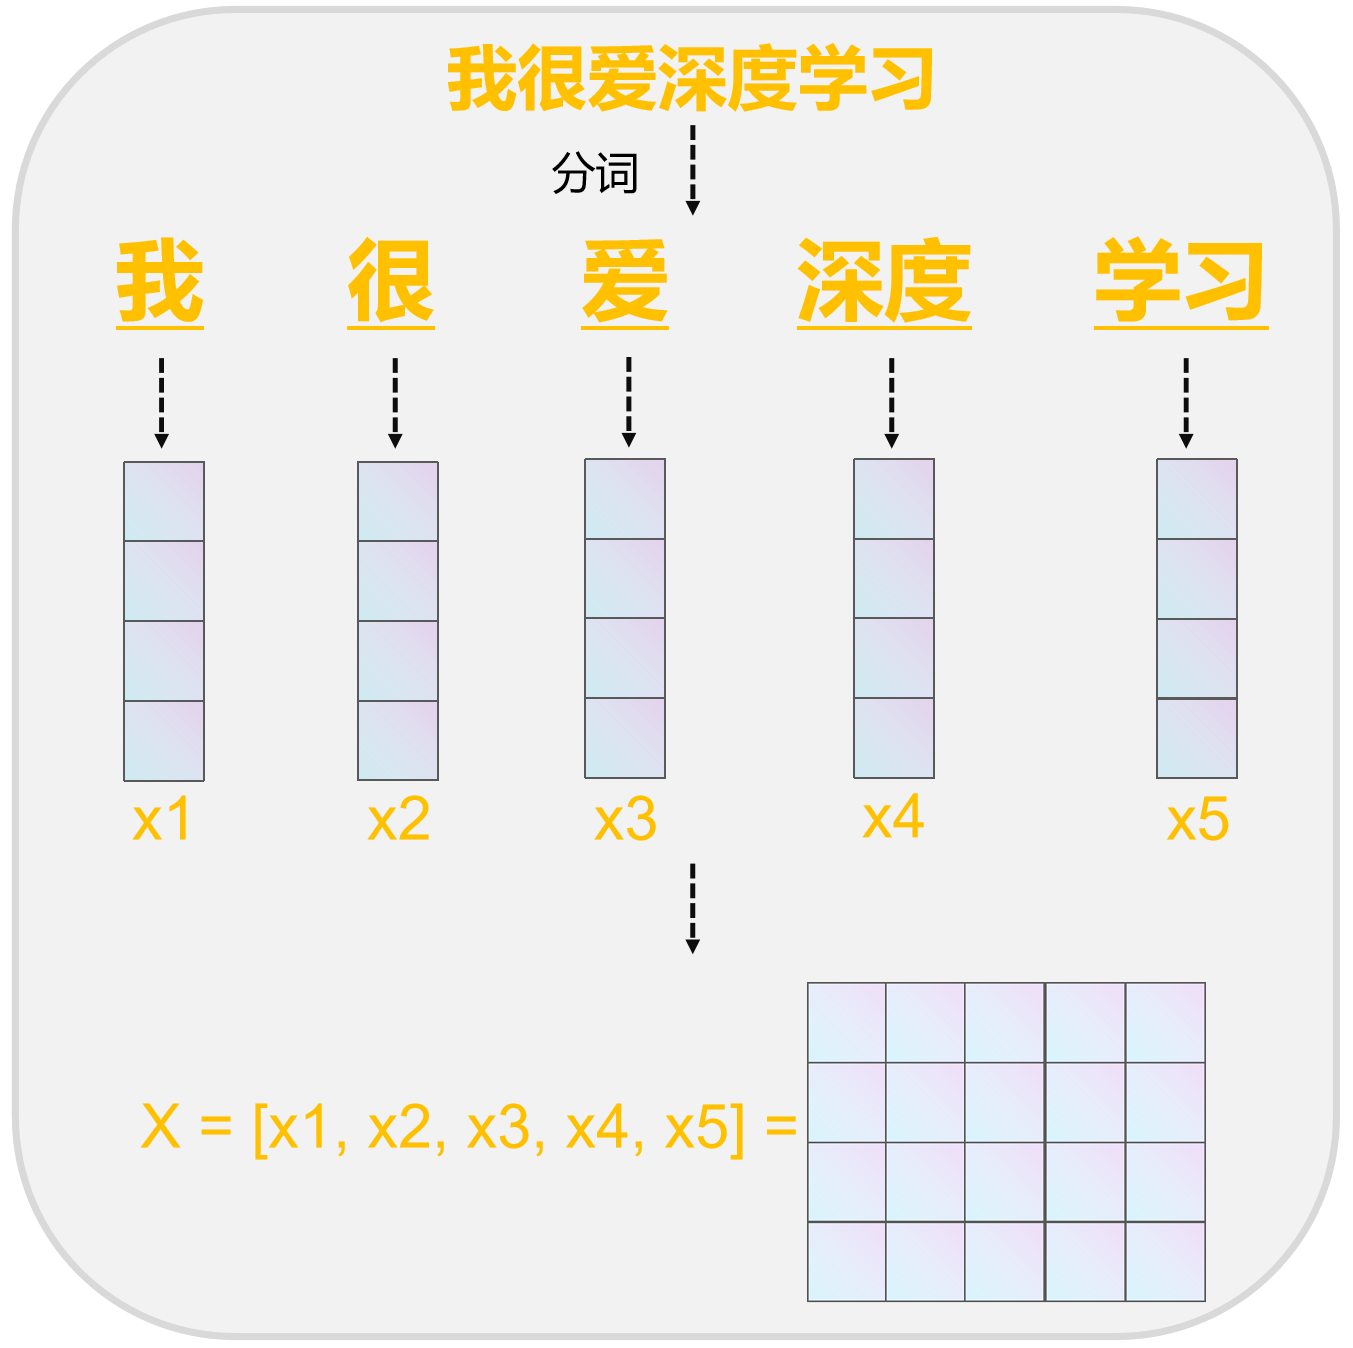
\includegraphics[width=0.4\columnwidth]{image/chap03/img304.png}
	\caption{自然语言编码过程}
	\label{img304}
\end{figure}

 在翻译词“很”的时候,我们想知道所在句子中的其他词所提供的信息量的程度。我们需要找到一个值域为$[ 0, 1]$的注意力打分函数$F$,来衡量这种提供信息的权重。即若我们输入$F($“很”,“我”$)=$$F(x_2,x_1)=\omega_{21}$,所得到的$\omega_{21}$代表在翻译“很”字时,“我”字所提供信息的权重。以此类推,我们可以得到各个字在翻译“很”字时提供的信息权重$\omega_{21},\omega_{22},\omega_{23},\omega_{24},\omega_{25}$,即:

\begin{equation} \label{301}
\left\{
\begin{array}{l}
	F(\vec{x_2},\vec{x_1})=\omega_{21}\\
	F(\vec{x_2},\vec{x_2})=\omega_{22}\\
	\qquad \qquad \ \ \vdots\\
	F(\vec{x_2},\vec{x_5})=\omega_{25}
\end{array}
\right.
\end{equation}

\begin{figure}[h]
	\begin{minipage}[t]{0.5\linewidth}
		\centering
		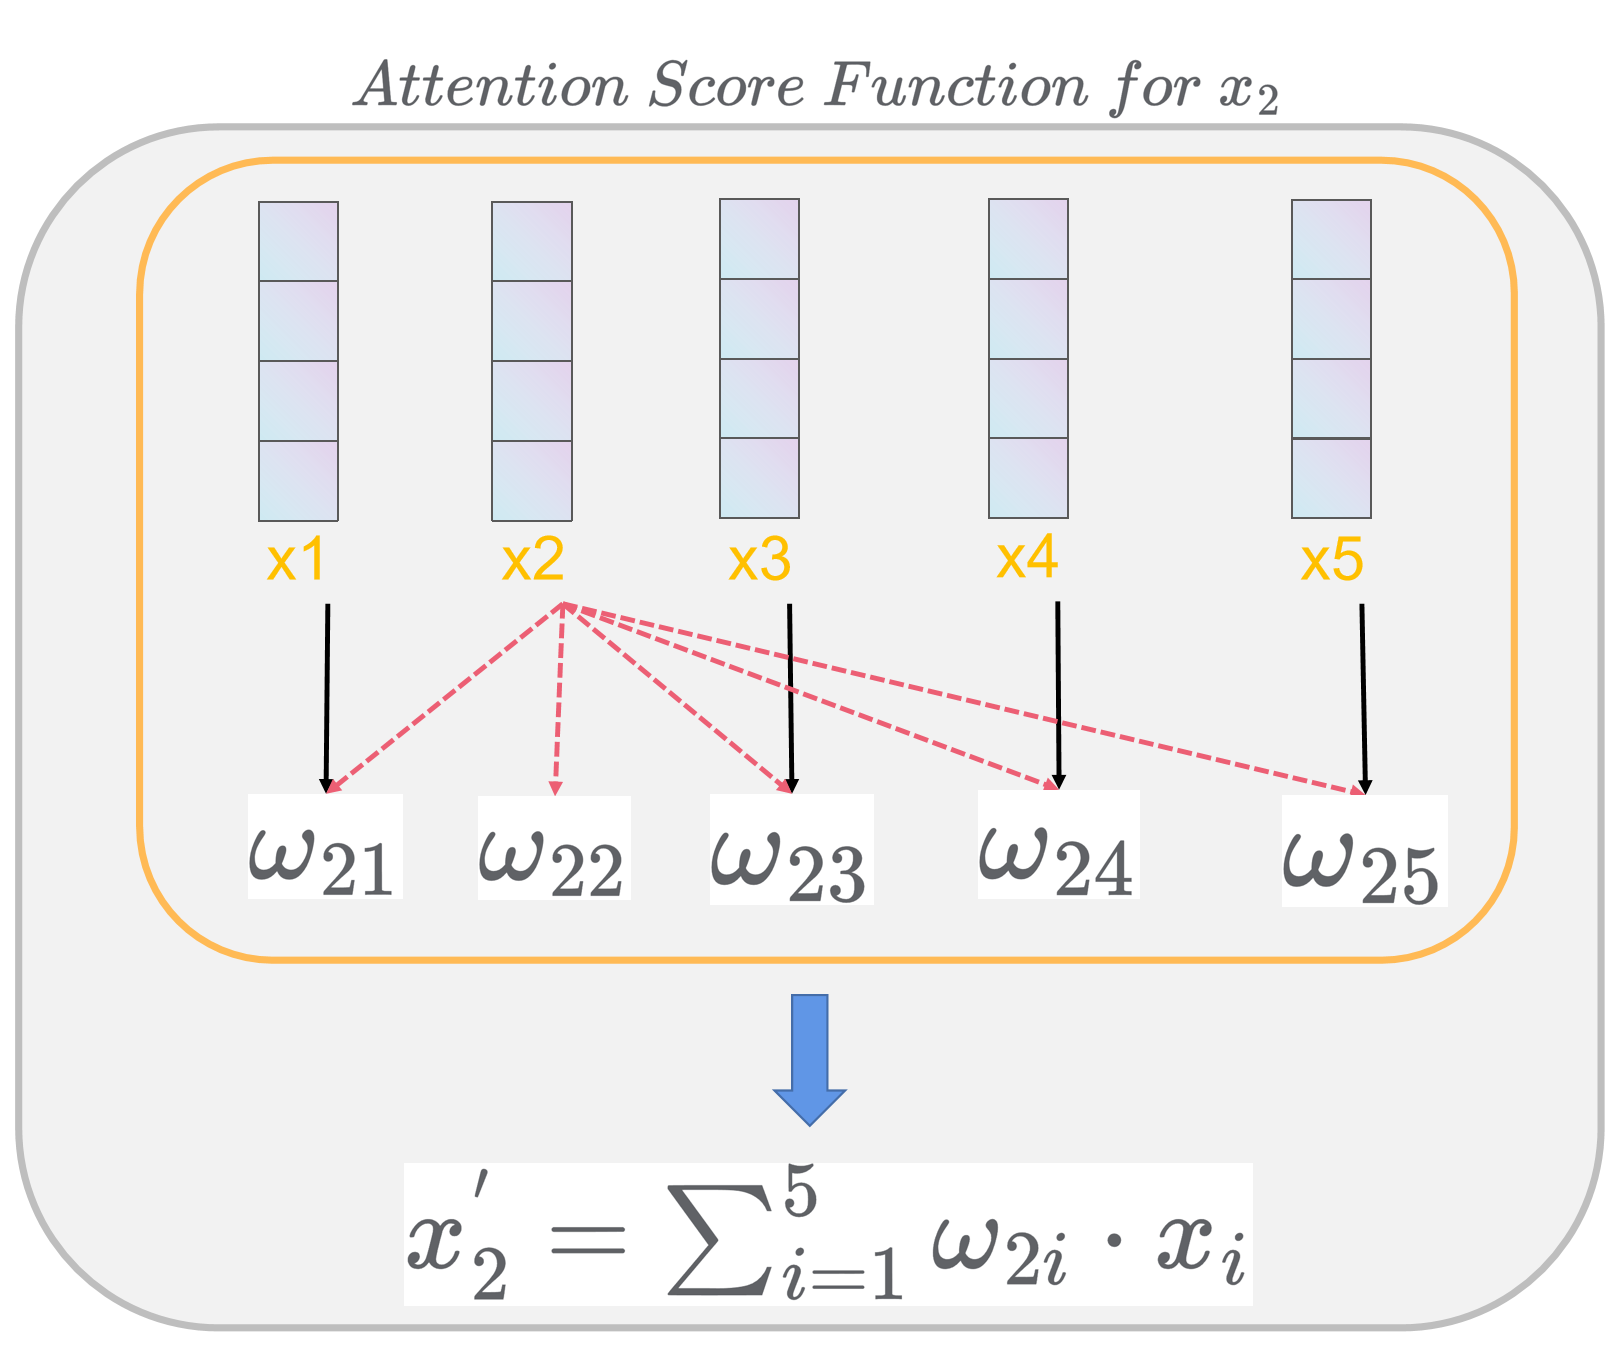
\includegraphics[scale=0.25]{image/chap03/img305.png}
		\caption{注意力机制的原理}
		\label{img305}
	\end{minipage}%
	\begin{minipage}[t]{0.5\linewidth}
		\centering
		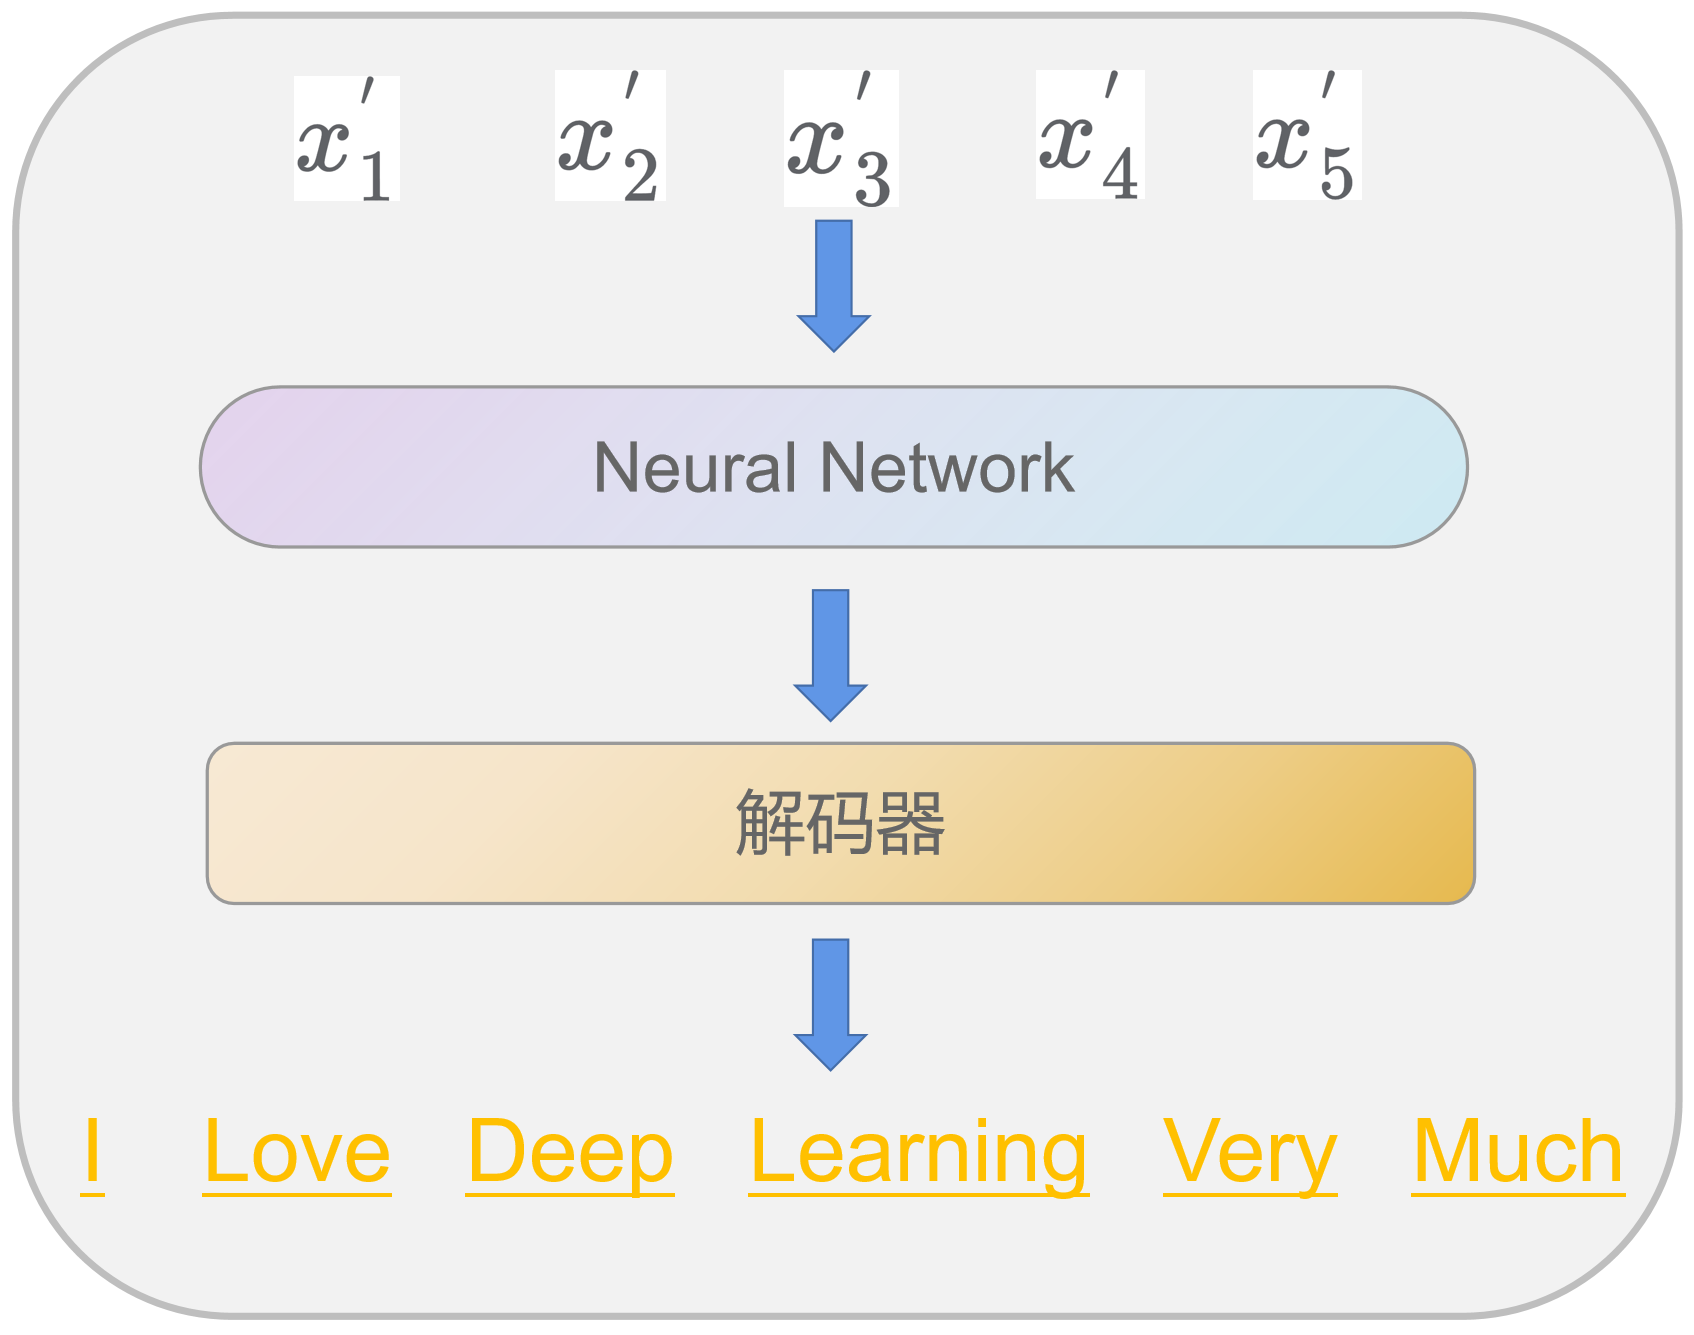
\includegraphics[scale=0.25]{image/chap03/img306.png}
		\caption{自然语言解码过程}
		\label{img306}
	\end{minipage}
\end{figure}

这时根据注意力权重进行加权求和得到的$x_2^{'} = \omega_{21}x_{1}+\omega_{22}x_{2}+\omega_{23}x_{3}+\omega_{24}x_{4}+\omega_{25}x_{5}$就能代表结合了上下文信息后的“很”字,如图\ref{img305}。同样的步骤,我们能得到结合了全局信息的$x_1^{'},…,x_5^{'}$,将其作为神经网络的输入,就能得到考虑了上下文信息的翻译,如图\ref{img306}。

机器翻译的Transformer模型就是上述的三个步骤的相互组合,如图\ref{img307}。

\begin{figure}[h]
	\centering
	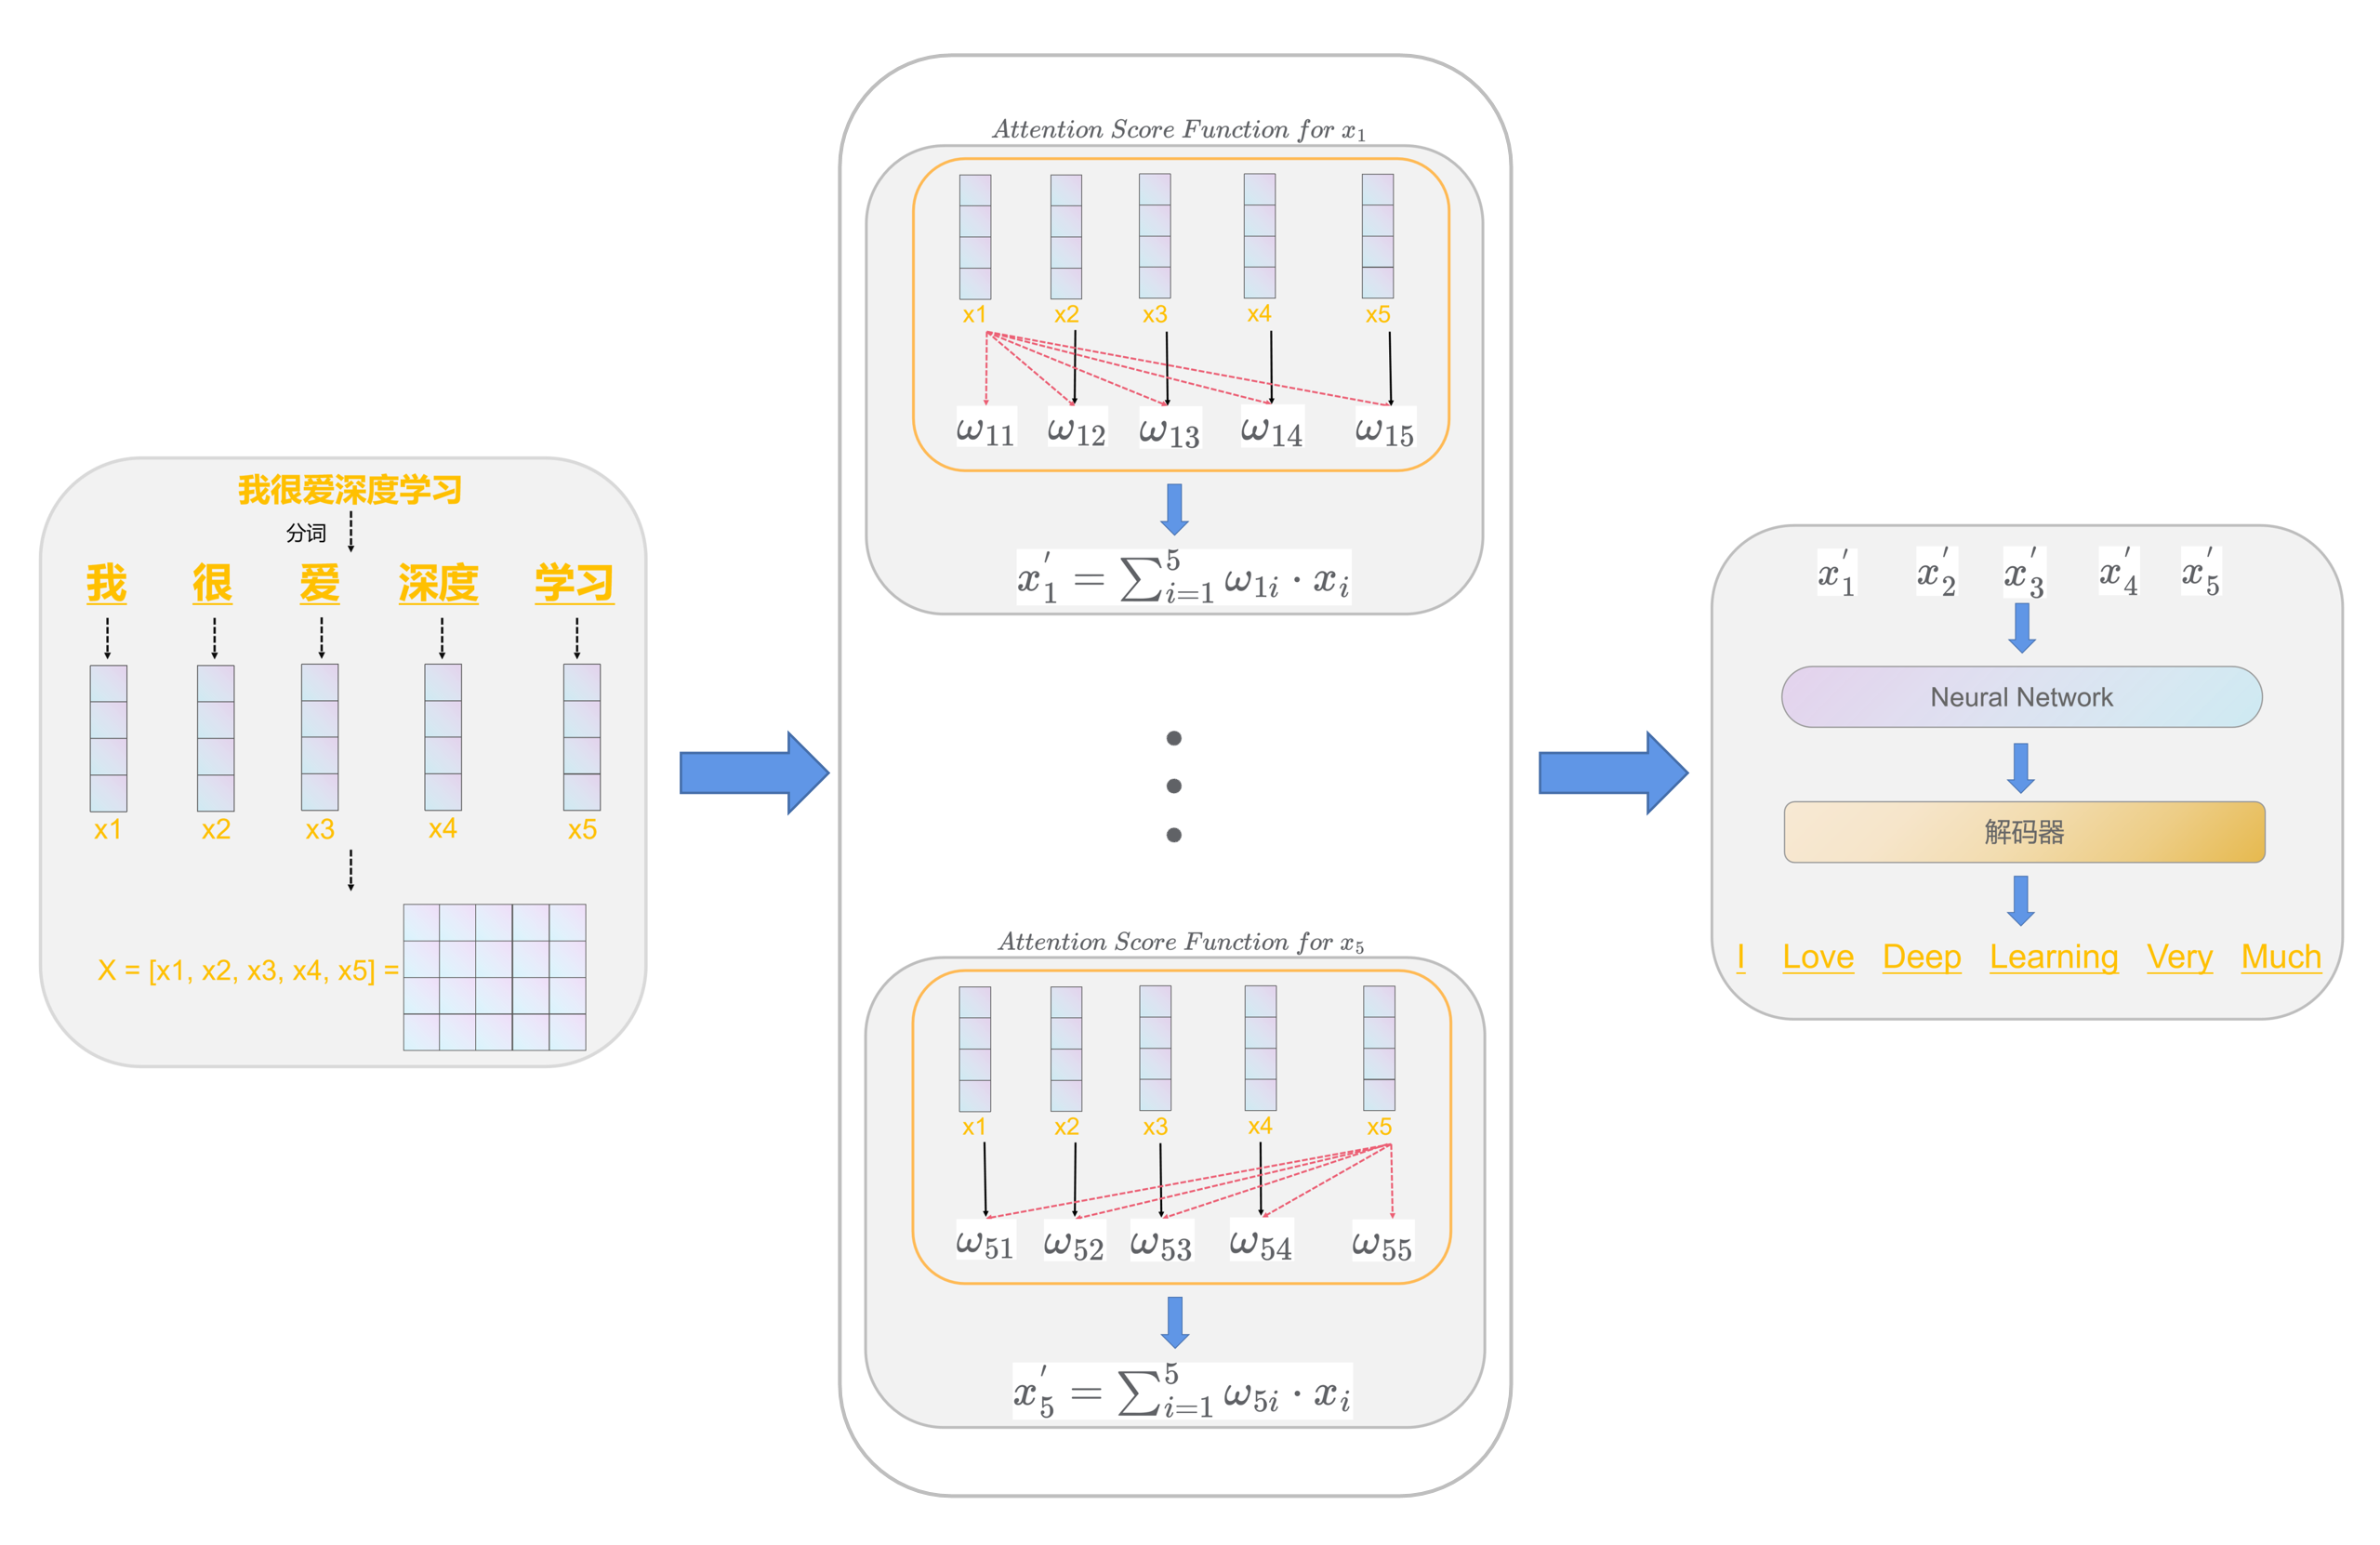
\includegraphics[width=0.9\columnwidth]{image/chap03/img307.png}
	\caption{运用注意力机制的机器翻译过程}
	\label{img307}
\end{figure}



\subsection{自注意力机制的实现}

自注意力机制的运算实现主要分成四个部分:

\subsubsection{将$X$经过三个线性变换后得到$Q,K,V$}

将多个研究对象进行编码后得到的的向量$x_1,\cdots ,x_n$(在如图\ref{img303}所示的任务中,$x_1,\cdots ,x_5$分别代表“我”“很”“爱”“深度”“学习”五个单词),将其按行排列而成的矩阵记为$X$,如图\ref{img308}左边。$X$矩阵与定义三个线性变换矩阵$W_q,W_k,W_v$相乘得到三个矩阵$Q,K,V$。得到的$Q,K,V$的各行元素各代表$X$矩阵中的一个向量。

其中$W_q,W_k,W_v$为可学习的参数,这一步的目的是为了使注意力打分函数成为可学习的函数。

\begin{figure}[h]
	\centering
	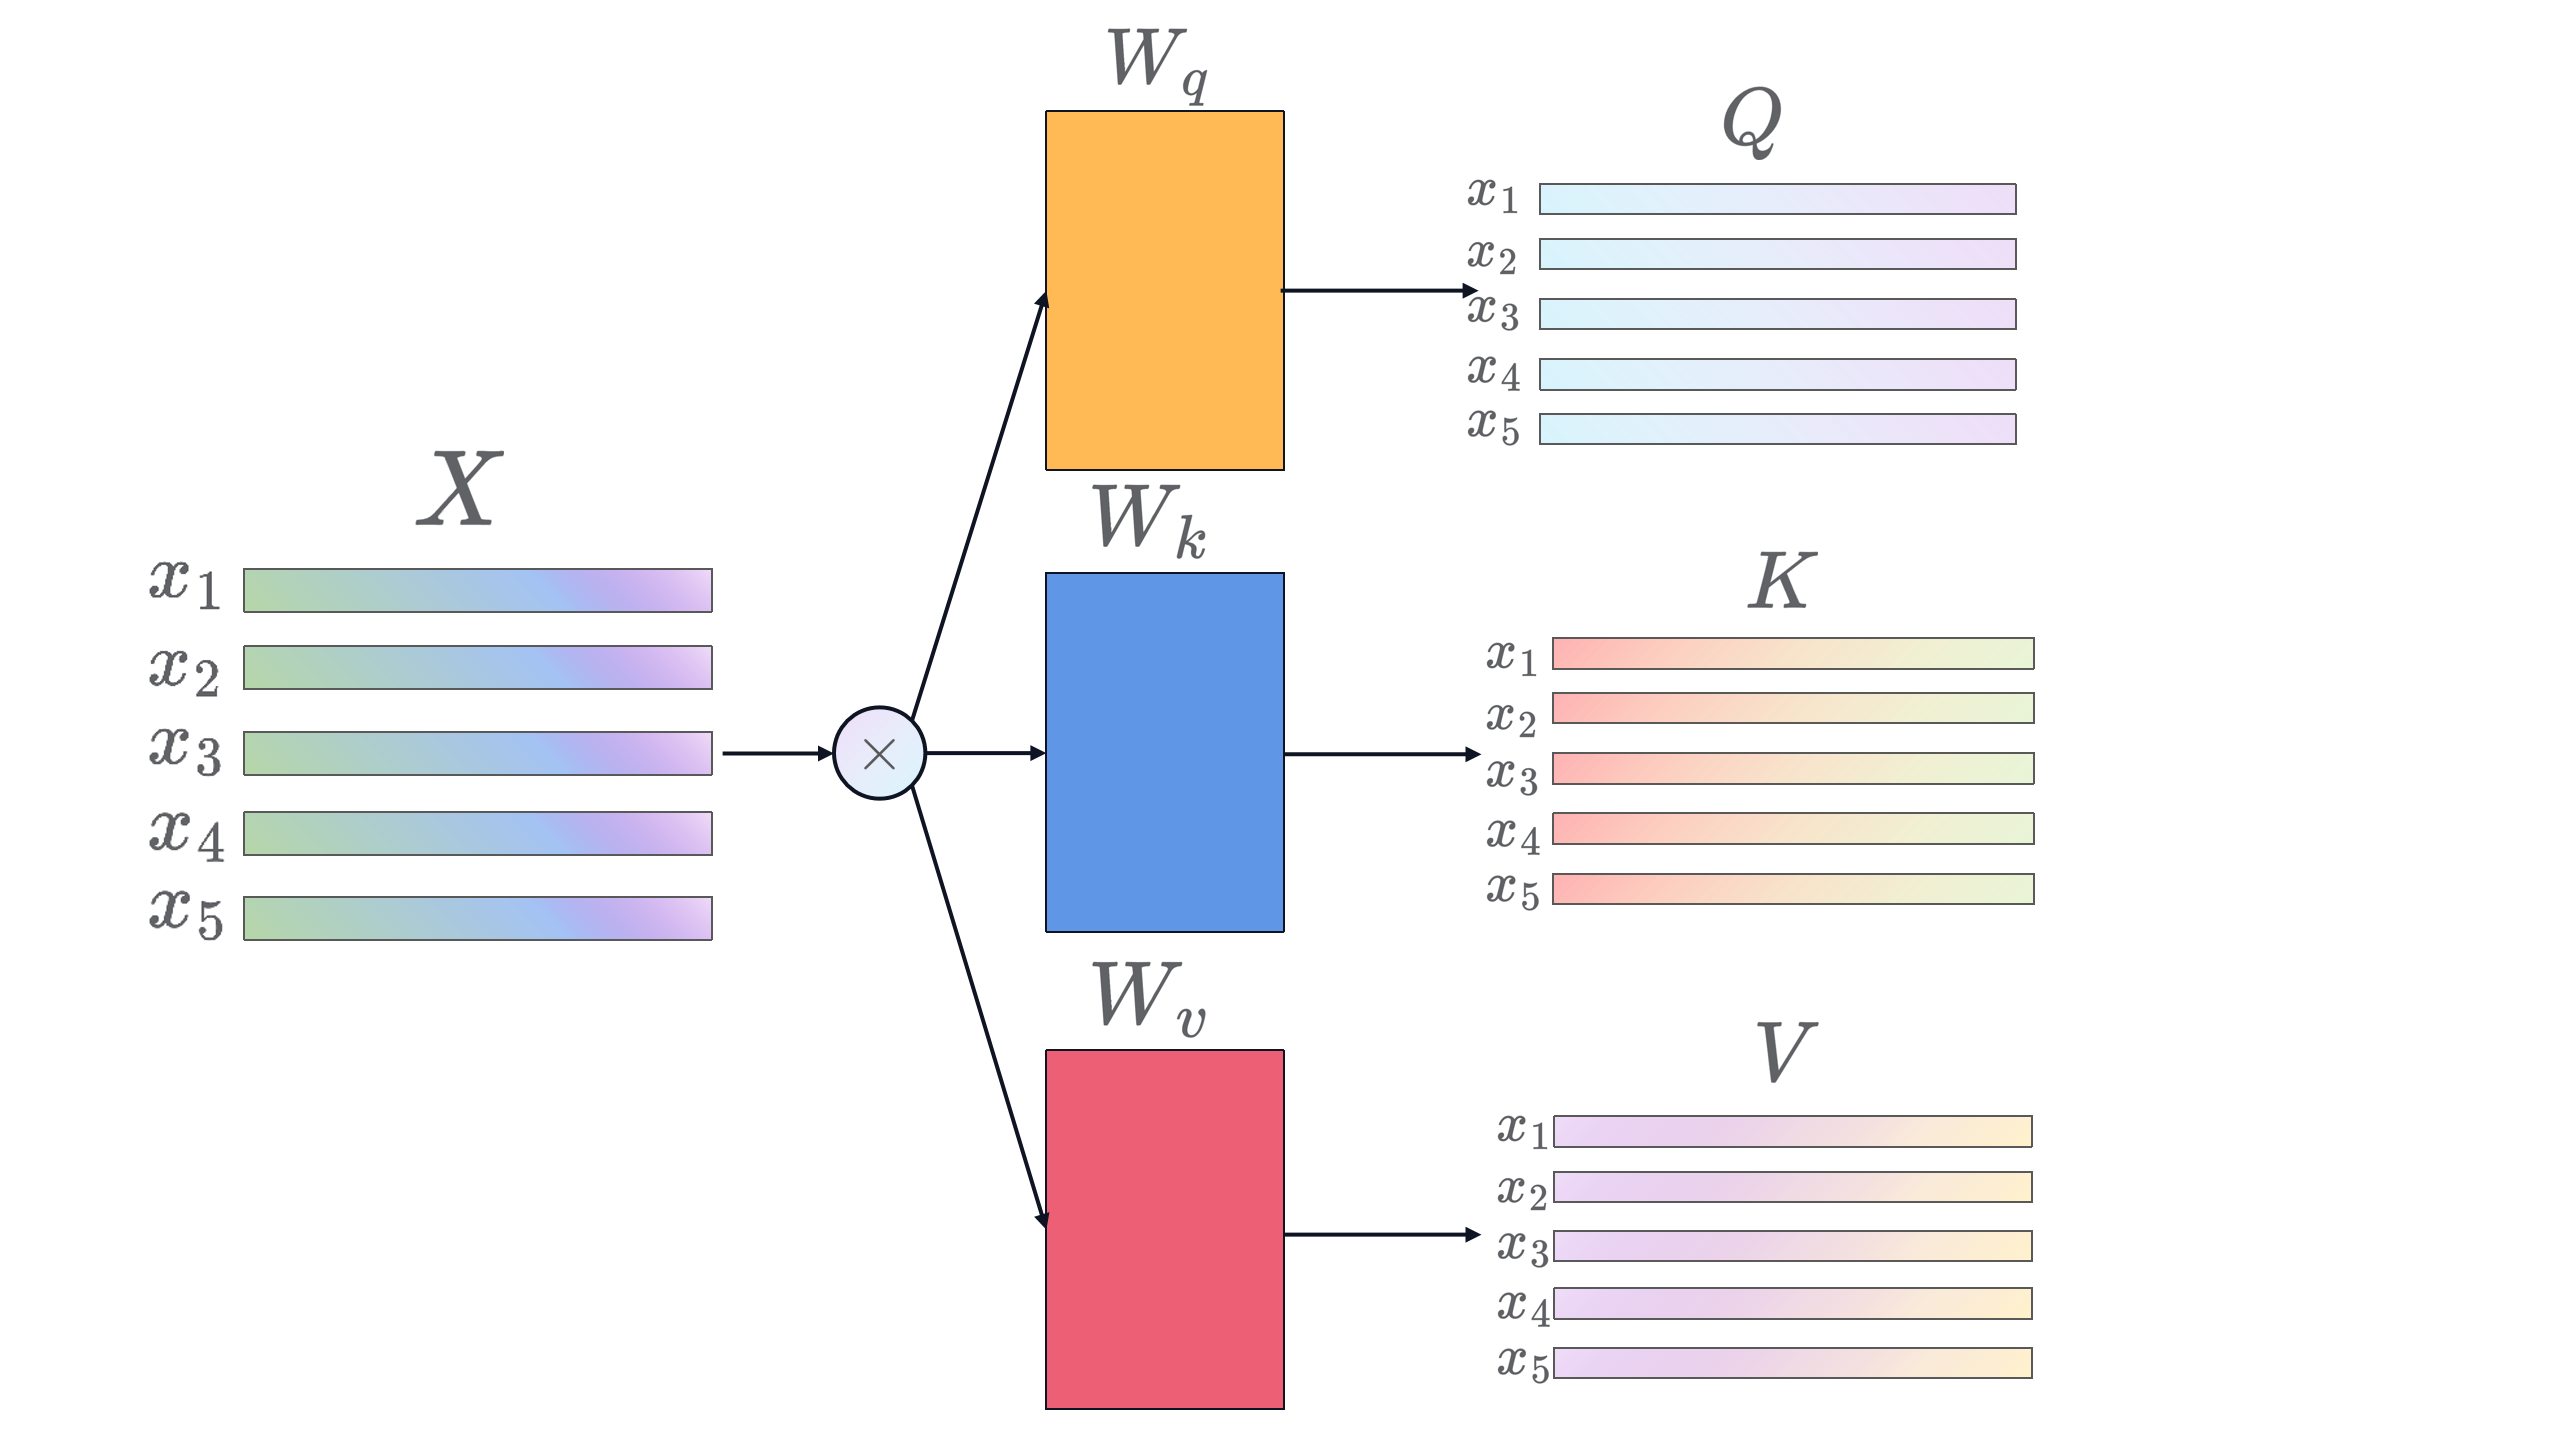
\includegraphics[width=0.75\columnwidth]{image/chap03/img308.png}
	\caption{将X经过三个线性变换后得到Q、K、V}
	\label{img308}
\end{figure}

\begin{figure}[h]
	\begin{minipage}[t]{0.5\linewidth}
		\centering
		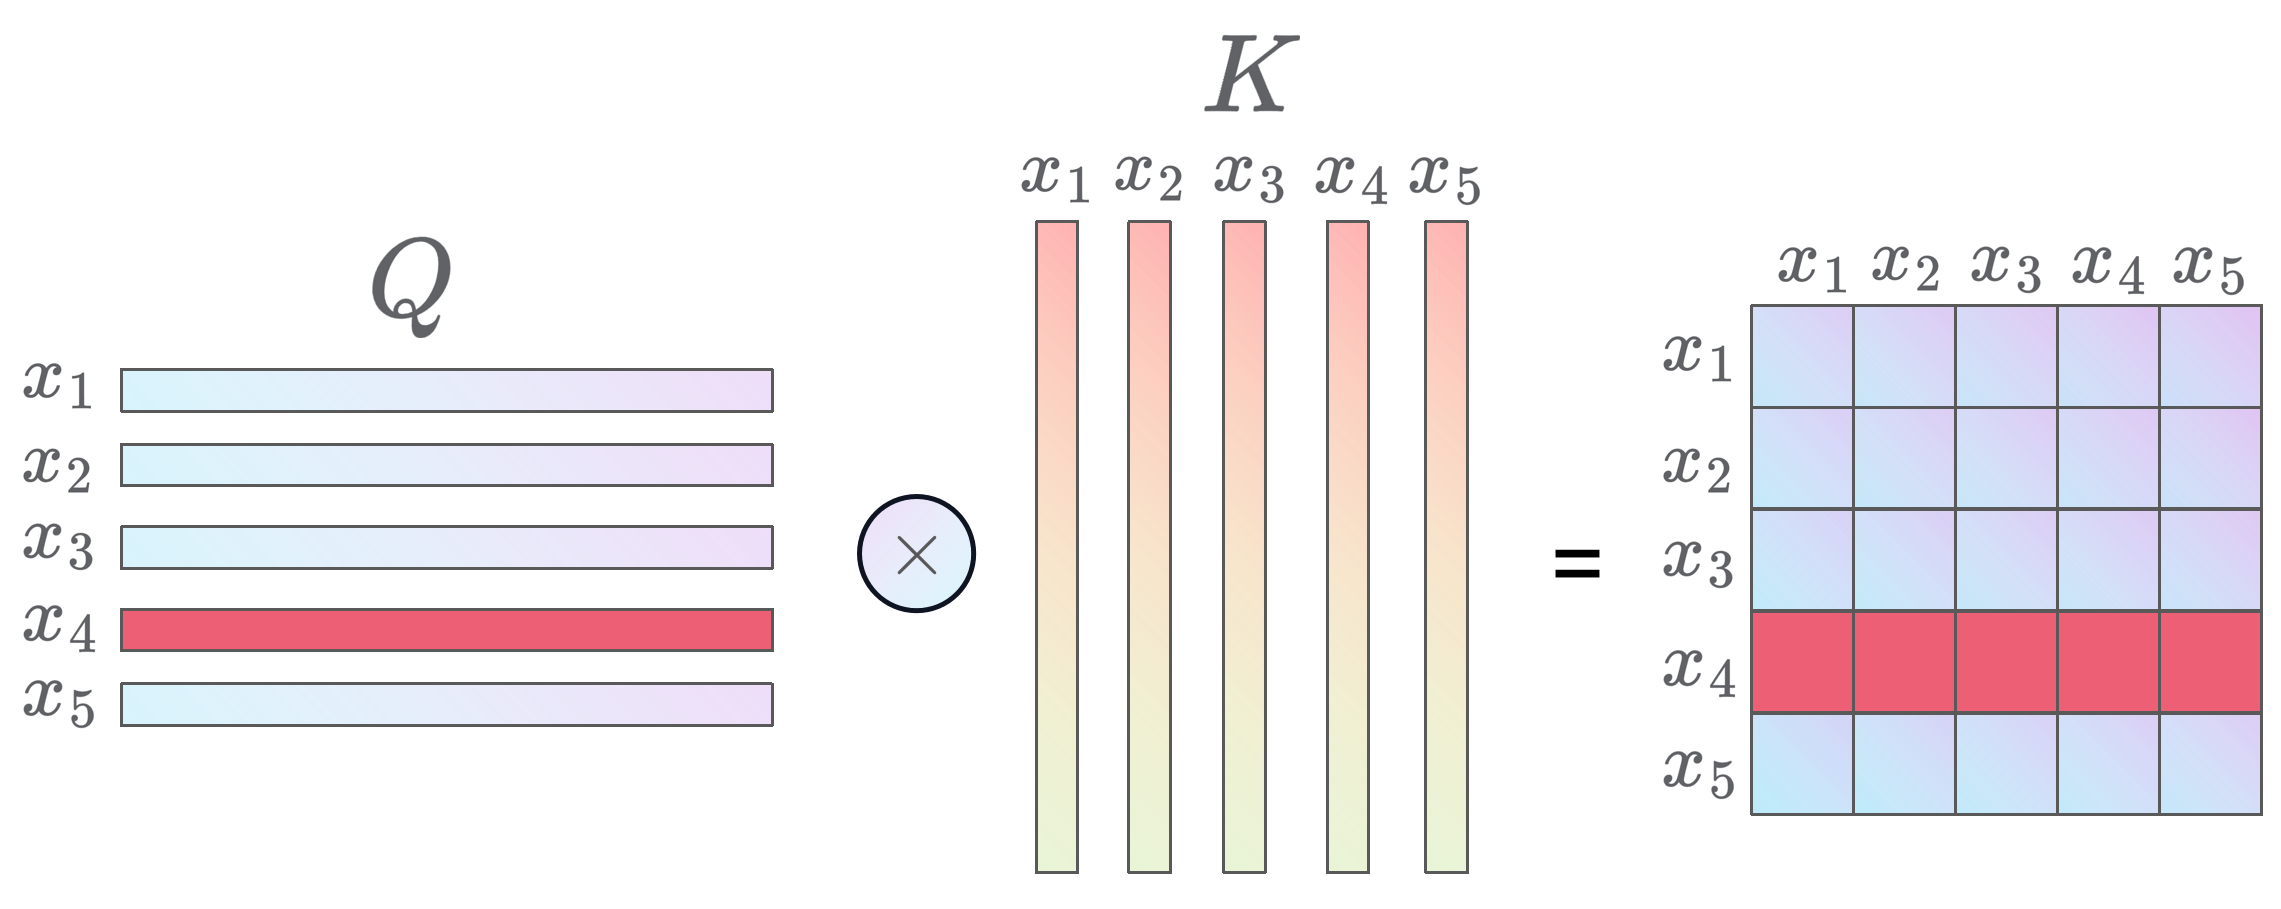
\includegraphics[scale=0.25]{image/chap03/img309.png}
		\caption{Q与K的转置相乘}
		\label{img309}
	\end{minipage}%
	\begin{minipage}[t]{0.5\linewidth}
		\centering
		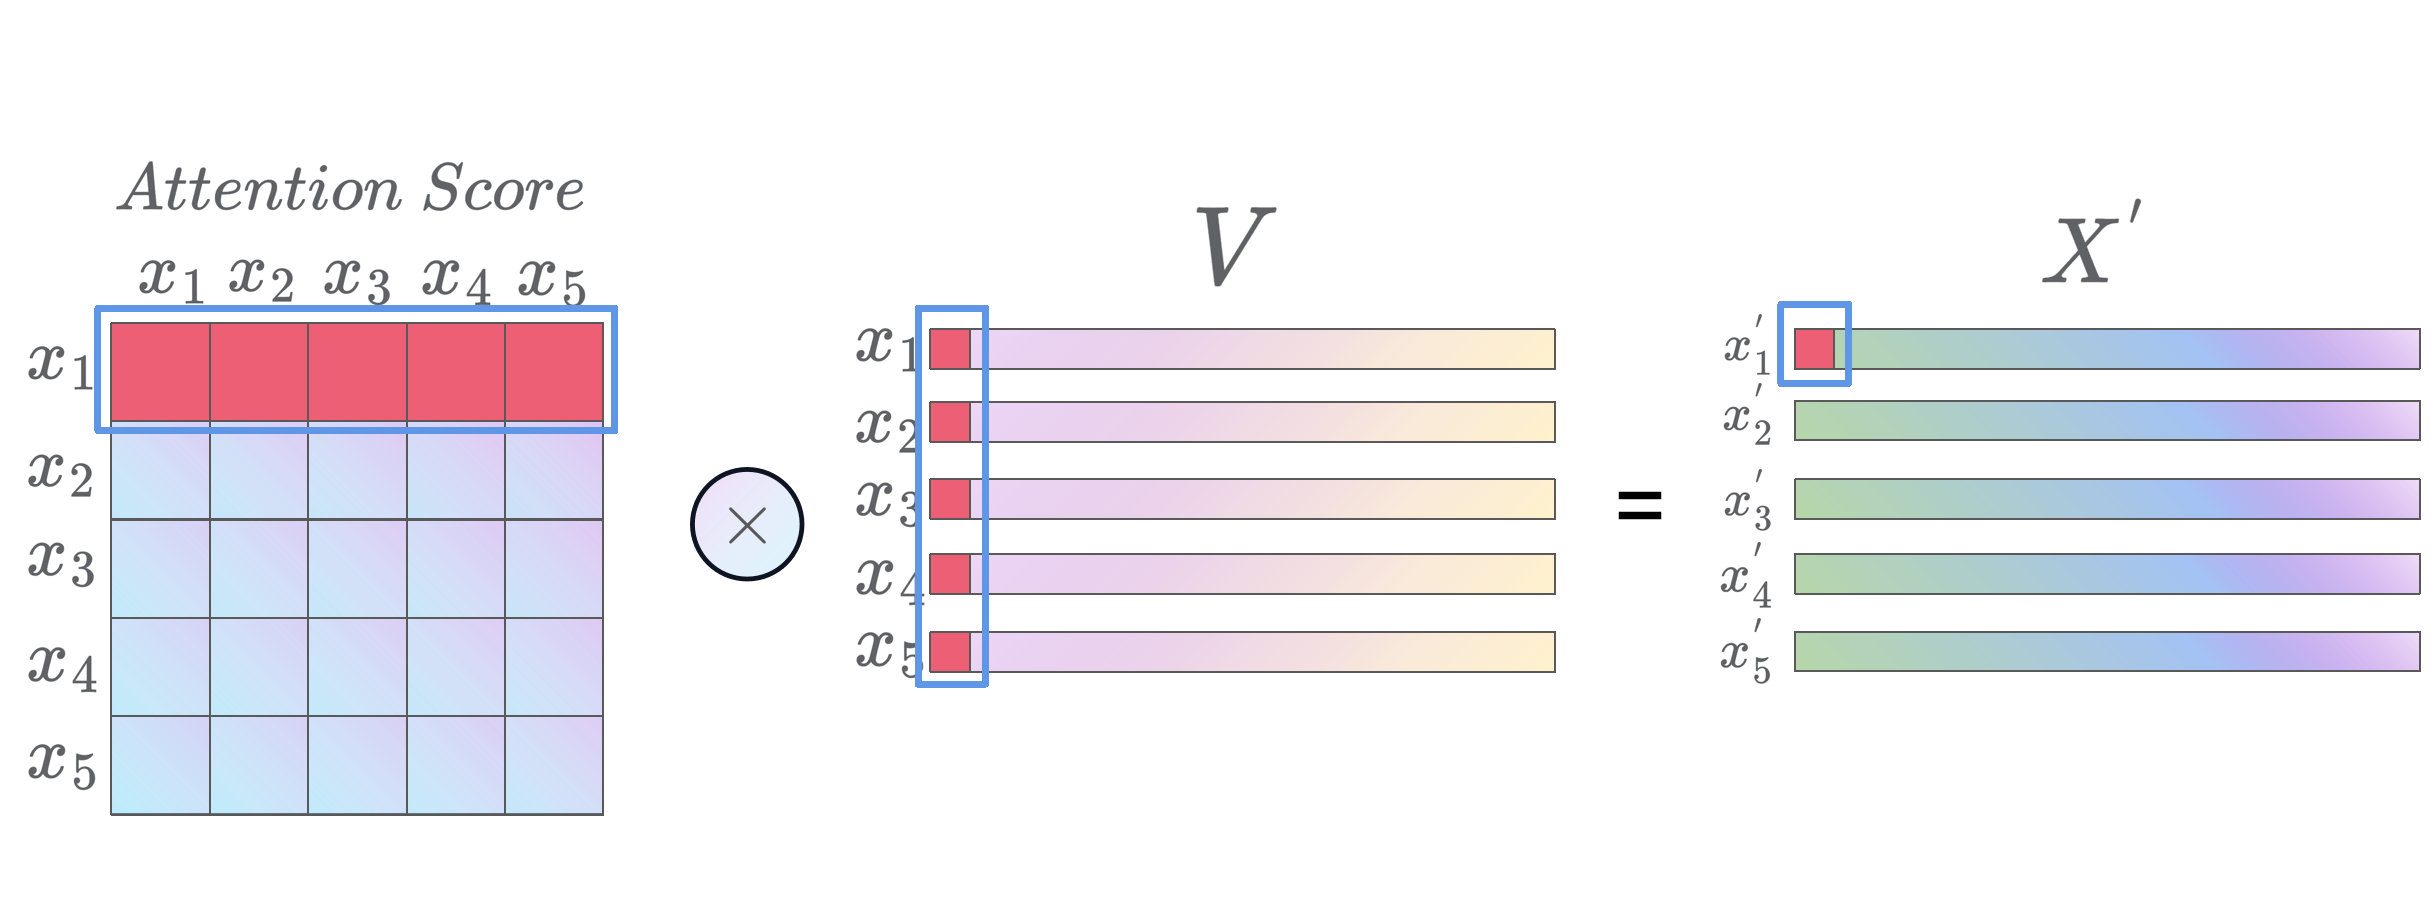
\includegraphics[scale=0.25]{image/chap03/img310.png}
		\caption{将得到的注意力权重矩阵与V相乘}
		\label{img310}
	\end{minipage}
\end{figure}

\subsubsection{将$Q$与$K$输入注意力打分函数得到注意力权重}
其中注意力打分函数的实现如下:

\begin{equation} \label{302}
	\begin{aligned}
		F(X)=softmax(\cfrac{QK^T}{\sqrt{D_k}})
	\end{aligned}
\end{equation}

注意力打分函数的运算由两部分组成:

\begin{itemize}
	\item [1)]
	第一部分是将$Q$与$K$的转置相乘,得到一个矩阵。该矩阵的第i行j列的元素为$x_i$与$x_j$的转置相乘得到的,代表“将$x_i$和$x_j$代入到注意力打分函数”这一操作。如图\ref{img309}所示,右边矩阵红色方块所在行为$Q$中代表$x_4$的行与$K$转置中代表$x_1,x_2,\cdots ,x_5$所在列相乘得到的。
	\item [2)]
	第二部分将所得矩阵各元素进行标准化,而后再进行一次softmax运算。这一步的作用是确保注意力打分函数得到的矩阵各元素都为位于[0,1]之间的权重。运算后得到的矩阵即为注意力权重(Attention Score)矩阵。
\end{itemize}

在图\ref{img303}的机器翻译任务中,第4行1列元素的值代表在翻译“深度”字时,“我”字所提供的信息权重。

\subsubsection{将得到的注意力权重矩阵与$V$相乘}
如图\ref{img310}所示,注意力权重矩阵第一行与$V$相乘得到的$X^{'}$中的第一行元素$x_1^{'}$,可以看作利用所给权重结合$x_1,\cdots ,x_5$信息后的$x_1$。因此最终运算得到的矩阵即代表按照所给权重结合全局信息后的元素$x_1^{'}, \cdots ,x_5^{'}$按行排列而成的矩阵$X^{'}$。

\subsubsection{最终对$X^{'}$再做一次线性变换使之恢复为原来的矩阵形状后输出}
这里所乘的线性变换矩阵$W_0$也为可学习的参数。

综上所述,总体的过程如图\ref{img311}所示。

\begin{figure}[h]
	\centering
	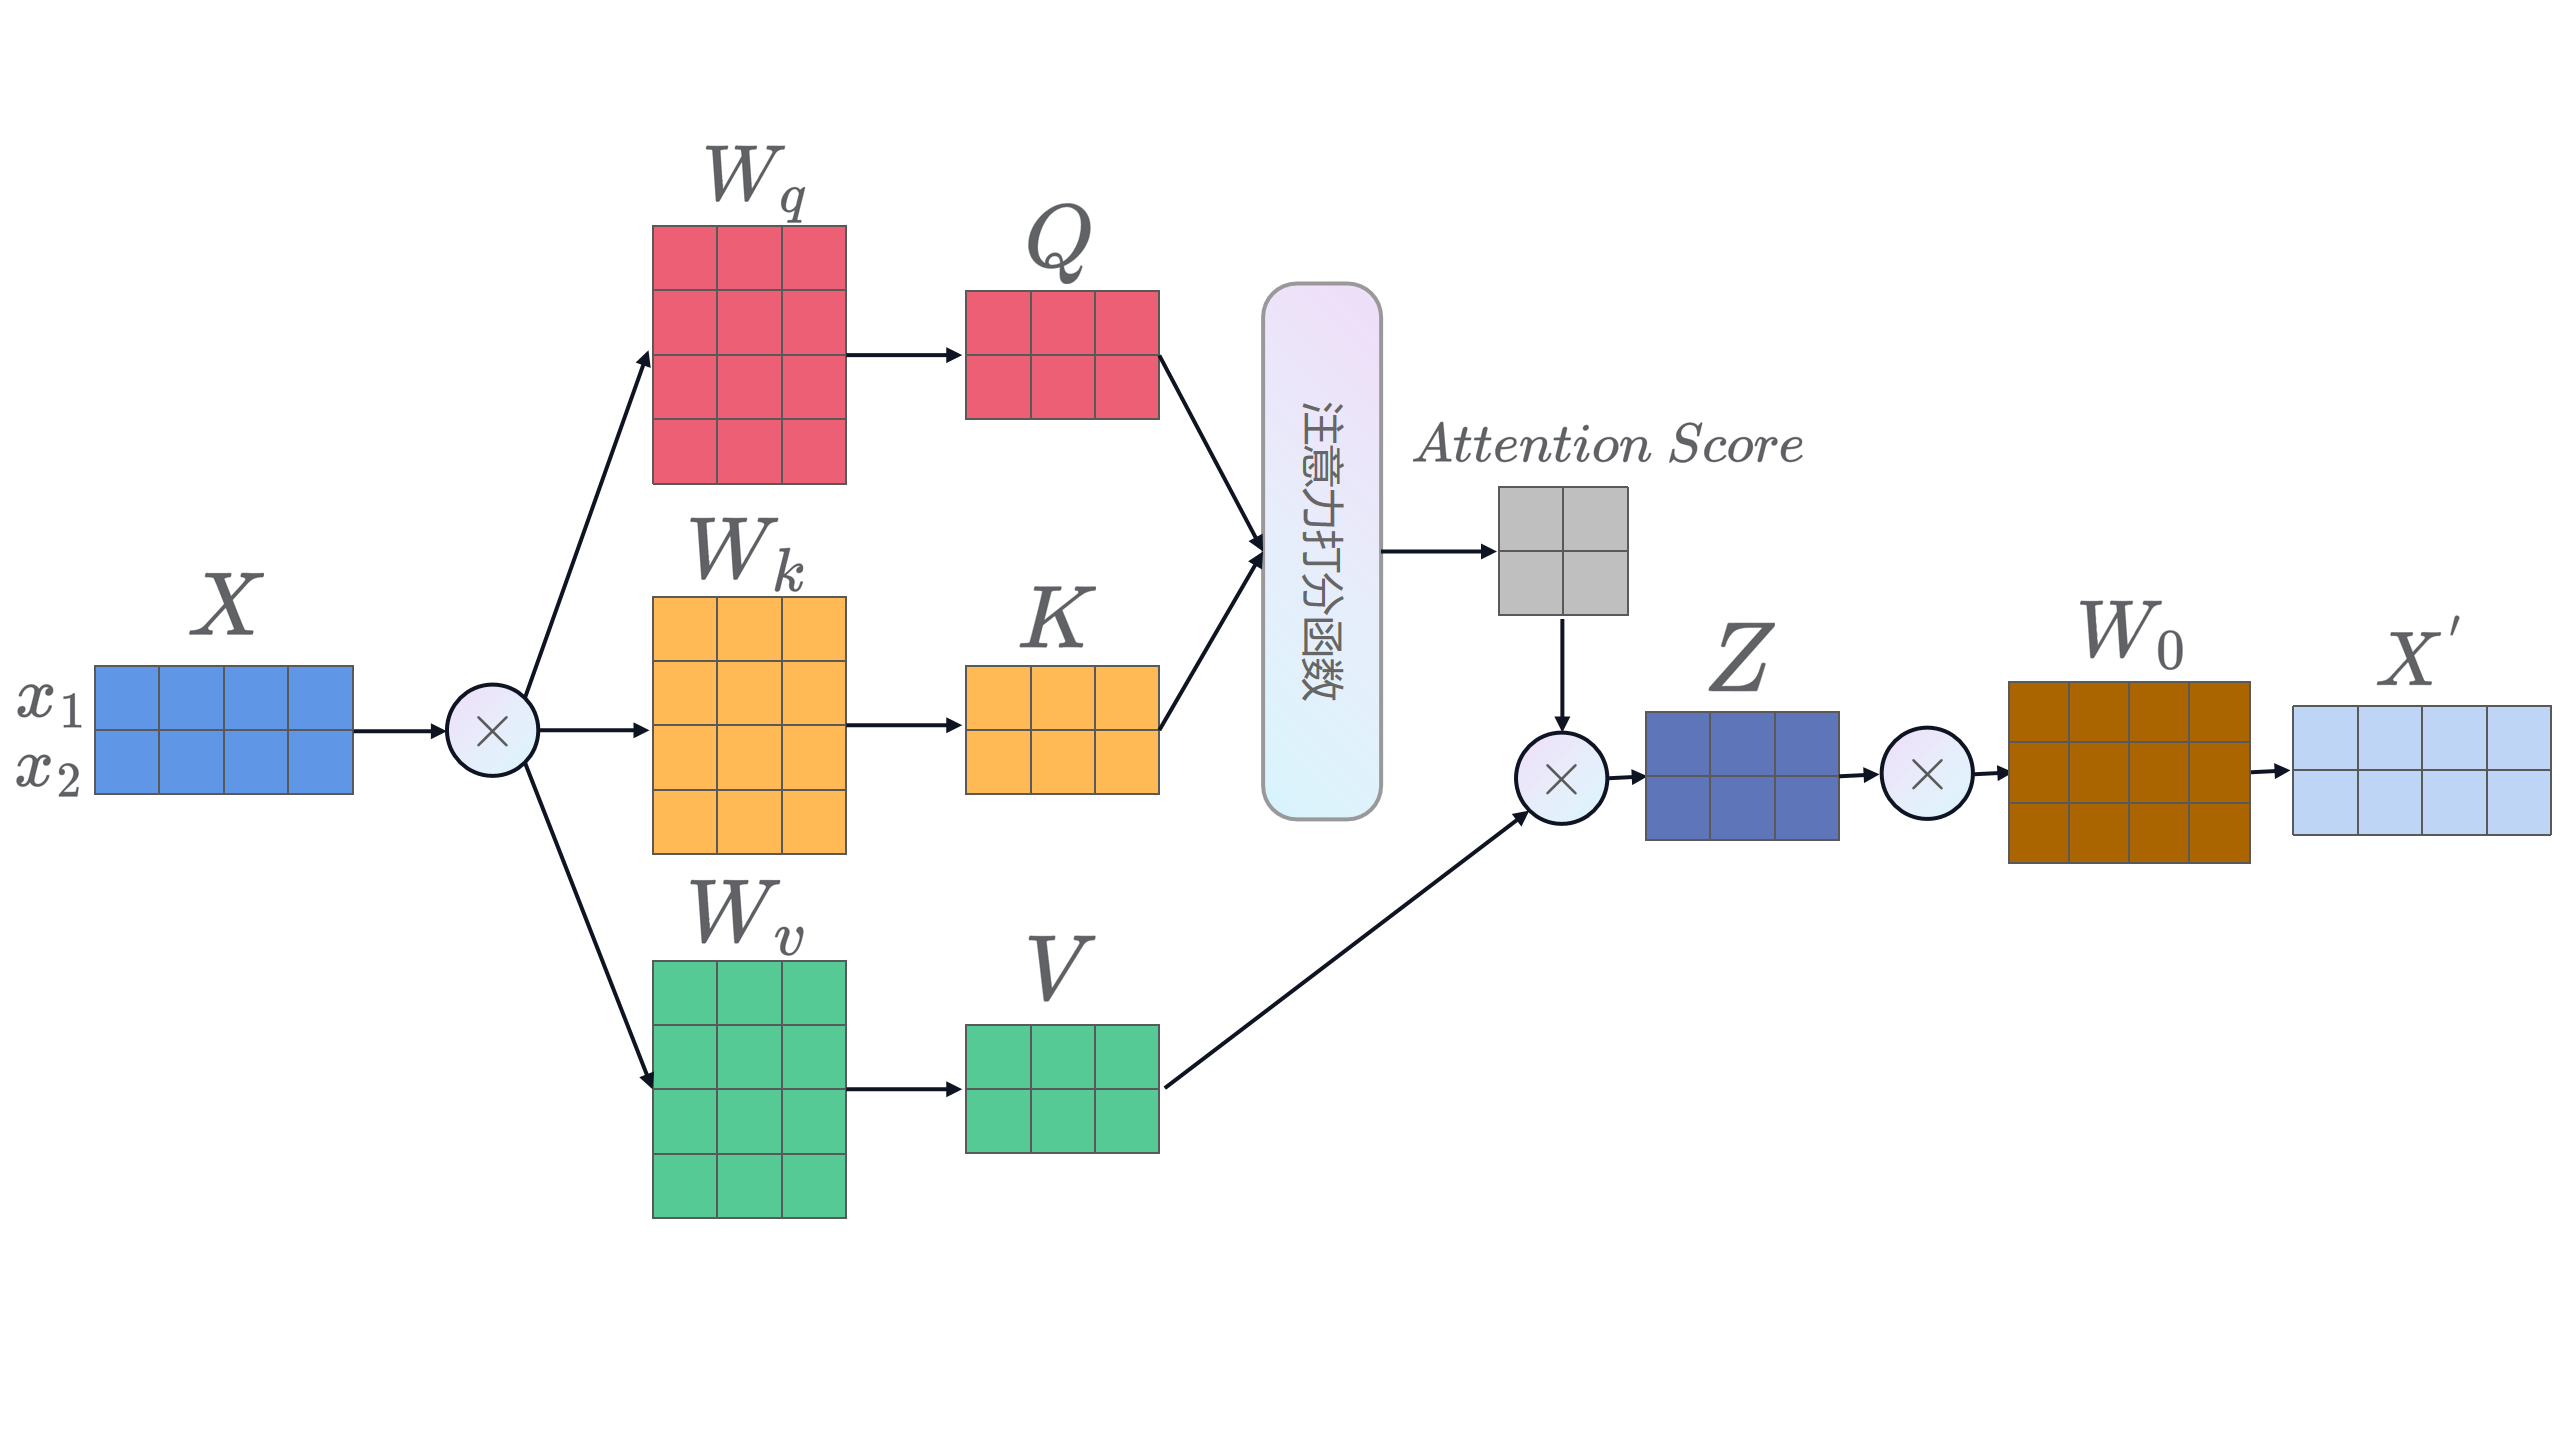
\includegraphics[width=0.75\columnwidth]{image/chap03/img311.png}
	\caption{自注意力机制的实现}
	\label{img311}
\end{figure}

\subsection{多头注意力机制}

\begin{figure}[h]
	\centering
	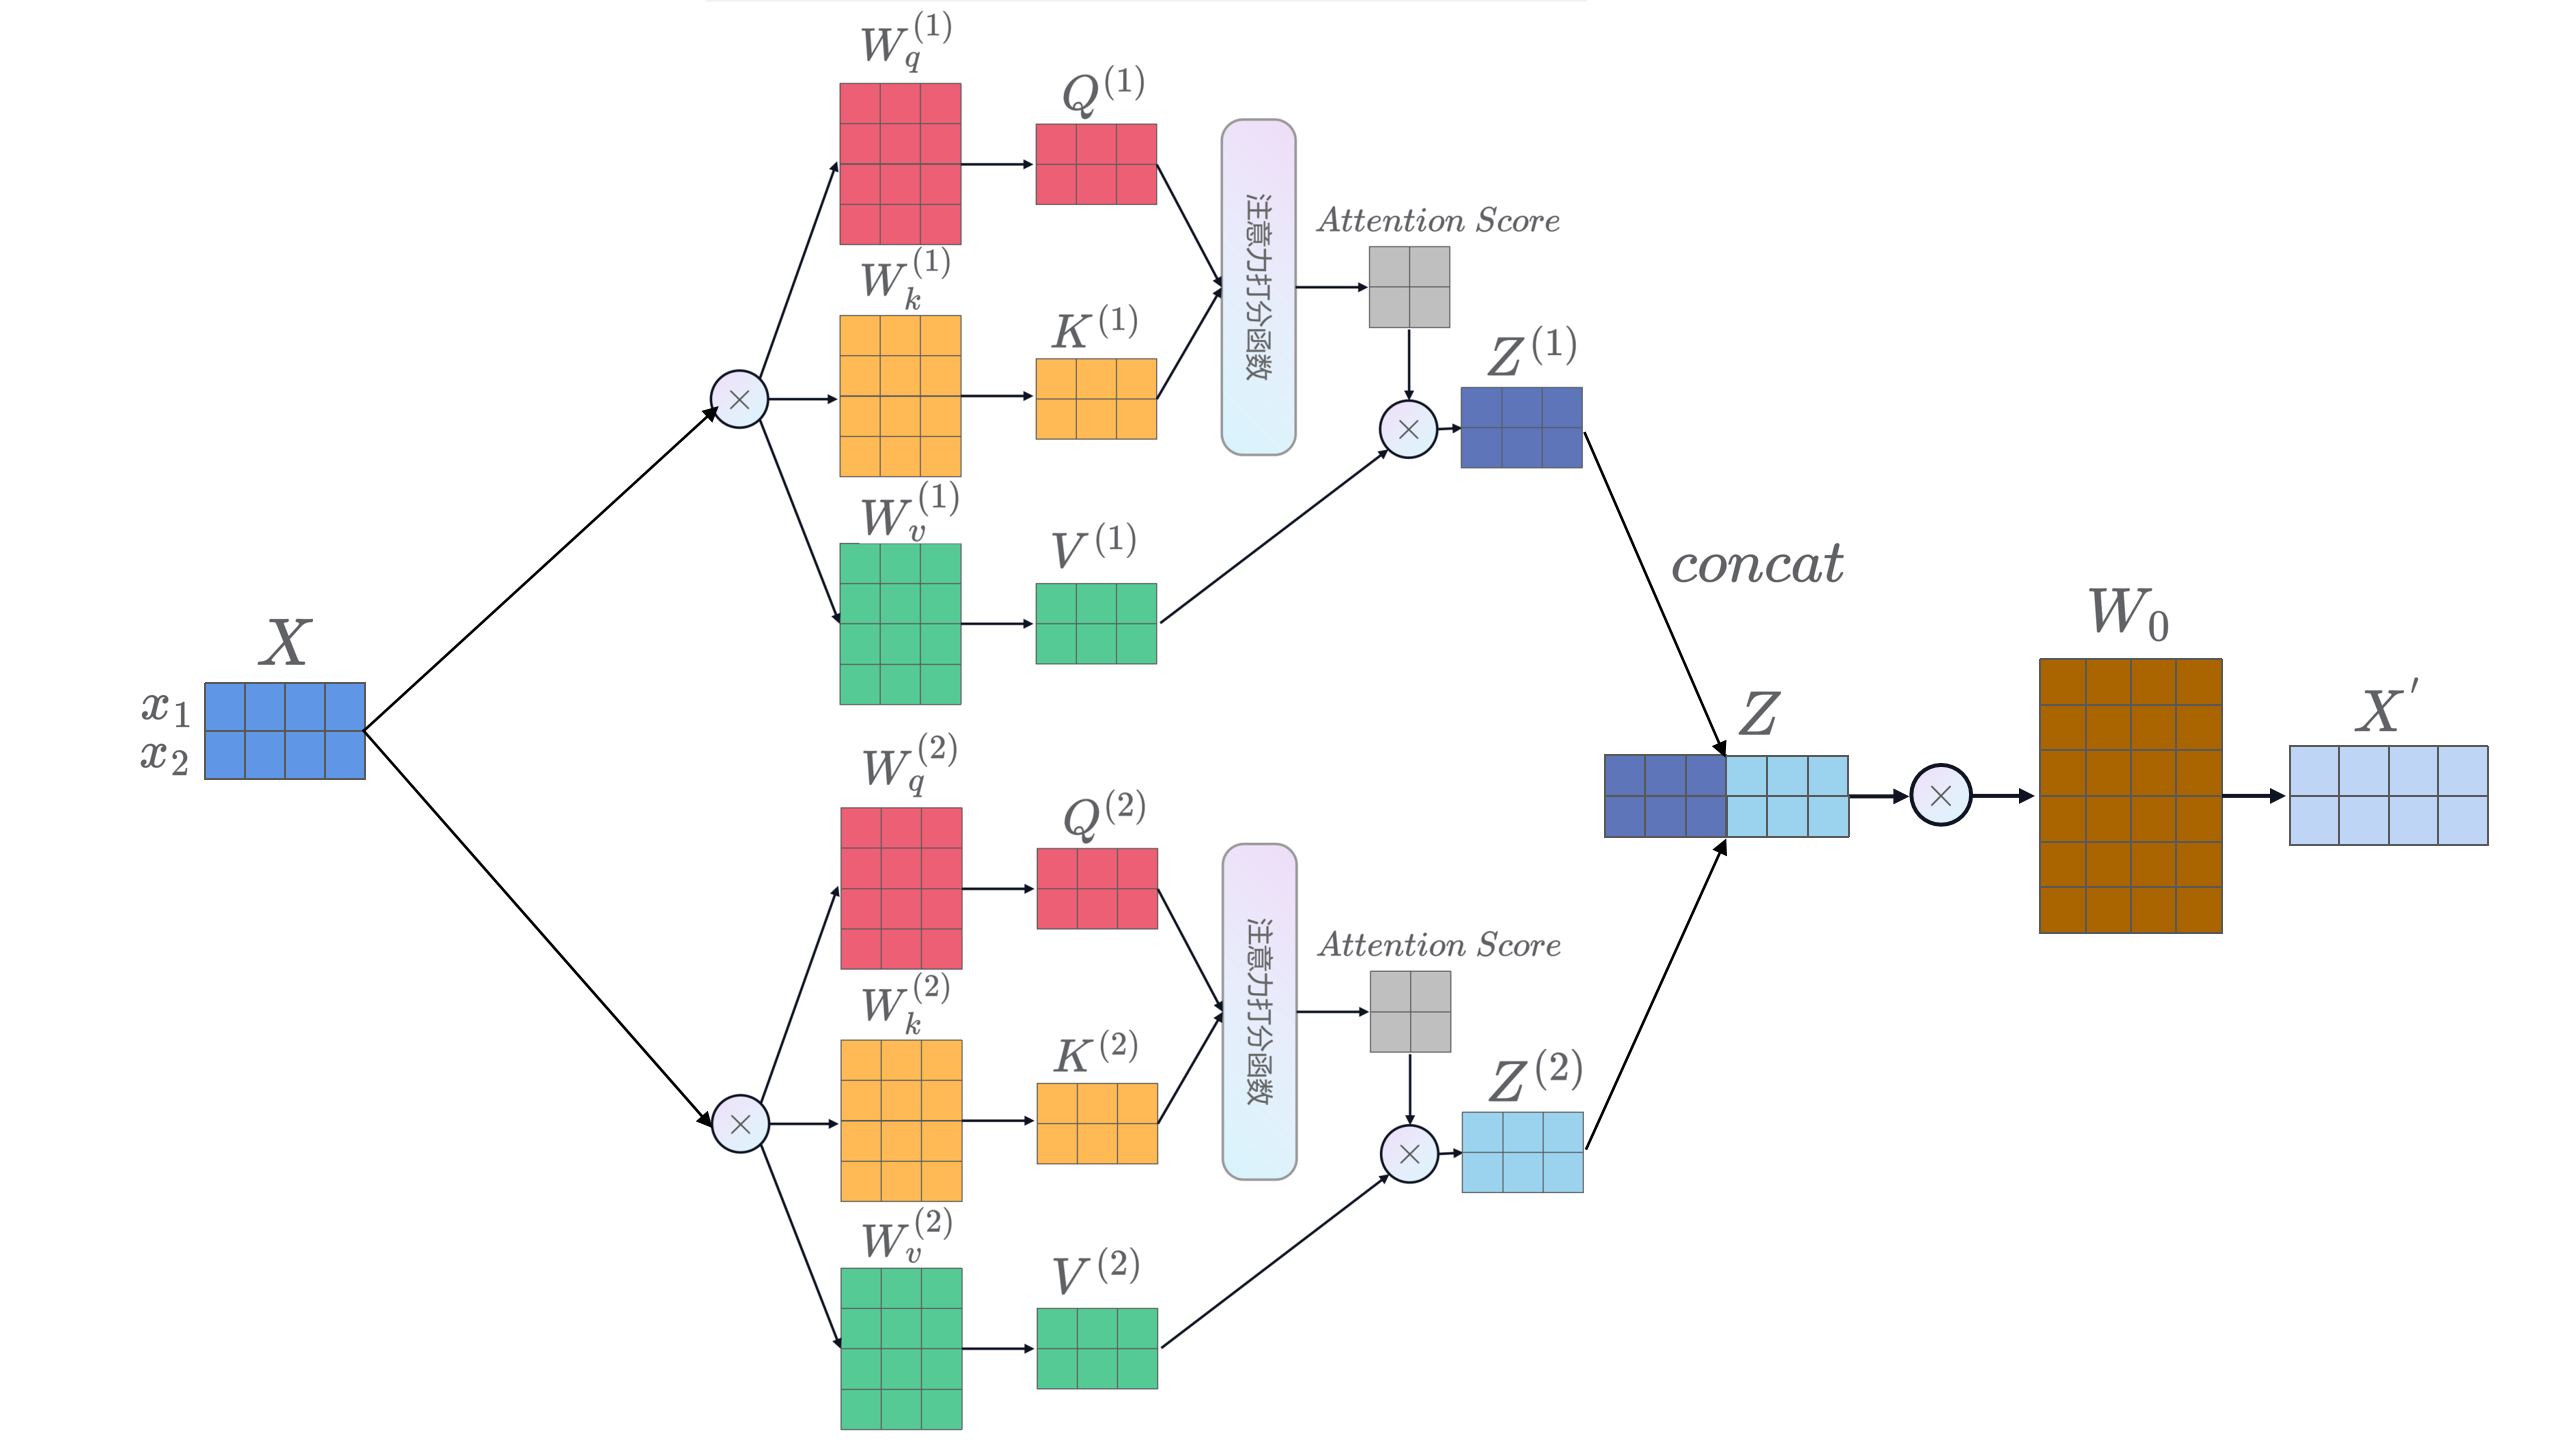
\includegraphics[width=0.9\columnwidth]{image/chap03/img312.png}
	\caption{二头注意力机制的实现}
	\label{img312}
\end{figure}

正如CNN中不同的卷积核能学习到不同的特征,研究人员相信通过增加注意力机制中的注意力打分函数个数,可以让模型学习到不同的信息权重特征,进而优化模型表现。

比如图\ref{img312}所示的二头注意力机制,通过两组线性变化$(W_q^{(1)},W_k^{(1)},W_v^{(1)})$和$(W_q^{(2)},W_k^{(2)},W_v^{(2)})$将$X$映射成两组$Q,K,V$后,通过自注意力机制得到$z^{(1)},z^{(2)}$;将得到的$z^{(1)},z^{(2)}$经过concat连接后,再对其进行一次线性变换,恢复原形状后输出。

其余多头注意力机制的实现与二头注意力机制的实现是相似的,区别仅在于n头注意力机制的注意力打分函数个数为n个。

\section{Transformer在CV领域的应用与改进}
将自注意力机制运用于CV领域是现今Transformer发展的一个重要方向。一张图片由一个个像素点组成,如果直接将Transformer应用在图片上就需要每个像素点跟其他所有像素点都算一下权重。那么一张分辨率为$n*m$的图片就要计算$(n*m)*(n*m$)次注意力机制。随着图片像素的增加,运算的复杂度就会呈现平方级增长。

为了应对这个问题,提出了不同的Transformer模型的改进方法。下面介绍几种典型的改进方法:

\subsection{与卷积相结合的CV Transformer}
在这类模型中,先利用卷积层将图像进行降采样后,使其分辨率降低。然后再将其输入到Transformer中。

\subsection{Axial-Attention(轴向注意力)}
 Axial-Attention对一个像素进行自注意力机制的计算时,不是让它与其他所有像素做注意力机制,而是先只与同行像素做注意力机制后,再与同列像素做注意力机制。在这种改进方法下,单个像素的运算量从原来的$o(n*m)$变成了现在的$o(m+n)$,使得计算量大大降低。
 
 由于第一步的轴向注意力操作能使每个像素点就蕴含了整行的信息,而第二步的轴向注意力操作能使得这些已经蕴含了整行信息的像素点之间进行同列信息的相互结合,于是研究人员认为这种串联的处理方法不仅使得单个像素点能结合所在行与列的信息,而且还能让单个像素点结合整个图象的全局信息。
 
 轴向注意力机制的具体操作如图\ref{img313}。
 \begin{figure}[h]
 	\centering
 	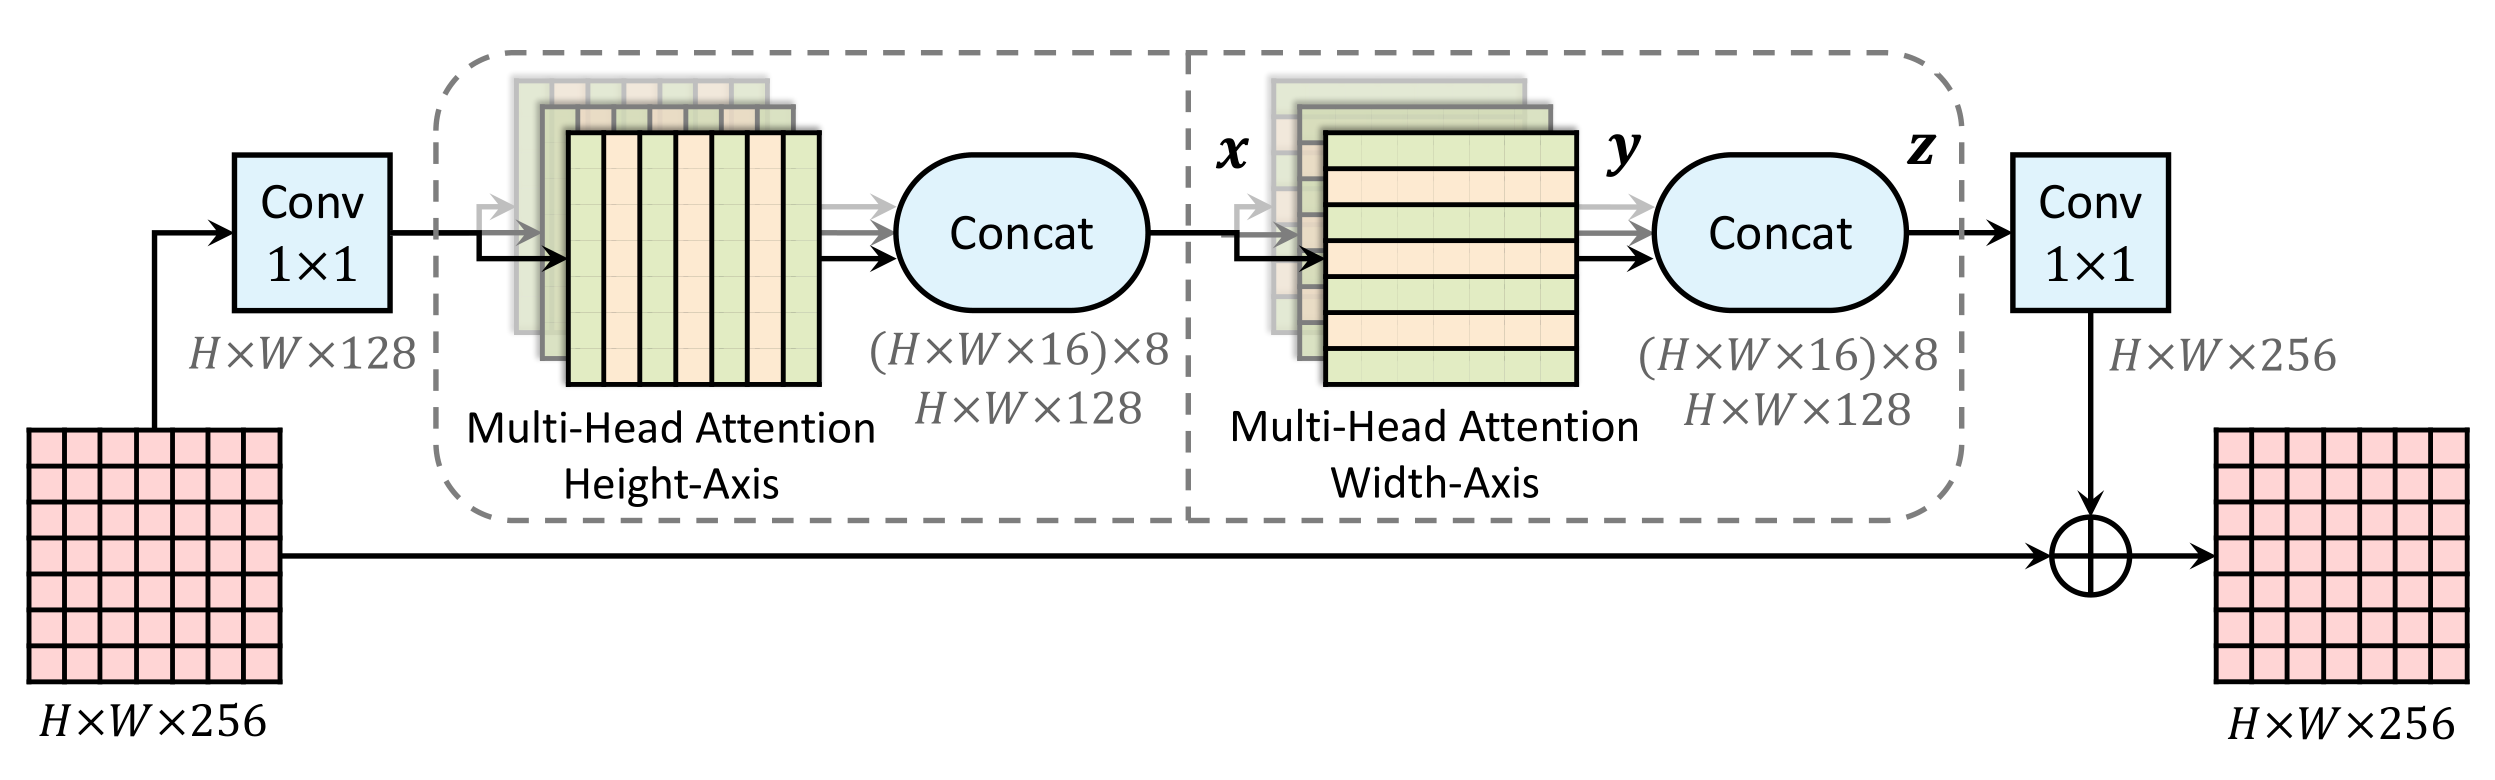
\includegraphics[width=0.75\columnwidth]{image/chap03/img313.png}
 	\caption{Axial-Attention模型的结构\cite{wang2020axial}}
 	\label{img313}
 \end{figure}

\subsection{ViT神经网络对注意力机制的实现}
 ViT神经网络对传统注意力机制的改进方法是把先将图像进行分割,分割成一个个固定大小的patch,将这个patch看成一个大像素(每个patch展平当作一个向量),然后在让所有这些“大像素”向量之间做自注意力机制。这时就等价于对一张更低像素图片做注意力机制,达到将计算量变少的目的。具体ViT神经网络的实现如图\ref{img314}所示。
 
 \begin{figure}[h]
 	\centering
 	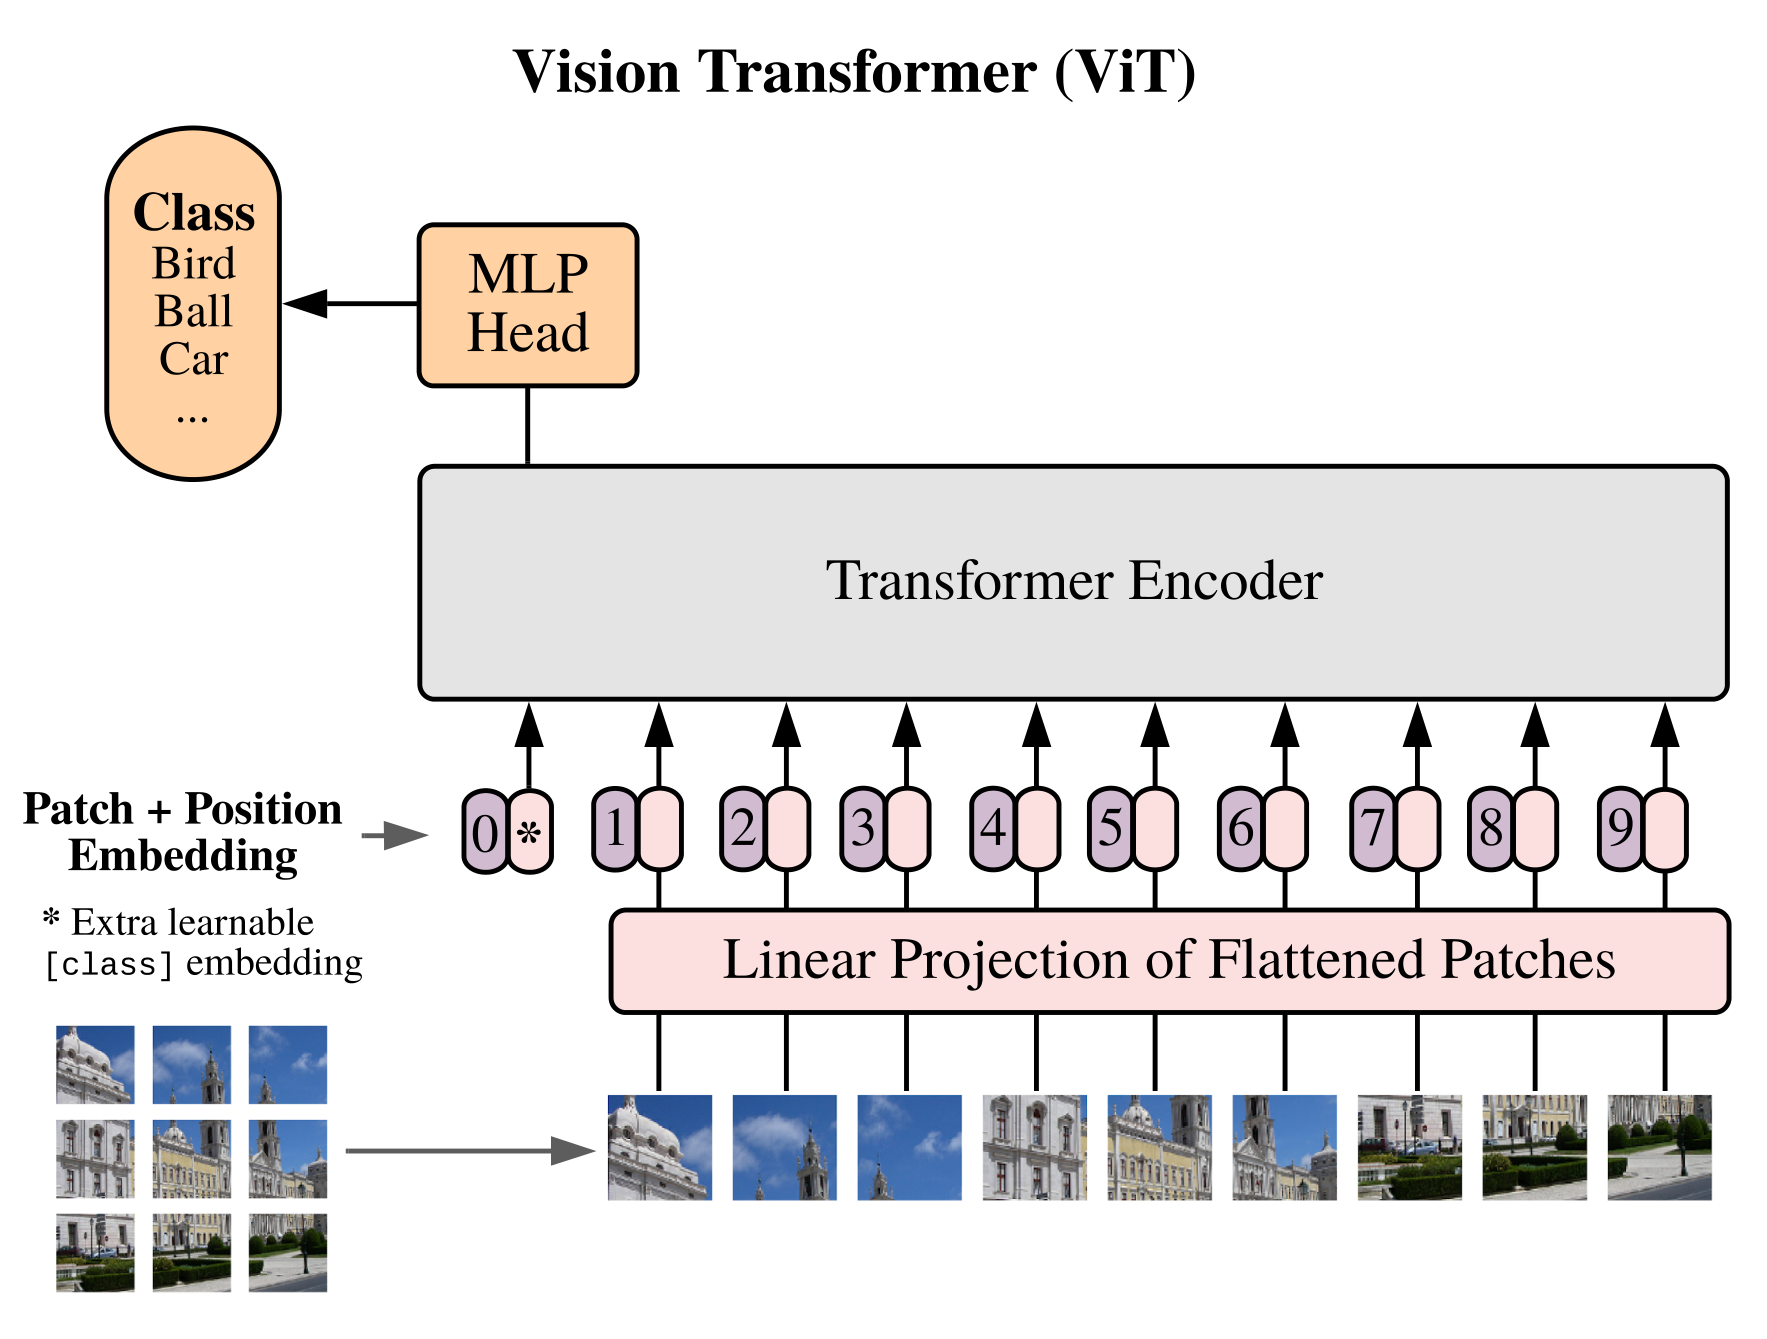
\includegraphics[width=0.5\columnwidth]{image/chap03/img314.png}
 	\caption{ViT模型的结构\cite{dosovitskiy2020image}}
 	\label{img314}
 \end{figure}

\hspace*{\fill} \

\hspace*{\fill} \

\hspace*{\fill} \

\hspace*{\fill} \

\subsection{Swin Transformer}
与ViT的改进不同,Swin Transformer在将图像进行分割成patch后,并不是在这些patch间运算注意力机制,而是对patch内的各像素间做注意力机制。这部分操作是在W-MSA内完成的(即W-MSA(Window Attention):分成一个个patch,然后在patch内部做自注意力机制,做完后再拼接到一起)。虽然这样运算能因像素点减少而使得运算量降低,但由于patch与patch是相互独立,缺乏联系的,而导致单个像素无法很好地融合整个图像的信息。

于是Swin Transformer在W-MSA完成后又引入了SW-MSA操作,即采用滑动窗口后的再分割来规避上述缺陷。具体操作见图\ref{img315}。

 \begin{figure}[h]
	\centering
	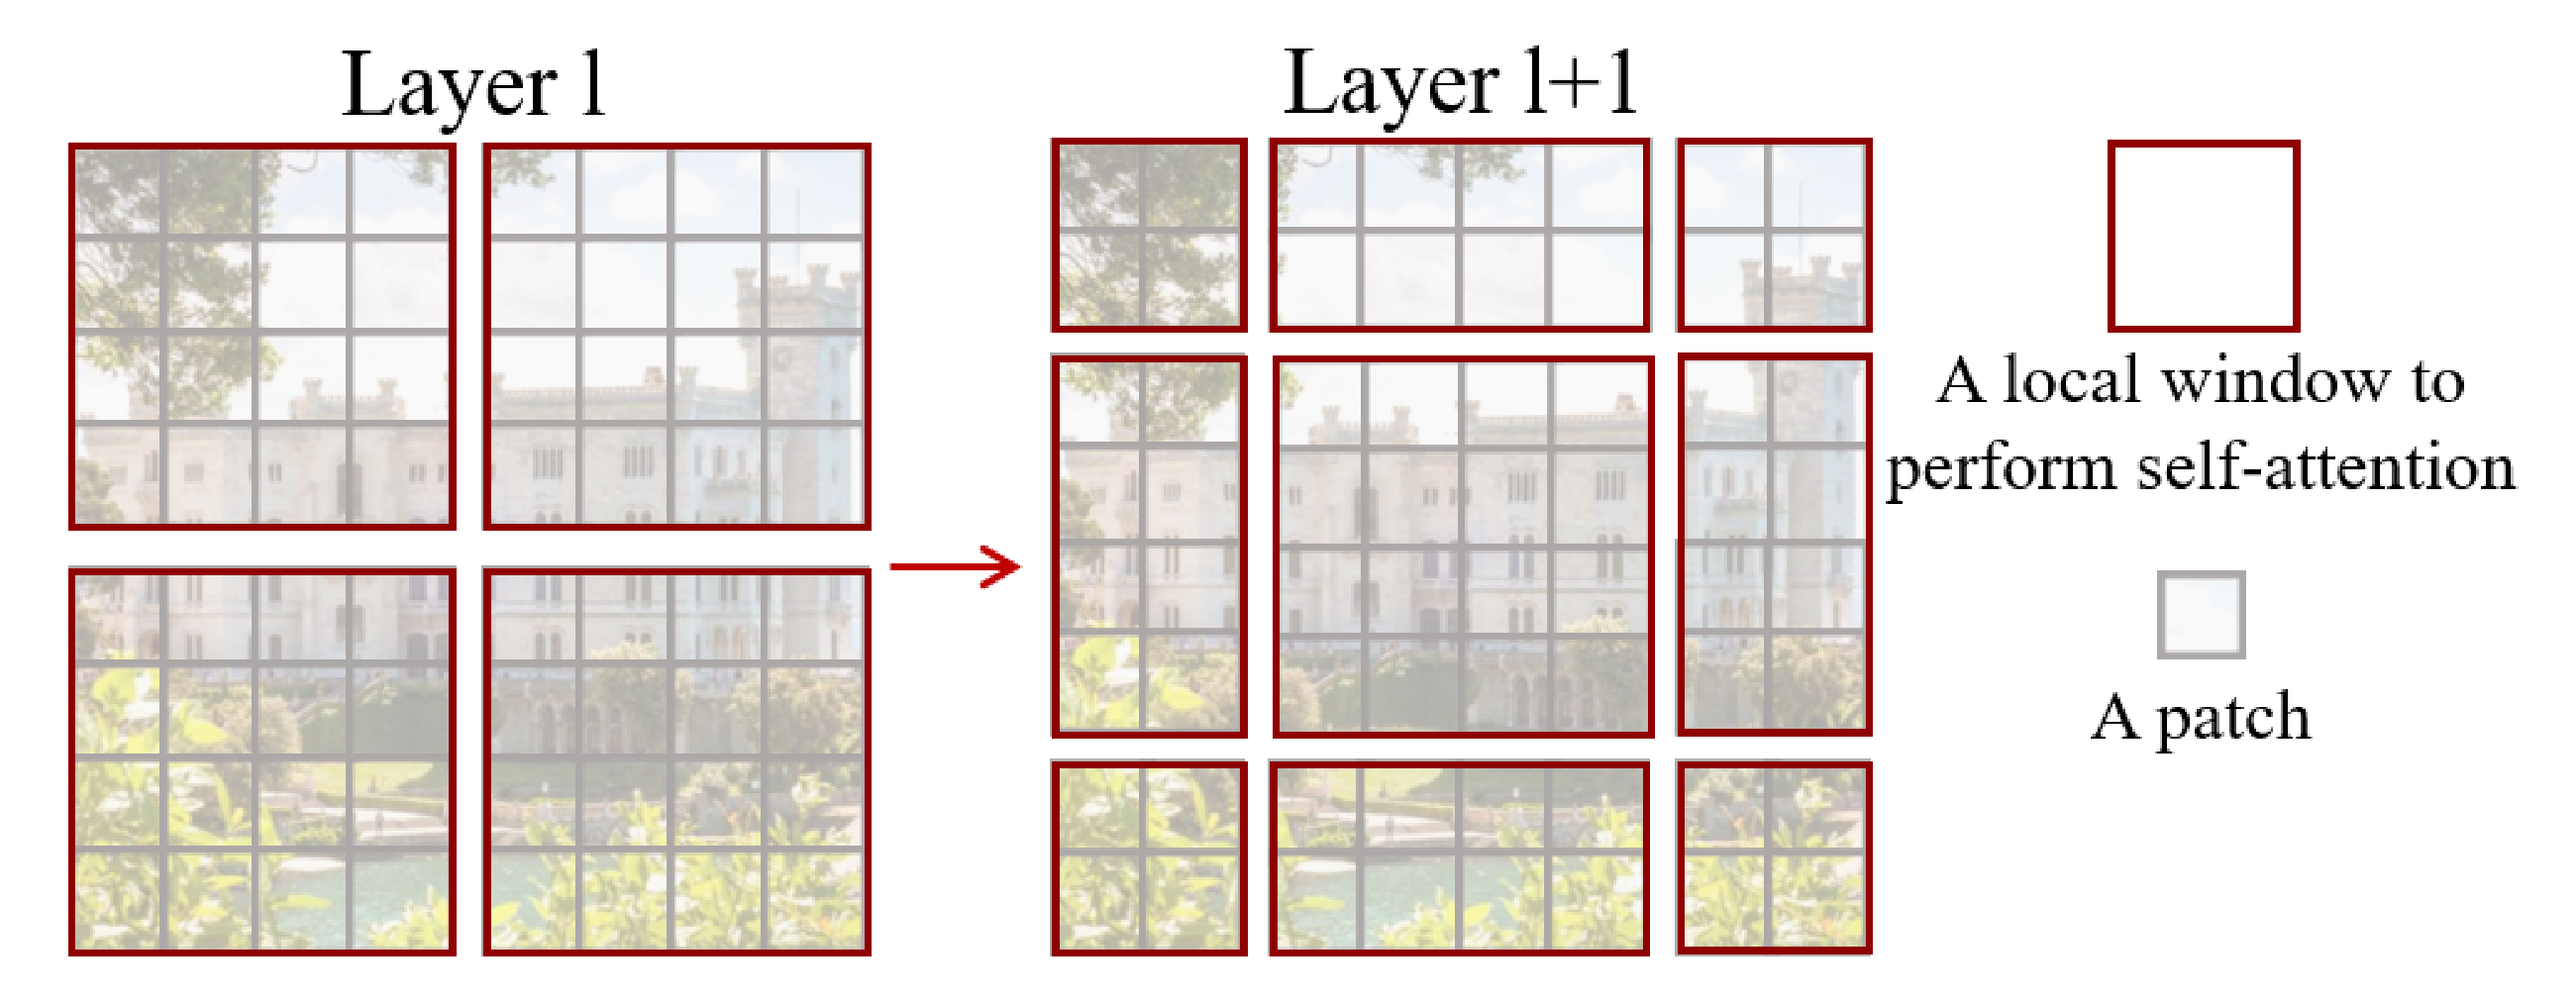
\includegraphics[width=0.75\columnwidth]{image/chap03/img315.png}
	\caption{Swin Transformer中的SW-MSA操作\cite{liu2021swin}}
	\label{img315}
\end{figure}
 
 如图\ref{img315}所示,整个过程是首先由W-MSA做上图左边四个patch的自注意力;然后采用滑动窗口的再分割得到上图右边的9个patch,再在这九个patch内部进行自注意力的运算。此时经过SW-MSA的操作后就使得单个像素能更好的融合整个图像的信息。
 
 \section{SwinTransformer的优势}
 在上述四种改进方法中,Swin Transformer模型在图像分类、目标检测、图像分割等常见的CV领域都有更好的实现效果。经过分析,Swin Transformer模型相较于其他现有模型的优势可能存在如下几点:
 
 \begin{itemize}
 	\item [1)]
 	Swin Transfomer的W-MSA和SW-MSA设计使其计算复杂度为输入图像大小的线性计算复杂度,相较于其他模型显著降低。
 	\item [2)]
 	Swin Transfomer的Patch Merging层设计使得输入图像的分辨率随着层数的加深而不断减小,进而进一步降低整个模型的计算复杂度,使得更深层数神经网路模型的实现成为可能。而深层模型相较于浅层模型往往具有更好的效果。
 	\item [3)]
 	从每个patch的感知范围的角度,Swin Transformer中的层次化构建方式类似于CNN,在逐层缩小图片分辨率的同时,使得每个patch的感知范围扩大。而ViT等改进方法中每个patch的感知范围是固定的。
 \end{itemize}

由于Swin Transformer模型在CV领域具有良好的表现,本项目采用Swin Transformer模型的改进思路来实现将低精度光声重建图像优化为高精度光声重建图像的模型。
\newclearpage
\chapter{训练数据的生成与预处理}
\label{cha:usage-example}

\section{数据集的介绍}
本次项目采用的数据集为Skin Cancer MNIST: HAM10000。该数据集由10000张来自不同人群的皮肤镜图像组成。

数据集中的几张皮肤癌图片举例如图\ref{img401}。

\begin{figure}[h]
	\centering
	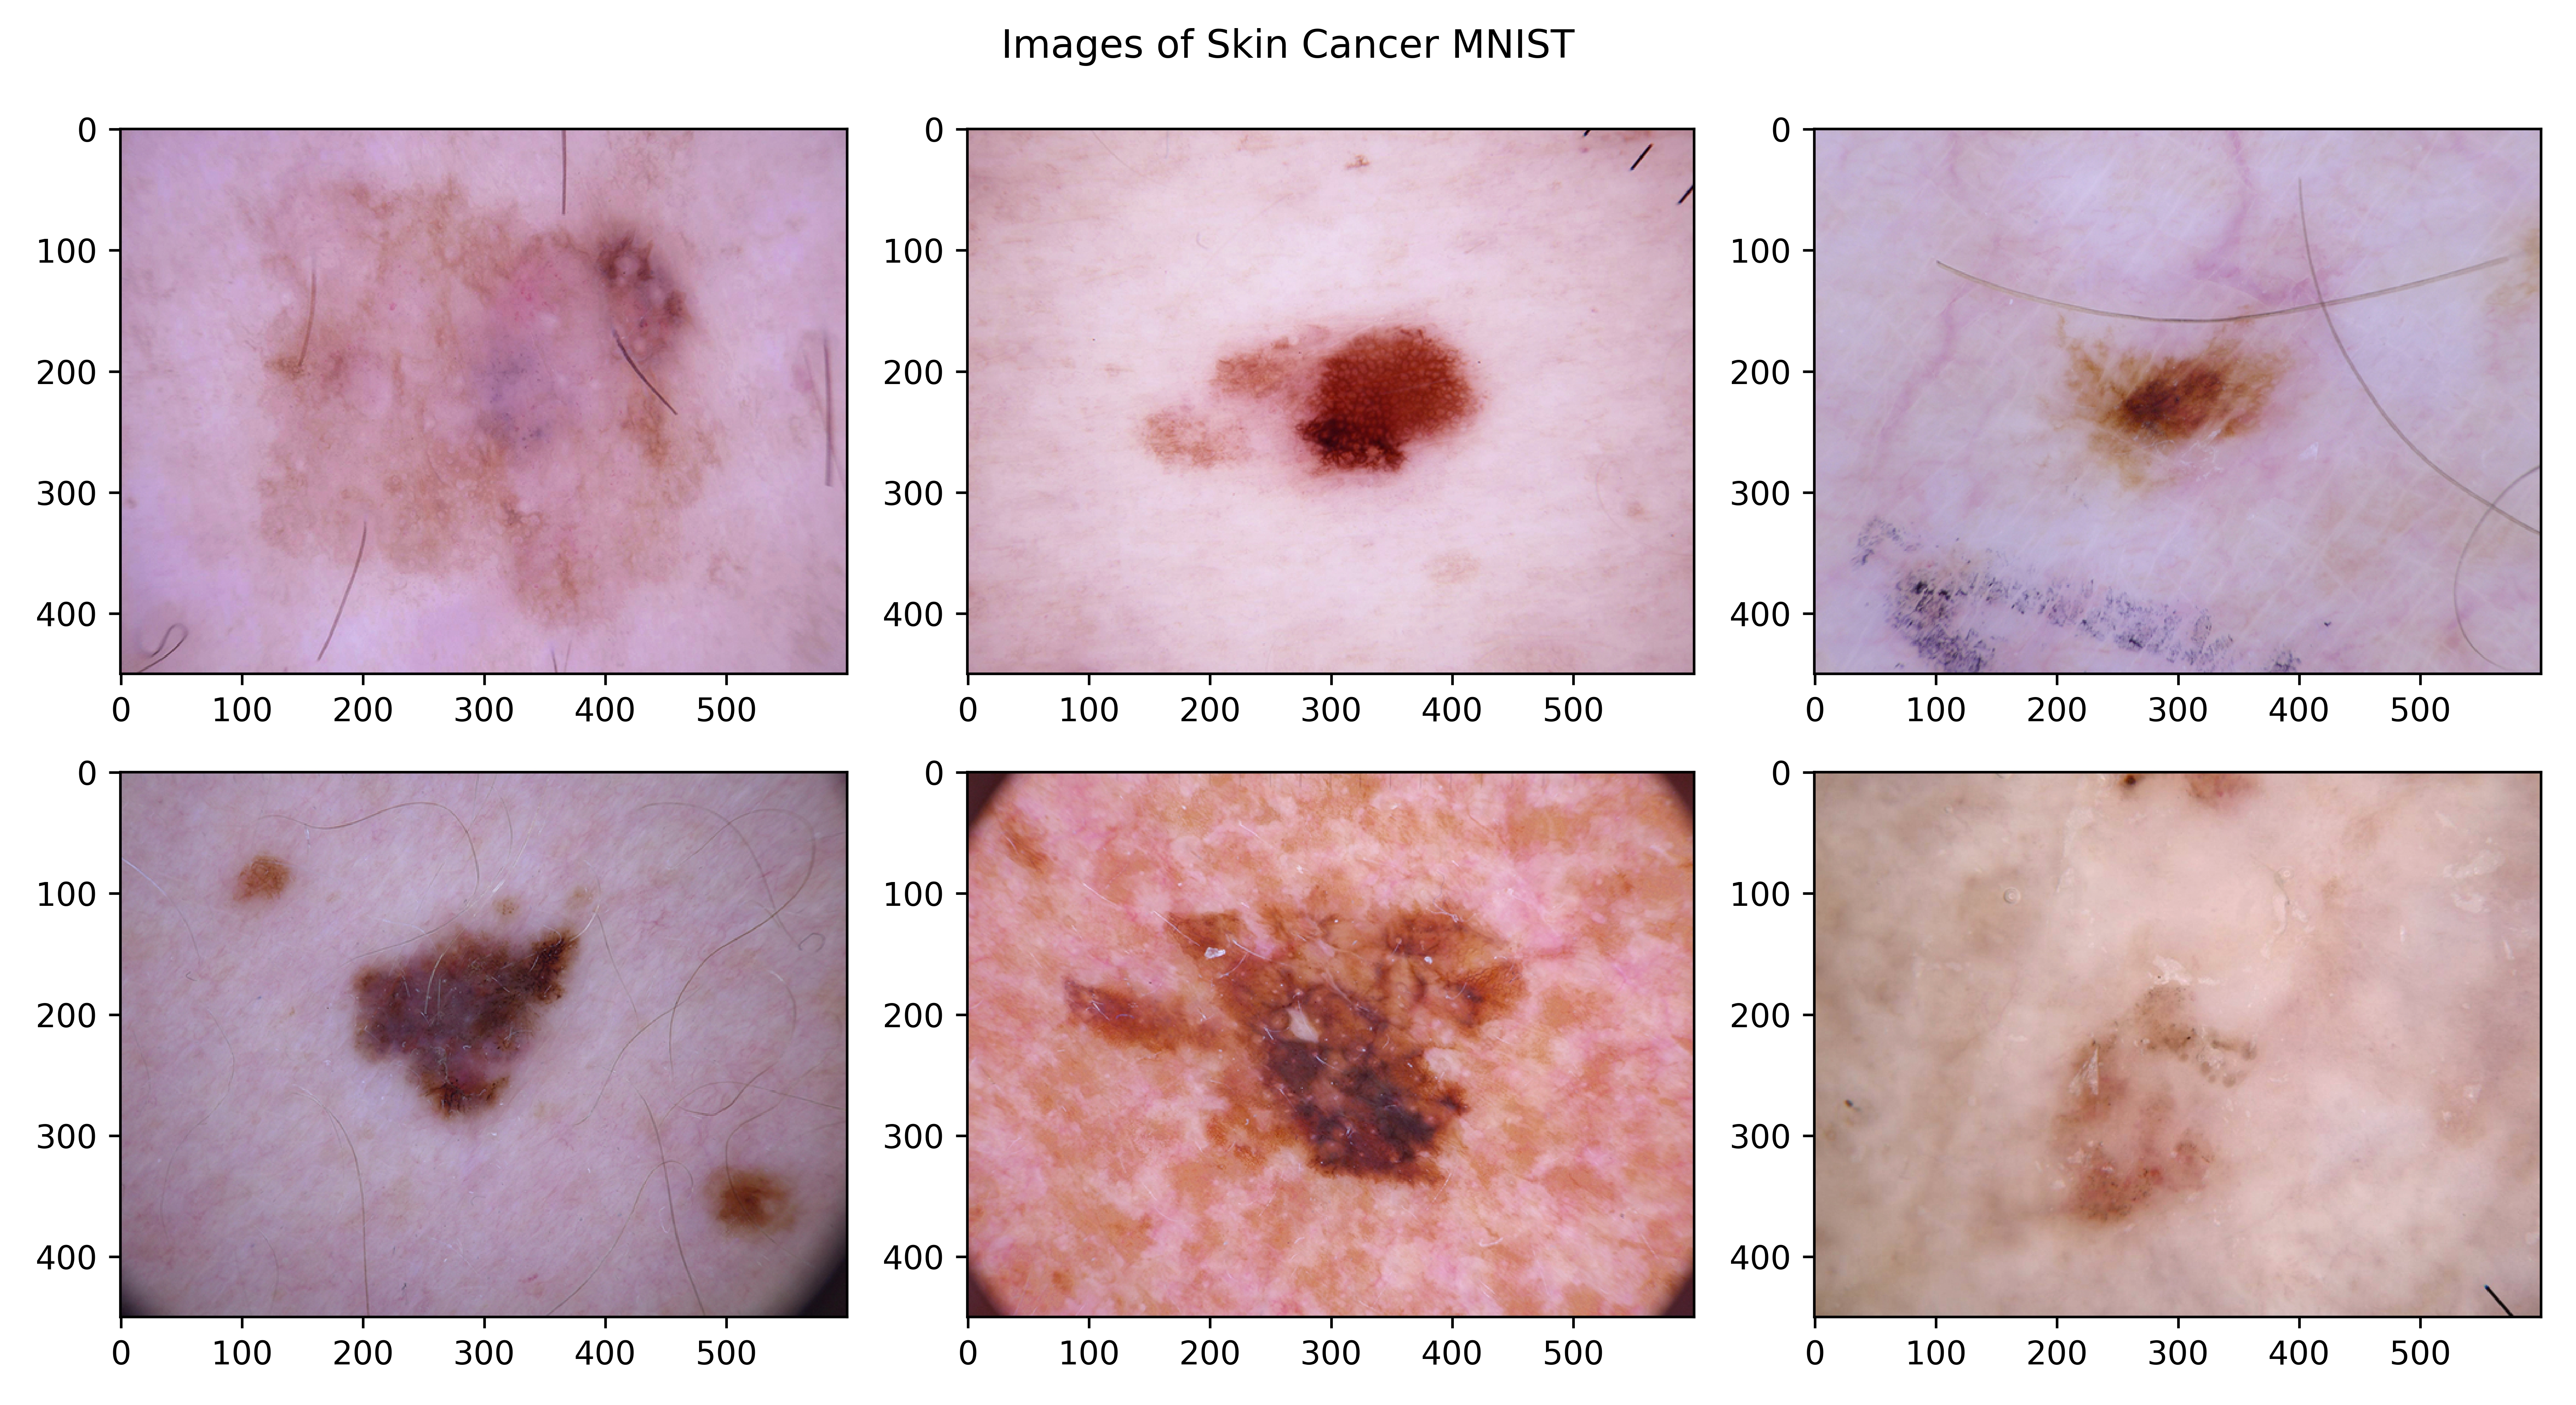
\includegraphics[width=0.9\columnwidth]{image/chap04/img401.png}
	\caption{Skin Cancer MNIST数据集示例}
	\label{img401}
\end{figure}

\section{k-wave的介绍与k空间伪谱法}
k-Wave是MATLAB的开源声学工具箱。该软件基于k空间伪谱法能实现复杂组织在真实介质中的声学仿真,并且还实现了多种对光声成像的重建方法。本项目采用该库实现对皮肤癌图像的光声成像仿真与重建。

\section{训练数据的生成与预处理}
下面介绍使用Skin Cancer MNIST数据集与k-Wave中的光声成像仿真与重建算法生成训练集与测试集的具体操作流程。

\subsection{在仿真前对Skin Cancer MNIST中的皮肤癌图像进行预处理}

\begin{enumerate}
	\item 读取图片并转为灰度图。
	\item 将图像归一化。由于用k-Wave进行模拟时外围填充的像素一定得是0,所以要在数据归一化的时候把原图里正常皮肤的部分对应到0。因此,取原图边界上的一些像素的平均值作为正常皮肤对应的像素值大小。然后在图像上将这个平均值映射到0;再在图像外围补上0像素点。
	\item 将图像降低分辨率(分辨率降低为原来的二分之一)。降采样的目的是使图像的分辨率变低,有效控制仿真的时间。
	\item 将图像的外围填充一圈0,目的是确保在光声成像模拟时,皮肤病灶完全位于圆形传感器阵列之中,使得光声成像模拟结果更加精确。
\end{enumerate}

下面选取Skin Cancer MNIST数据集中的一副皮肤癌图像对上述过程进行演示,如图\ref{img402}所示。

\begin{figure}[h]
	\centering
	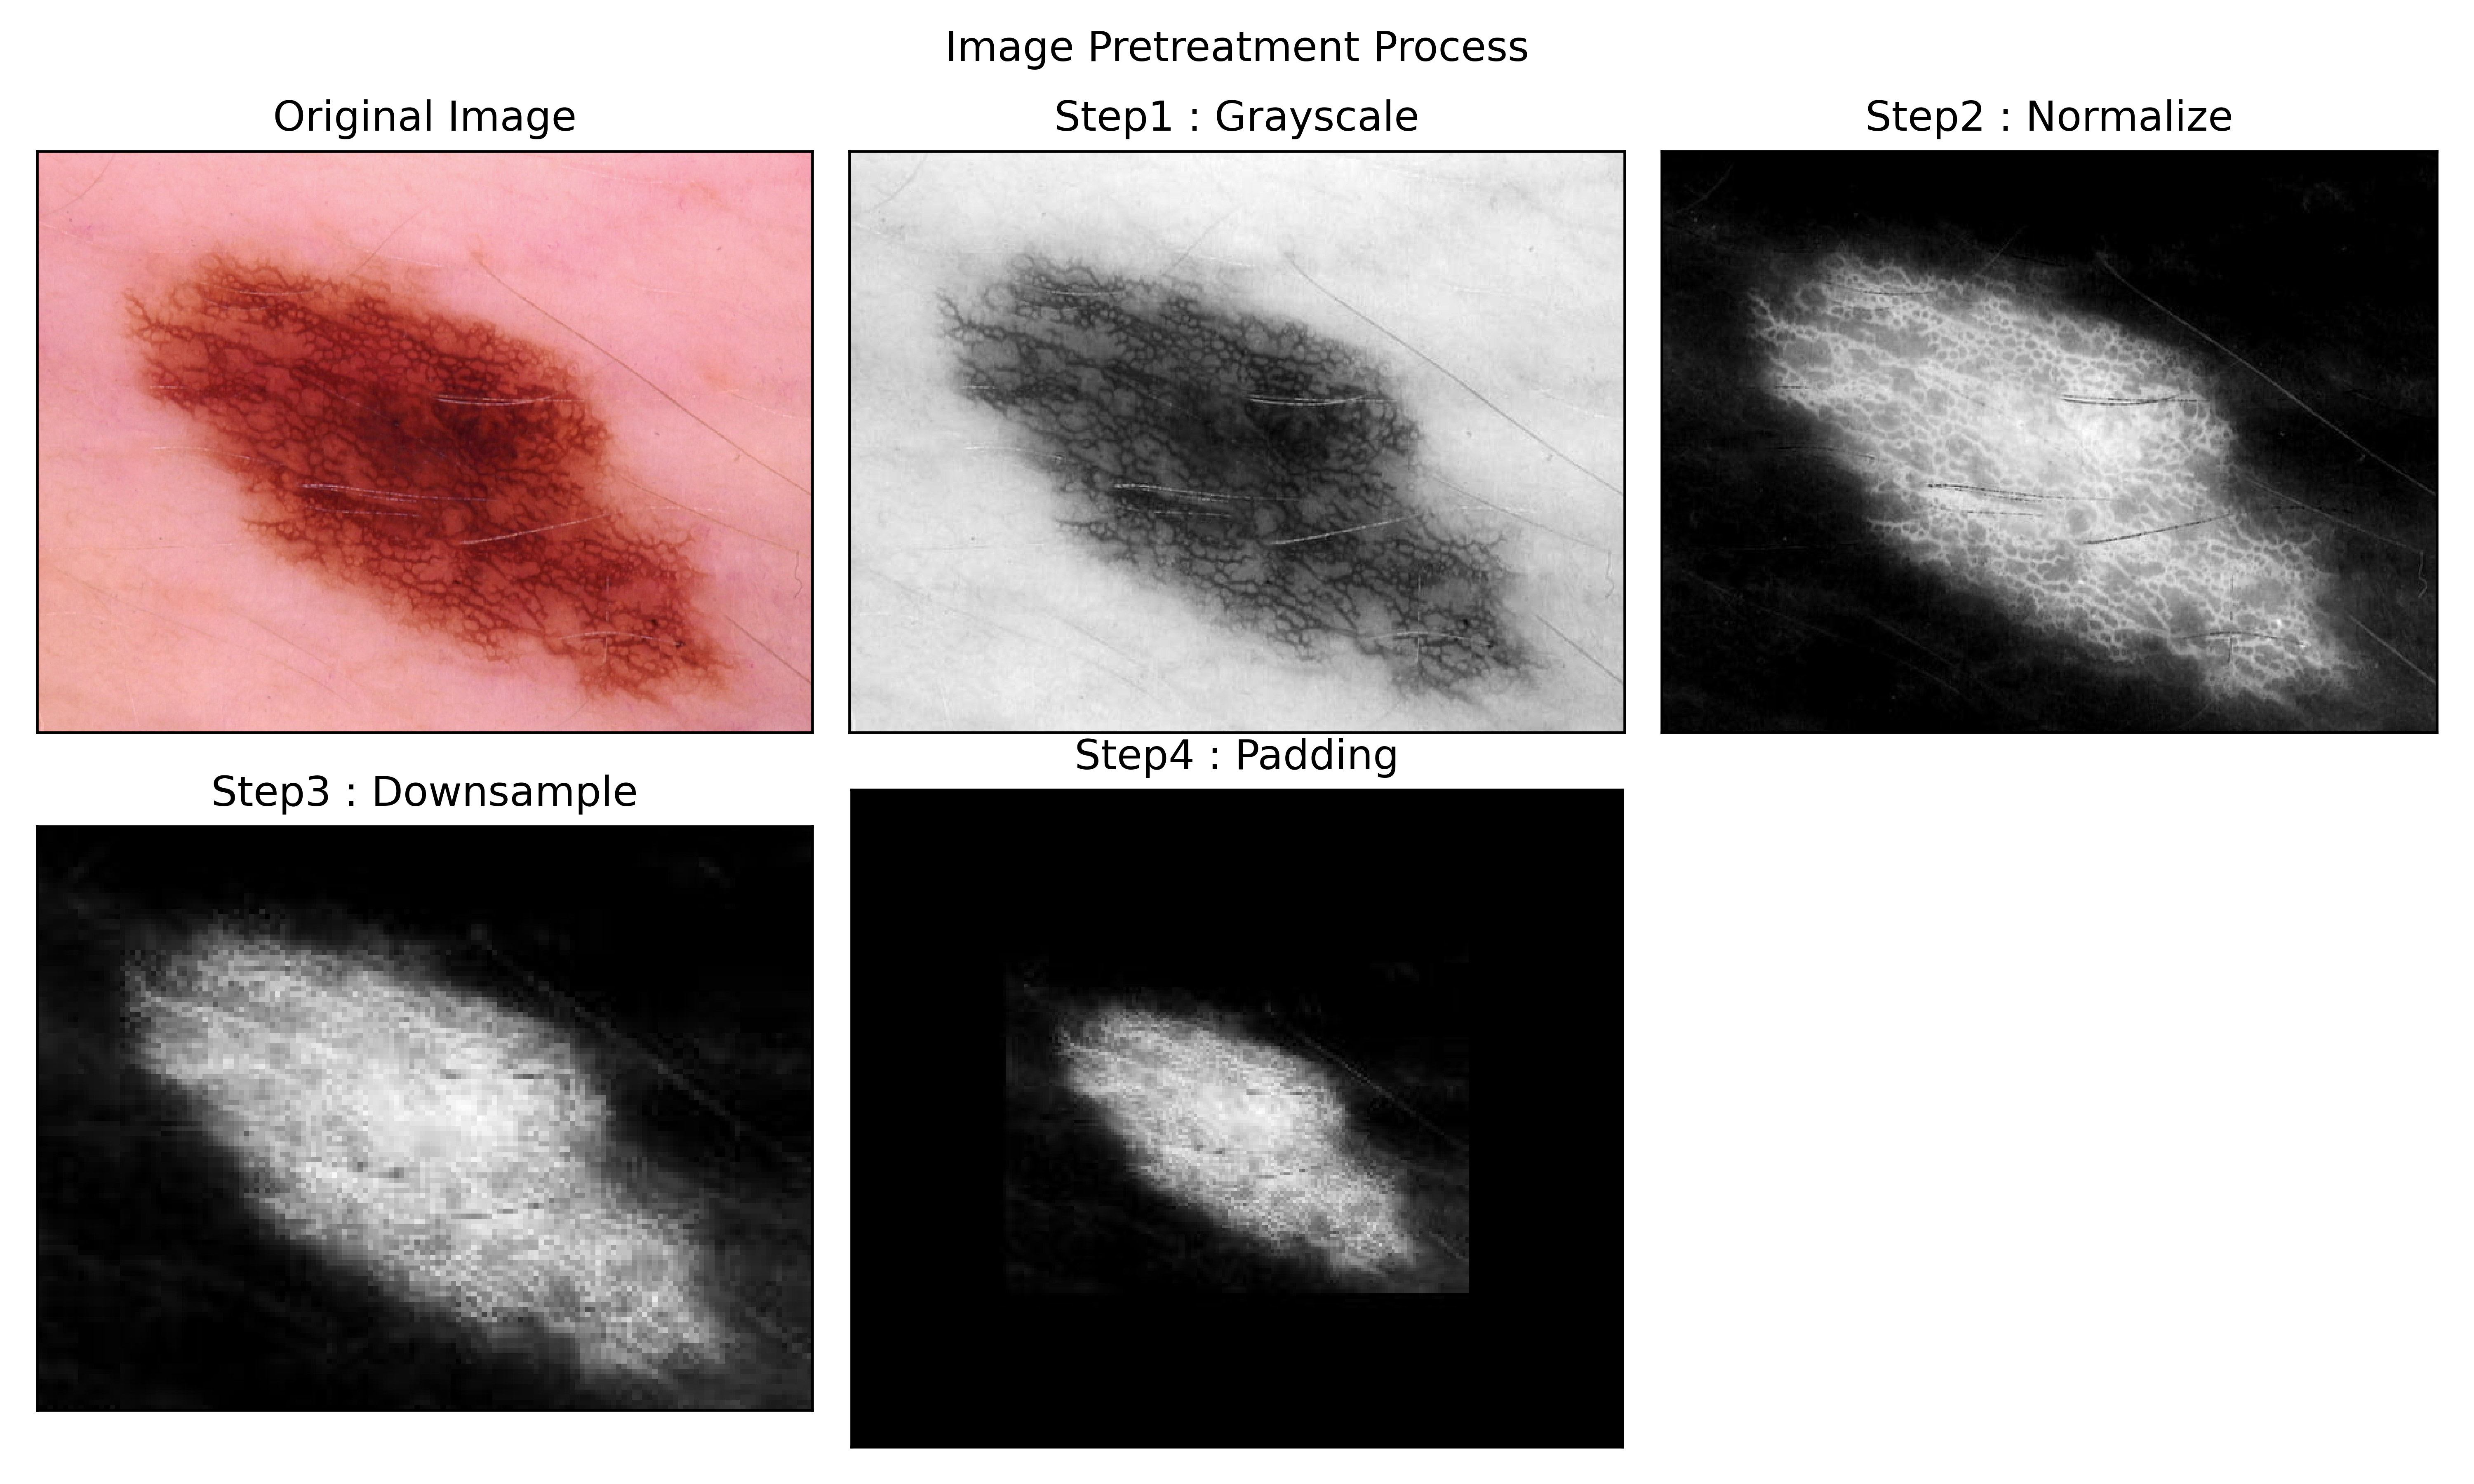
\includegraphics[width=0.9\columnwidth]{image/chap04/img402.png}
	\caption{预处理操作流程}
	\label{img402}
\end{figure}

\subsection{利用k-Wave对预处理后的图像进行光声成像仿真}
首先需要初始化k-Wave进行光声成像仿真各参数。在使用k-Wave进行光声成像模拟前,要设置的参数如图\ref{img403}所示。

\begin{figure}[h]
	\centering
	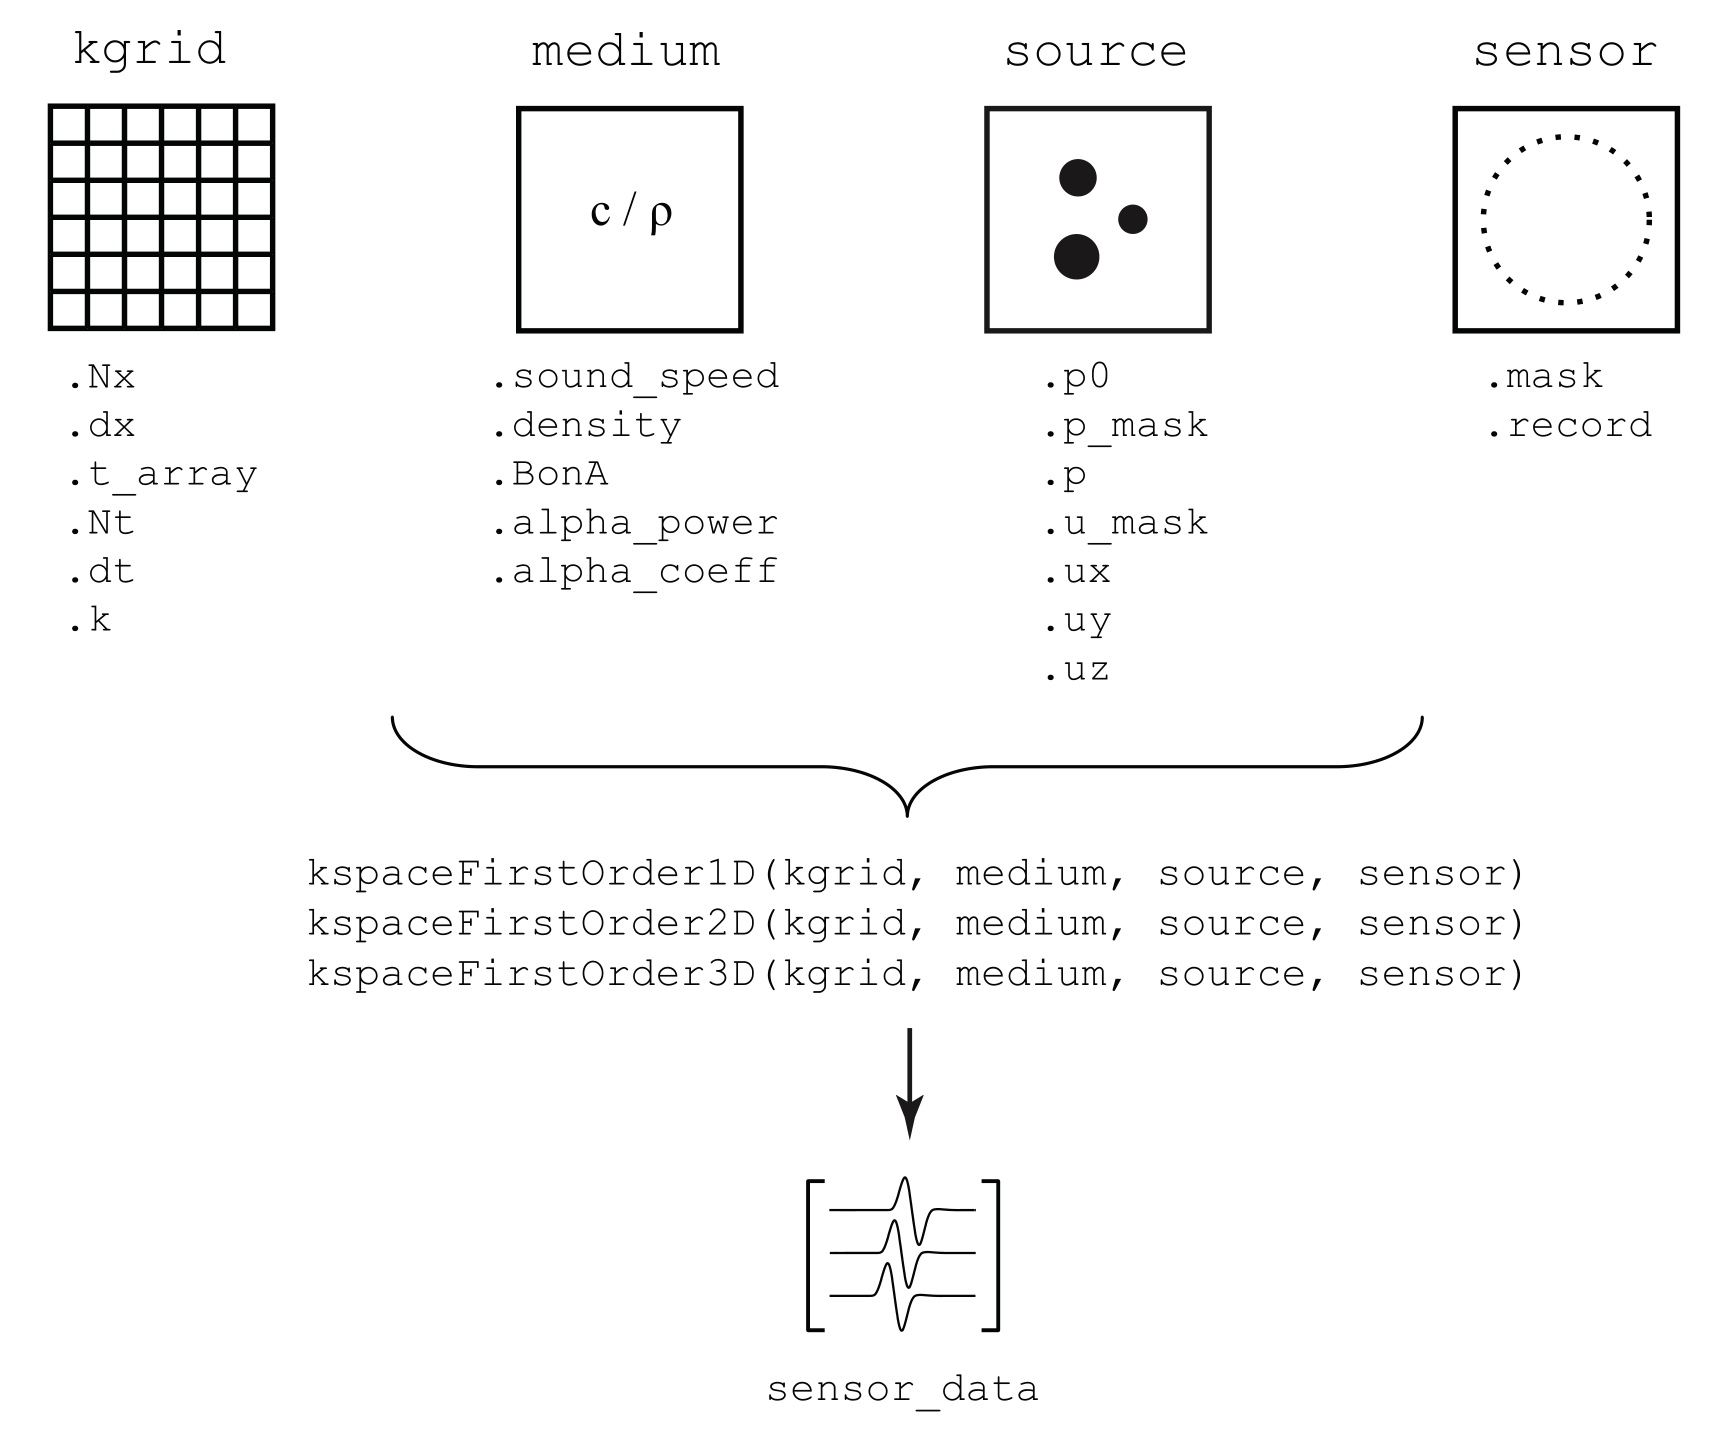
\includegraphics[width=0.6\columnwidth]{image/chap04/img403.png}
	\caption{k-Wave仿真的设置参数\cite{treeby2010k}}
	\label{img403}
\end{figure}
即创建计算网格、定义介质属性、定义初始压力、定义传感器掩模。

\begin{enumerate}
	\item 其中由于查资料得知:人体软组织声速接近1540m/s;2006年全国男人人体密度=$1.0913-0.0016\cdot (10.8+15.8)=1.0487\cdot 10^3kg/(m^3)$、女人人体密度=$1.0897-0.00133\cdot (17.5+17.5)=1.0431\cdot 10^3kg/(m^3)$。于是我设置介质声速为人体软组织声速,将男人人体密度与女人人体密度的平均值设置为介质密度。
	\item 将预处理好的图片导入模型中作为初始压力分布。
	\item 定义具有50个传感器元件的中心圆的笛卡尔传感器掩模
\end{enumerate}
在设置完如上参数后,利用MatLab运行kwave仿真。得出的输出数据senser data是形状为$[num\ sensor,time\ step]$的矩阵,记录了各传感器在各时间步长所接收到的压力数据。将其运用Matlab中的images函数做出图\ref{img404}。图片每一行代表着一个传感器在仿真过程中所接收到的压力的大小变化。

\begin{figure}[h]
	\centering
	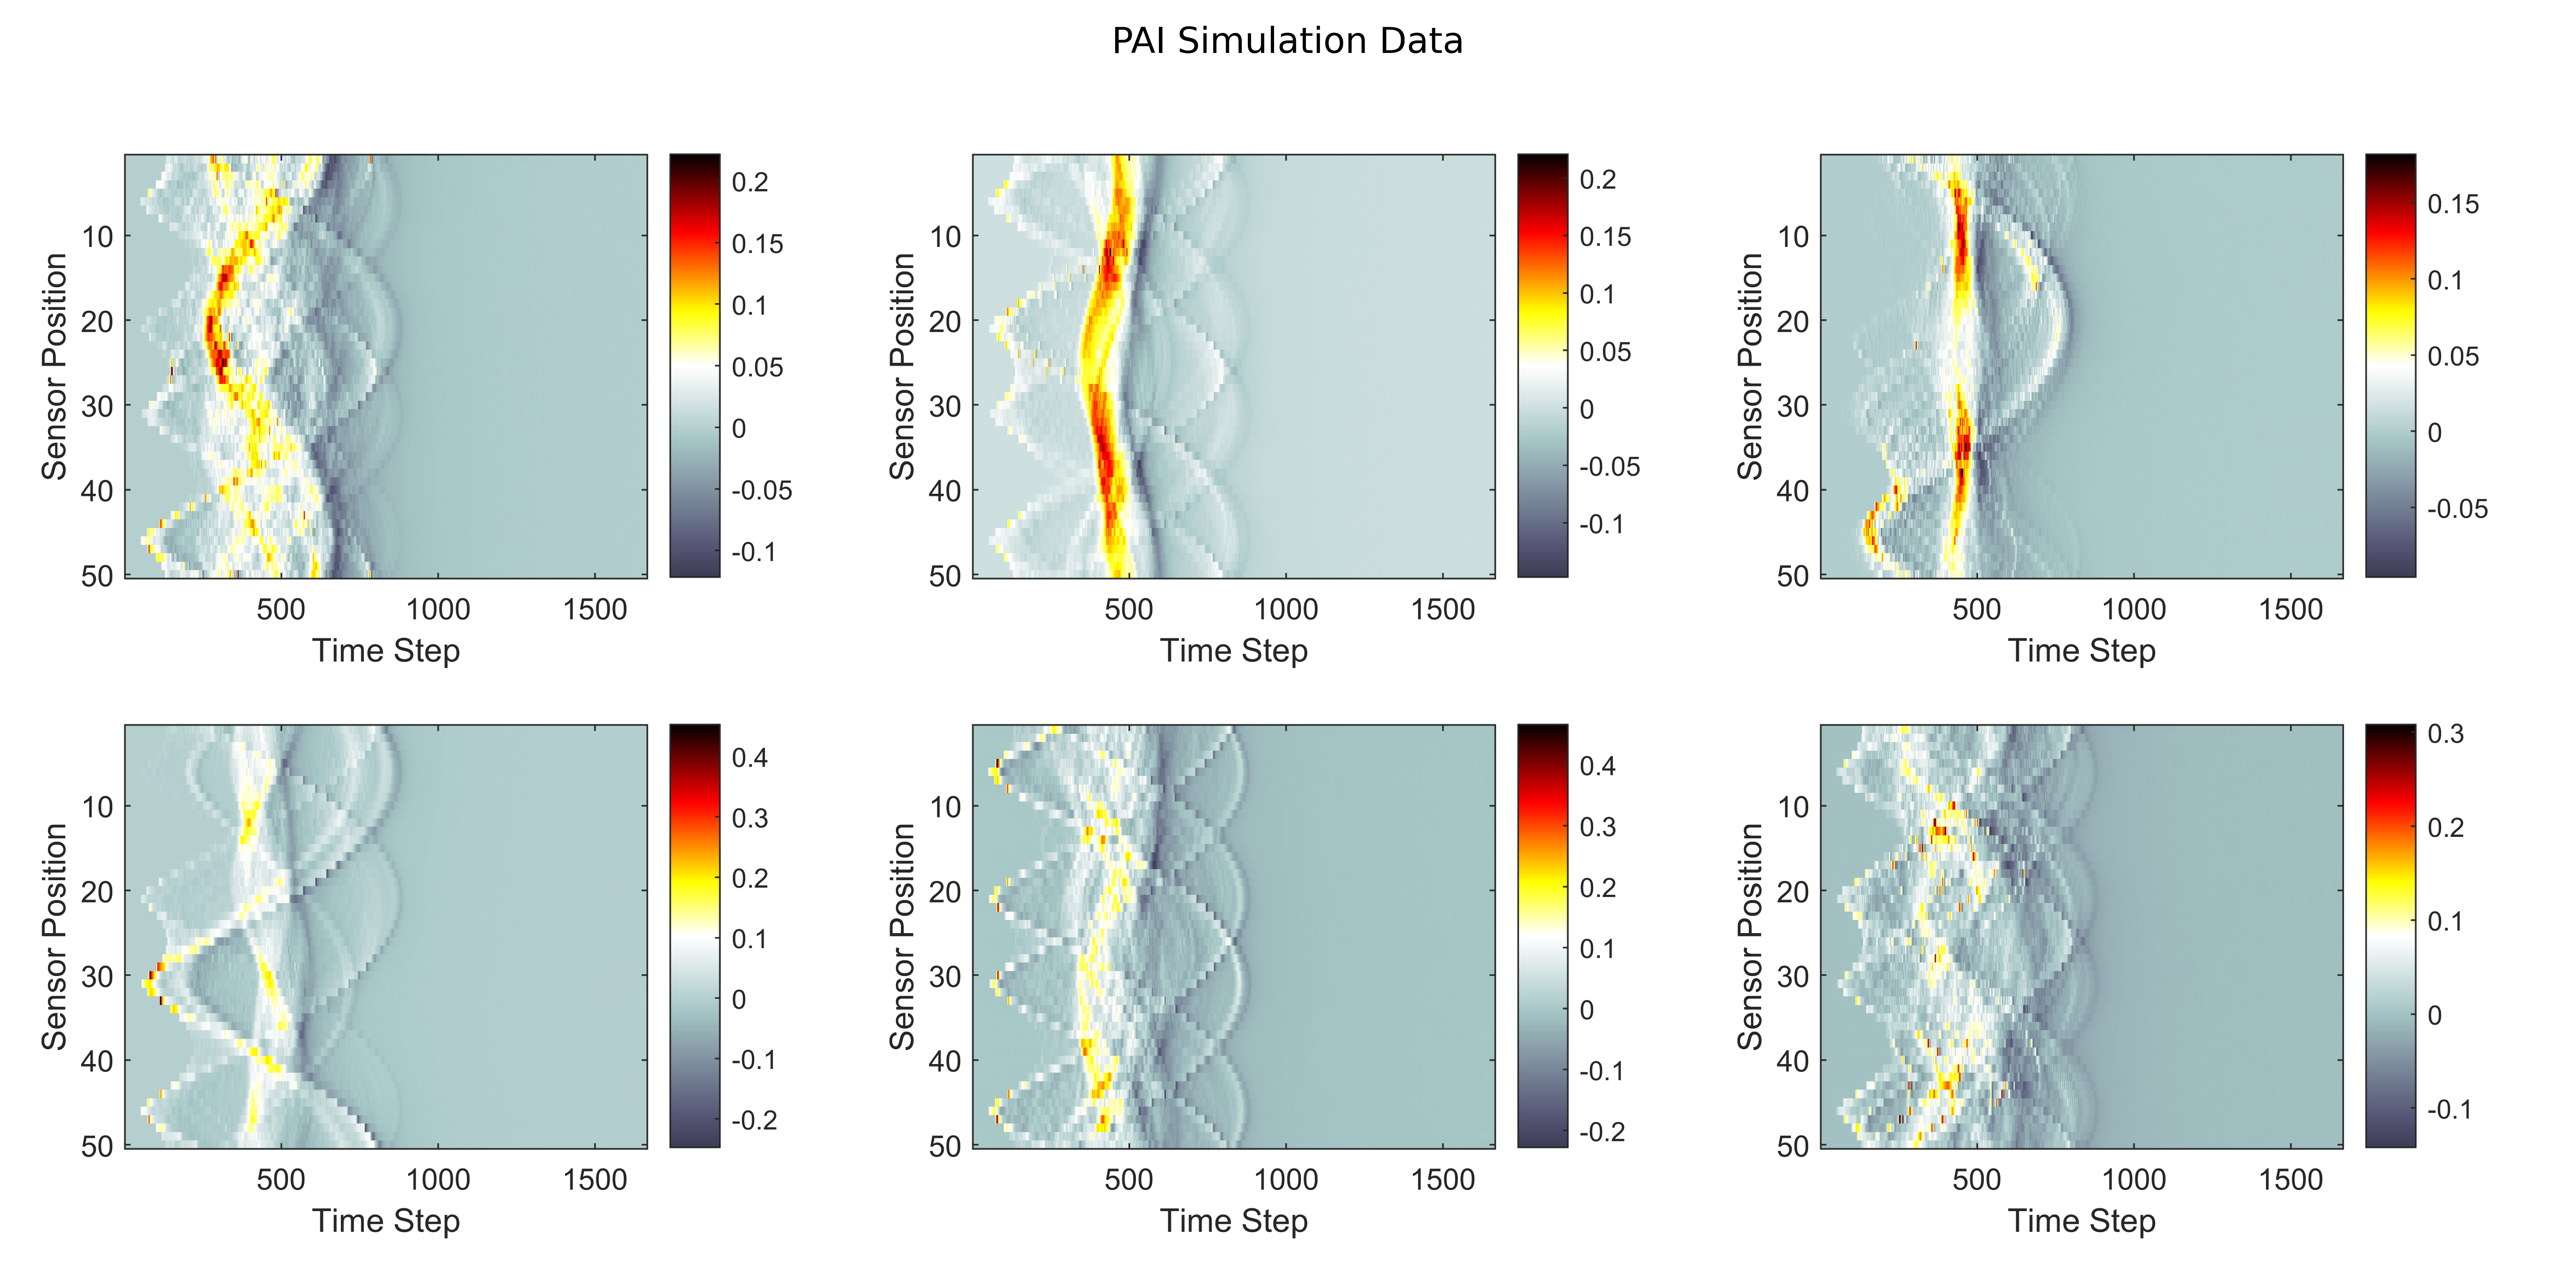
\includegraphics[width=0.9\columnwidth]{image/chap04/img404.png}
	\caption{光声传感器接收到的压力数据示例}
	\label{img404}
\end{figure}

\subsection{进行光声成像的重建得到训练数据}
在进行光声成像重建前,同样需要初始化k-Wave的各项参数,并且确保其与仿真时保持一致;然后才能使用k-Wave中的相关函数进行光声成像的重建。重建图像如图所示\ref{img405}。其中左侧为原图像,右侧为相应的重建图像。

\begin{figure}[h]
	\centering
	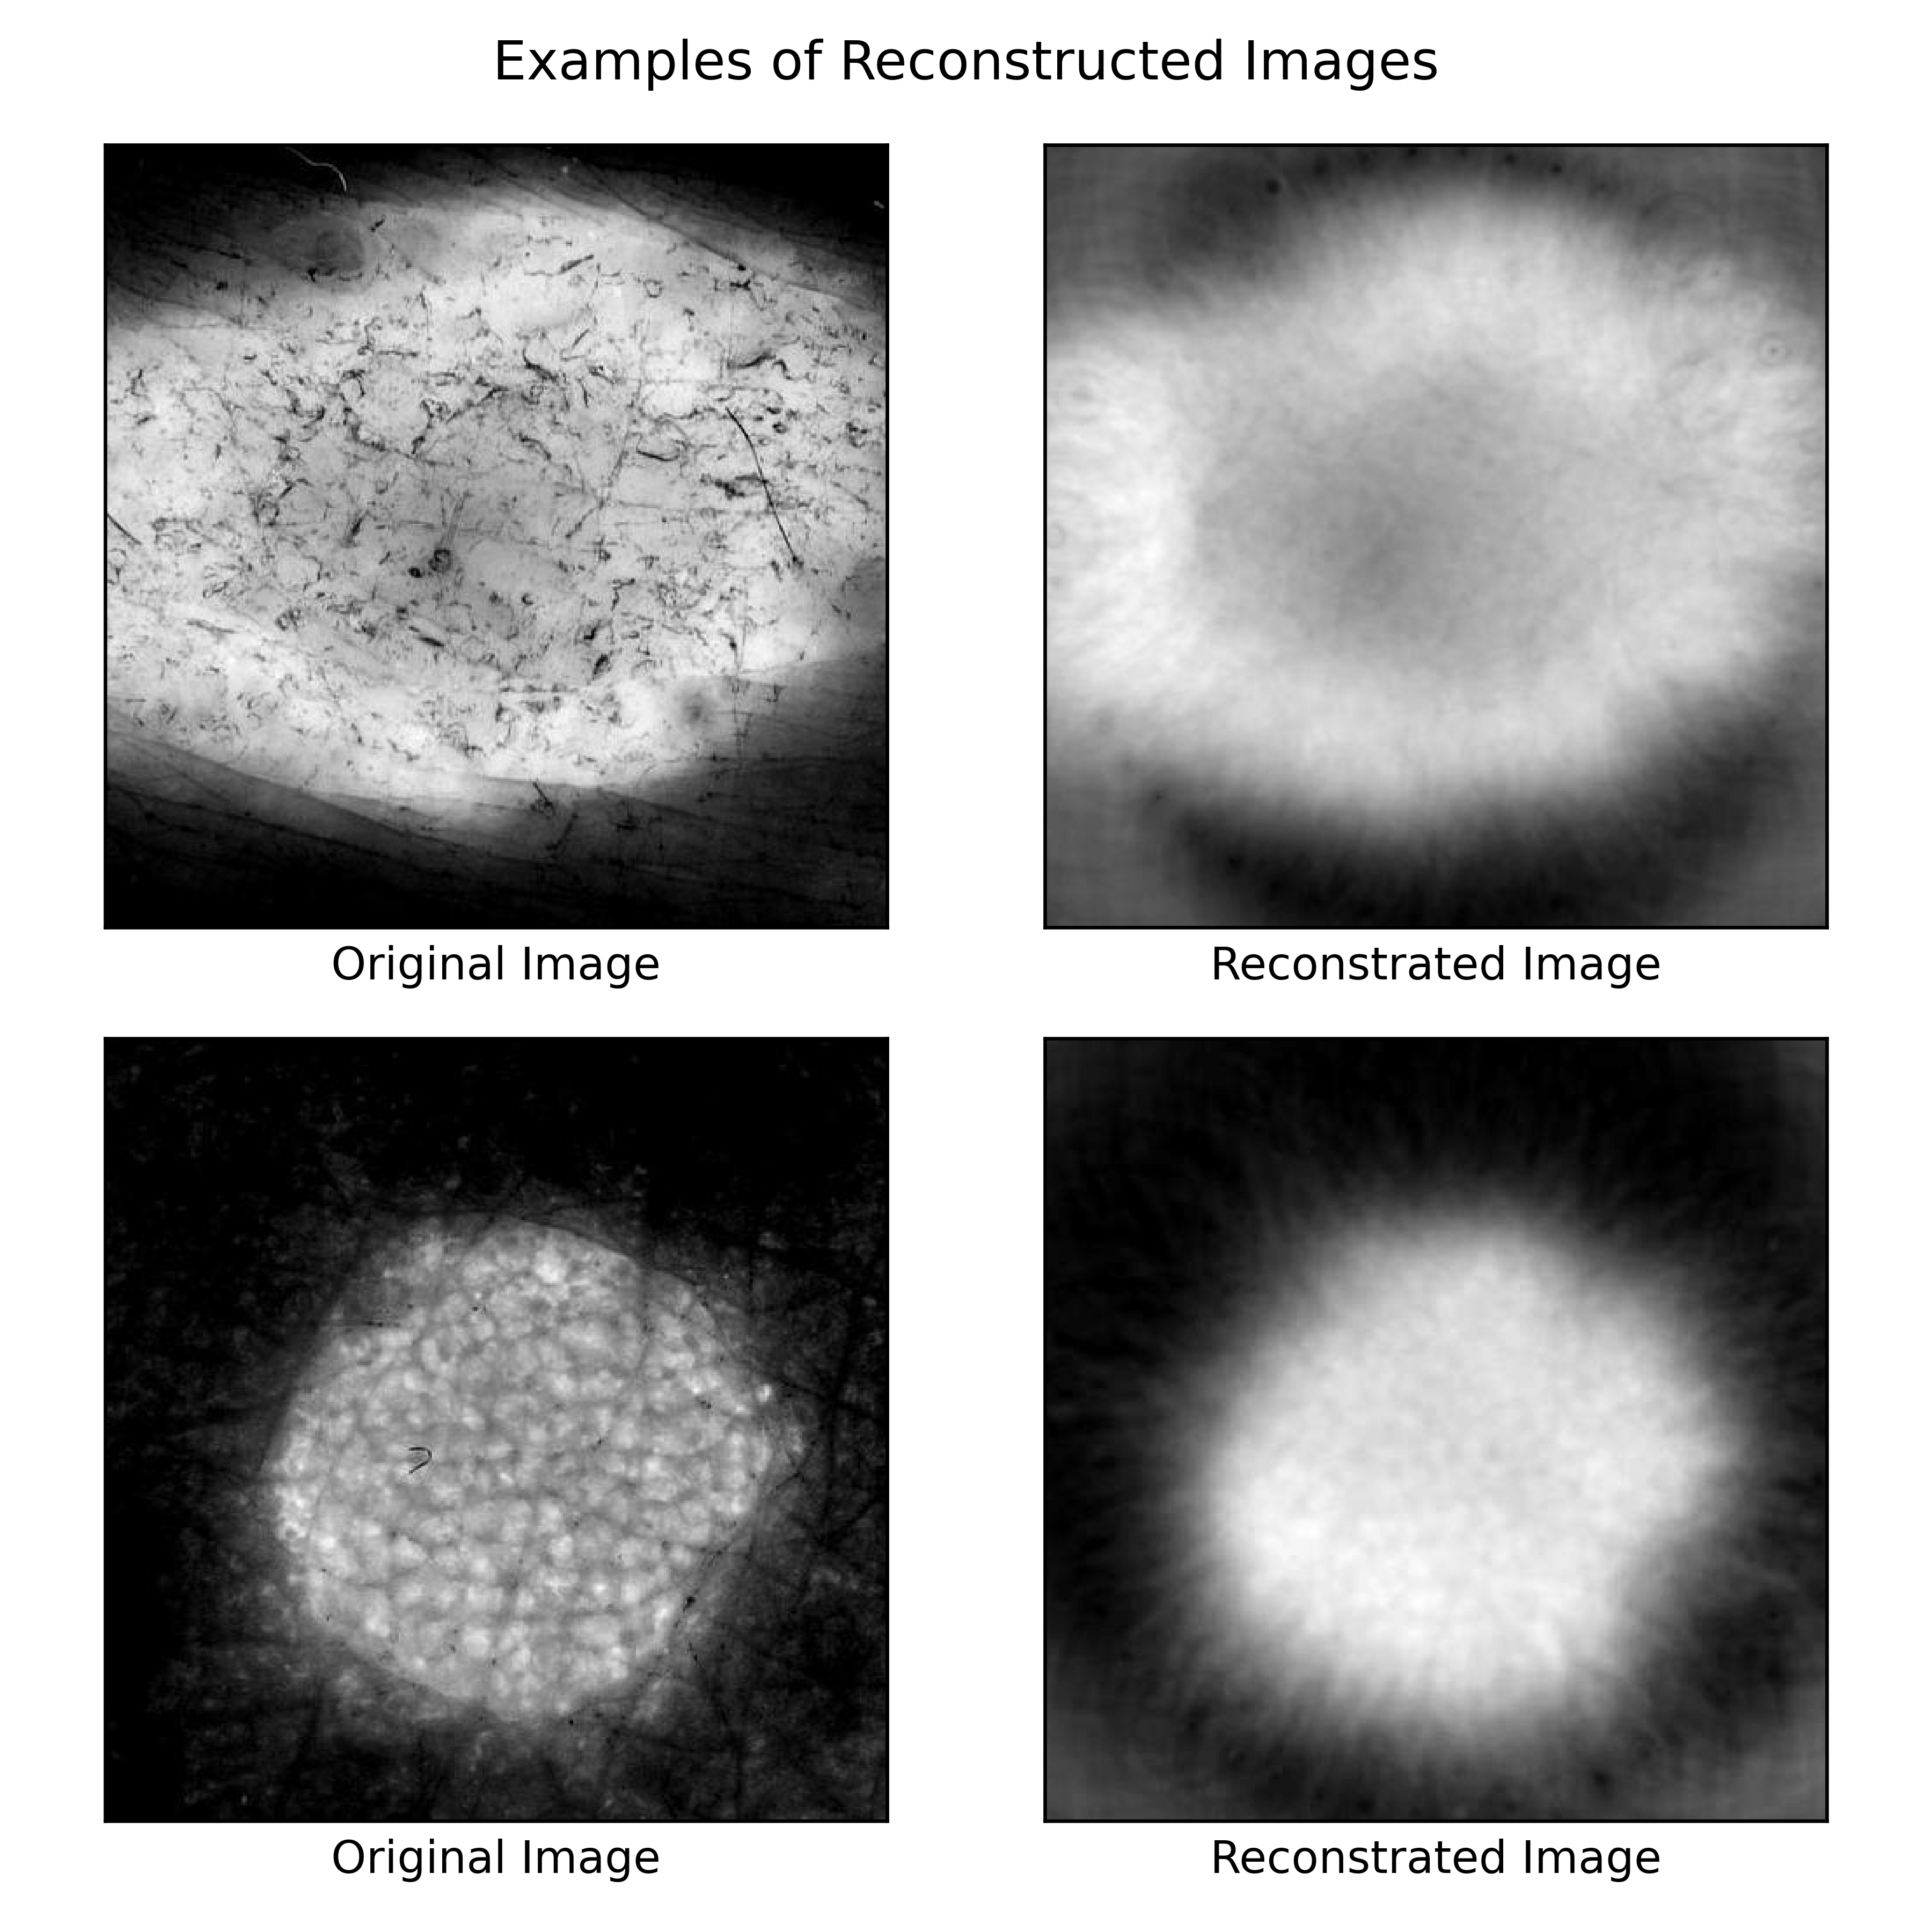
\includegraphics[width=0.75\columnwidth]{image/chap04/img405.png}
	\caption{重建图像示例}
	\label{img405}
\end{figure}

\subsection{将得到的数据集划分成训练集及测试集}
经过上述光声成像仿真与重建,最终共得到6000张重建图像。将其中的5000张重建图像及其原图像划分为训练集,将其余的1000张重建图像及其原图像划分为测试集。
\newclearpage
\section{总结与展望}
\subsection*{总结与展望}
\frame{
	\footnotesize
	\begin{block}{工作总结}
		\begin{itemize}
			\item[\dag] 本文的模型结合了卷积网络的特征学习能力与长短记忆网络对整体局部建模的能力,相比于全卷积网络,大幅度地提高了了模型性能
			\item[\dag] 大量的对比实验与结果分析证明了模型的有效性
		\end{itemize}
	\end{block}
	\vspace{-1em}
	\begin{block}{展望}
		\begin{itemize}
			\item[\dag] 模型性能:提高网络的深度来学习更高层次的特征,提高模型效果(He et al. ResNet, CVPR 2016)
			\item[\dag] 模型大小:通过裁剪网络冗余部分(Han et al. Deep Compression, ICLR 2016 Best Paper)或使用二值网络减少模型参数(Courbariaux et al. Binaryconnect, NIPS 2015)
			\item[\dag] 训练数据:使用无监督或弱监督的方式训练网络(Papandreou et al. Weakly-and semi-supervised learning, ICCV 2015)
		\end{itemize}
	\end{block}
}



\newclearpage
%% chapter 4 dataset, network structure, experiment and result
\chapter{模型的分析与评估}
\label{cha:experiment}

将验证集中的1000张重建图像输入已训练的模型,得到重建图像的预测图像后,计算预测图象与原图像的MSE、PSNR、SSIM等评价指标,并对比重建图像与原图像之间的MSE、PSNR、SSIM等值,对模型的优化效果进行分析与评估。

\section{MSE}

\subsection{MSE简介}
MSE是衡量两张图片的相似程度的一种常见方法。两个图片之间的MSE即求两张图片各个相对应的像素点的平方差之和的均值。具体公式如下:

\begin{equation} \label{601}
	MSE(I,K)=\cfrac{1}{mn}\sum_{i=0}^{m-1}\sum_{j=0}^{n-1}\big [I(i,j)-K(i,j)]^2
\end{equation}

\subsection{使用MSE衡量模型效果}
计算验证集中的1000张重建图像与原图像的MSE值和预测图像与原图像的MSE值,结果如图\ref{fig601}所示。
 
\begin{figure}[h]
	\centering
	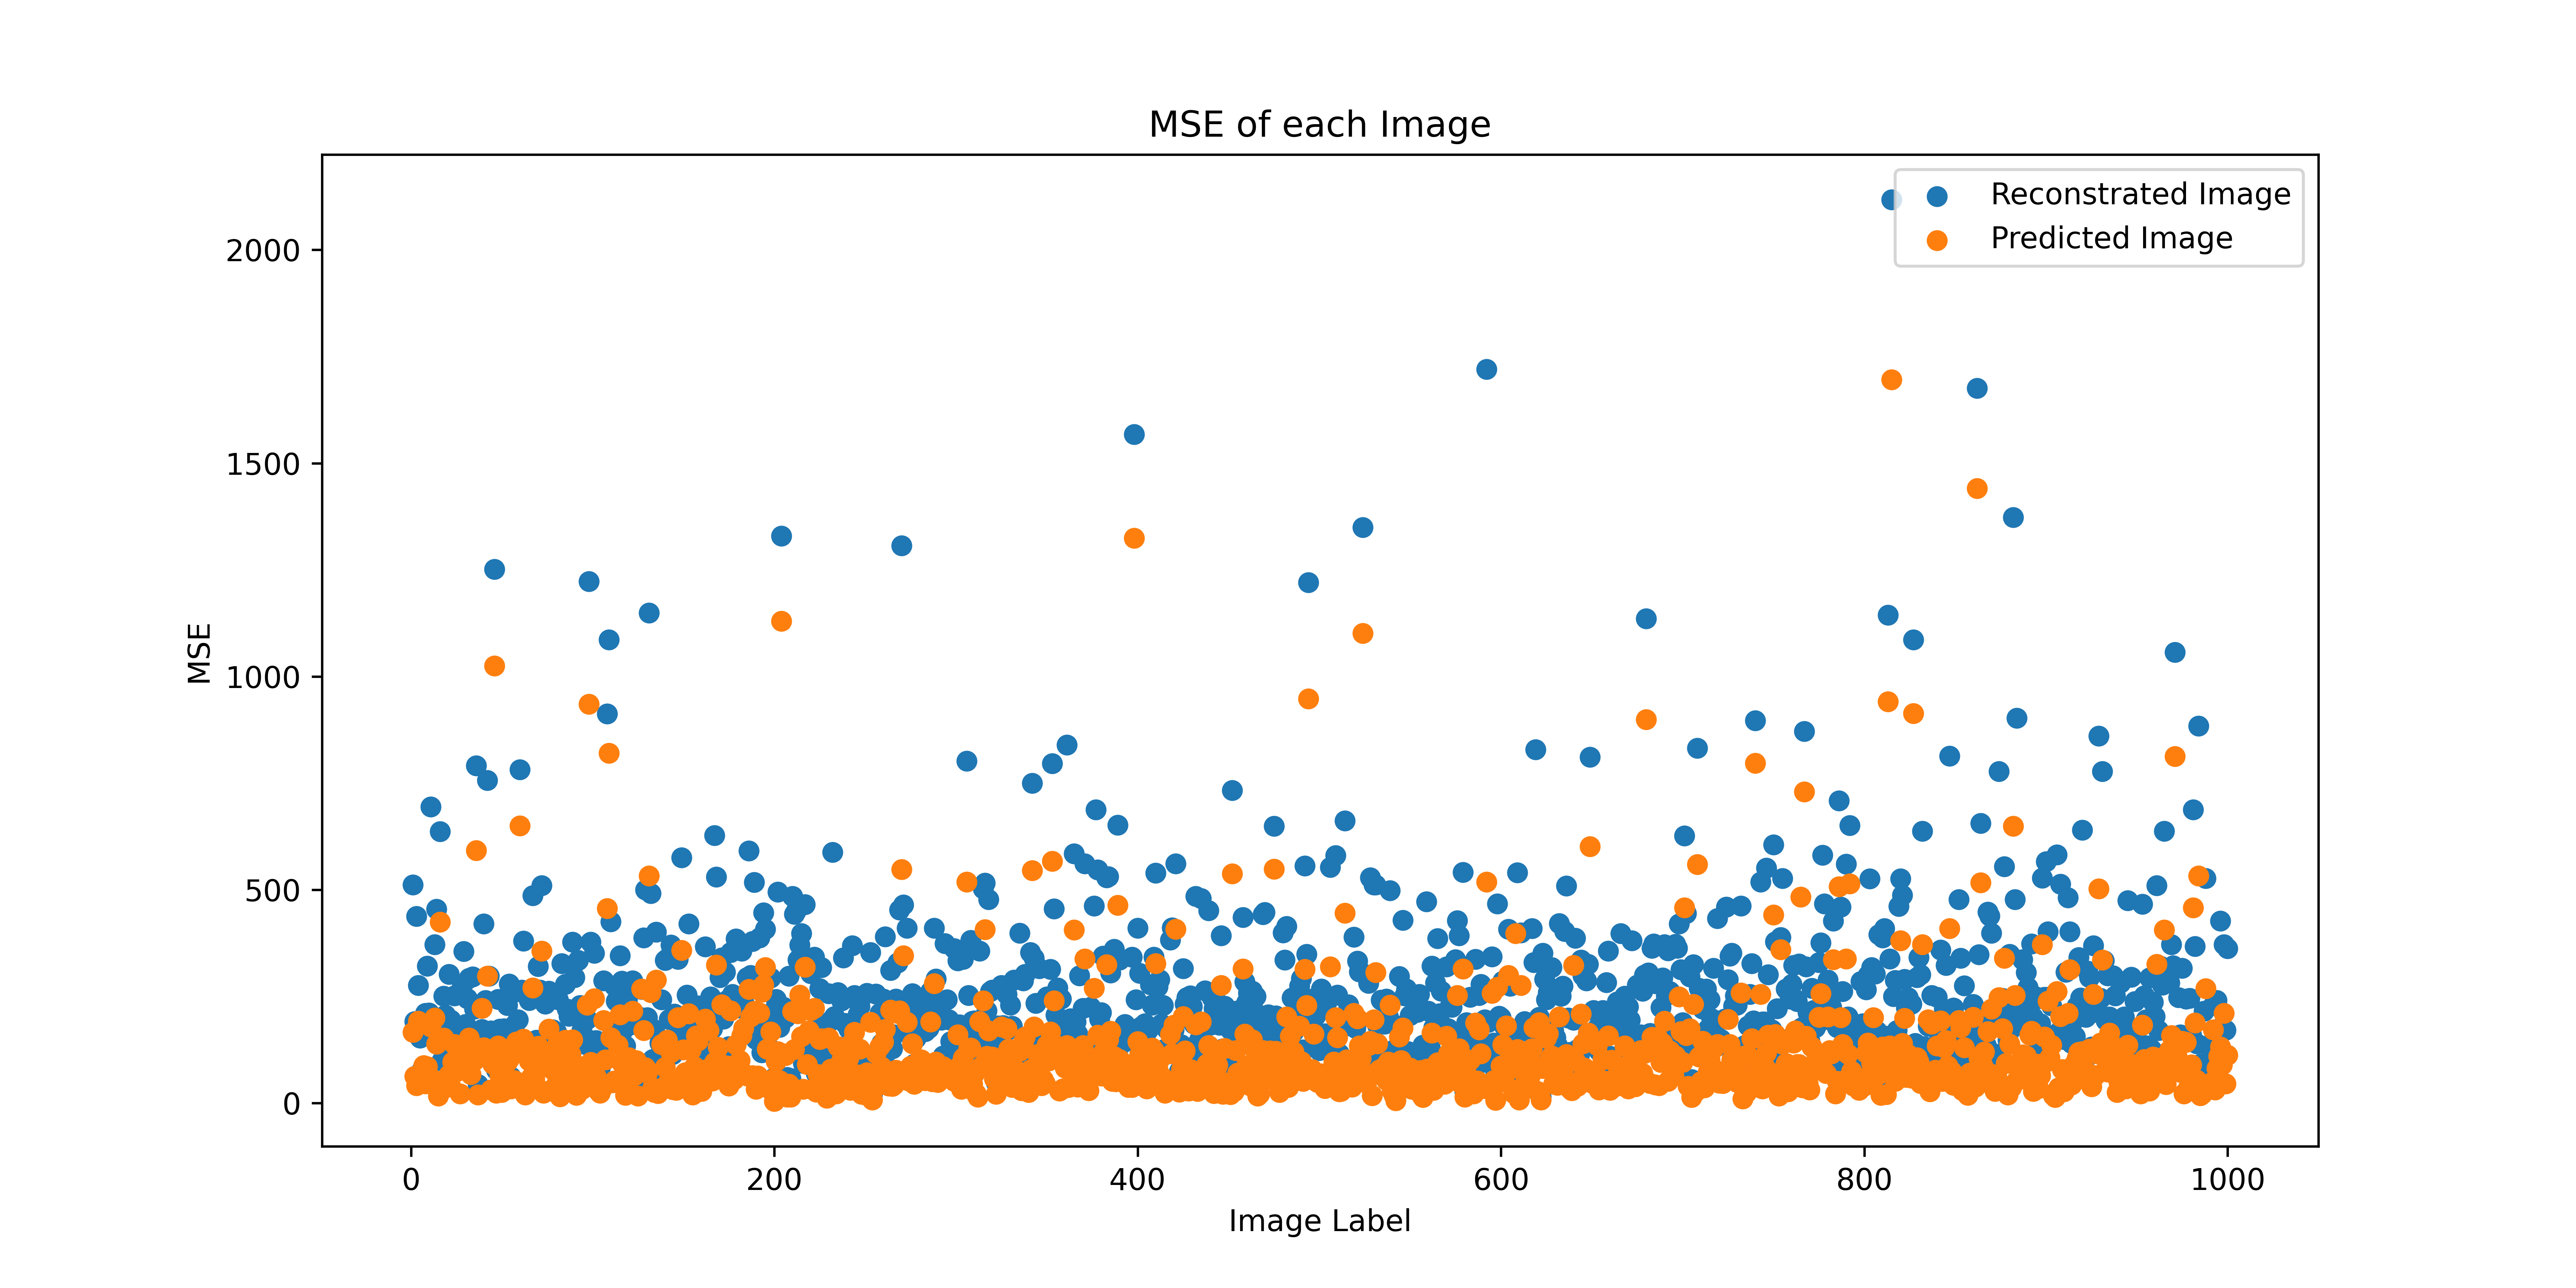
\includegraphics[width=0.9\columnwidth]{image/chap06/img601.png}
	\caption{测试集图像及其预测图象与原图像的MSE}
	\label{fig601}
\end{figure}

在图\ref{fig601}中,X轴为各图像的编号,Y轴为对应的MSE值。从图\ref{fig601}可以看出,预测图象的MSE值在图中的主要分布区域为0到250,而重建图像的MSE值的主要分布区域为100到500。且在MSE值超过500的区域,重建图像的数量显著多于预测图像。进一步,计算这1000张重建图像与预测图像的MSE值的平均值,计算结果如图\ref{fig602}。

\begin{figure}[h]
	\centering
	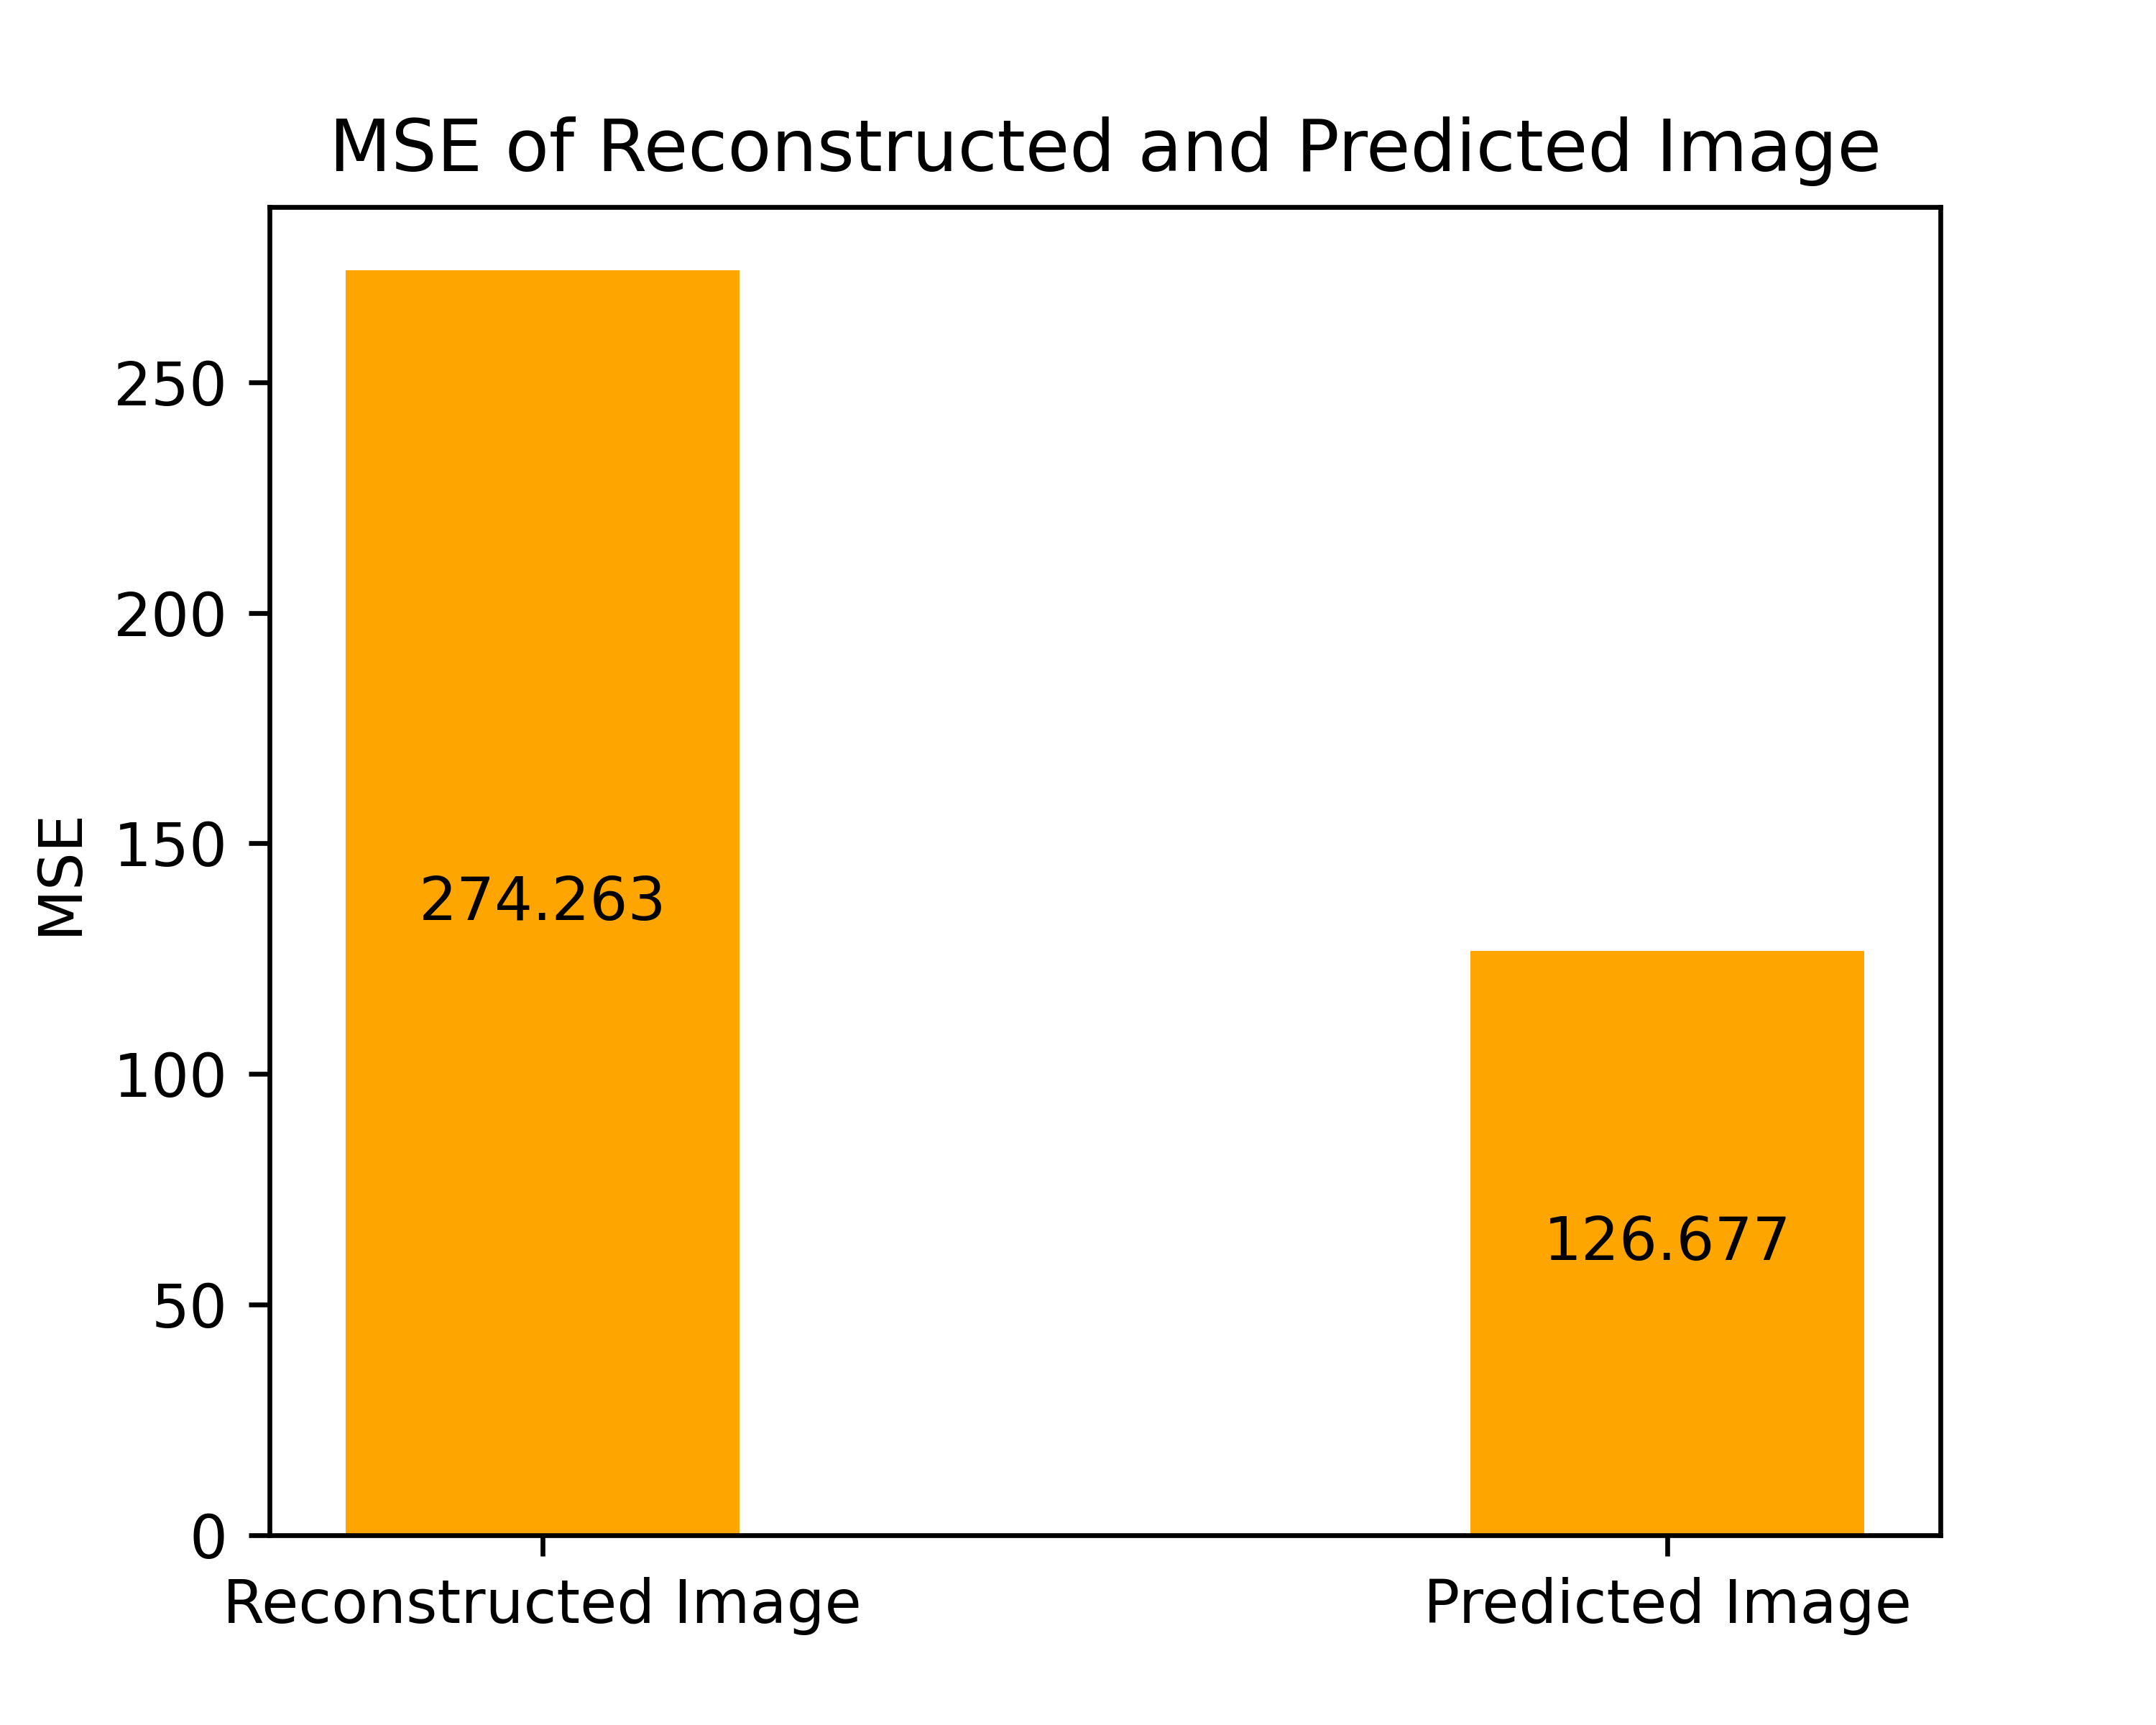
\includegraphics[width=0.75\columnwidth]{image/chap06/img602.png}
	\caption{测试集图像及其预测图象与原图像的MSE的均值}
	\label{fig602}
\end{figure}

 从图\ref{fig602}可以得出,在输入模型后所得优化图像,相比原来的重建图像,平均的MSE值由274.263下降为126.677,这说明模型对原来的重建图像具有良好的优化效果。
 
 \section{PSNR}
 \subsection{PSNR简介}
 PSNR即峰值信噪比,PSNR的计算涉及到MSE。它的公式如下:
 
 \begin{equation} \label{602}
 	\begin{aligned}
 		PSNR(I,K)=10\cdot log_{10}(\cfrac{MAX_I^2}{MSE})
 	\end{aligned}
 \end{equation}

对数内分母为均方误差MSE,分子中的$MAX_I$为最大像素值,即若为b位图像,该值为$2^b-1$。当两张图片的MSE差异越小,则对数内的值越大,此时PSNR就越大。因此,PSNR越大就表示图像相似程度越高。

\subsection{利用PSNR衡量模型效果}
 计算验证集中的1000张重建图像与原图像的PSNR值和预测图像与原图像的PSNR值,结果如图\ref{fig603}所示。
 
 \begin{figure}[h]
 	\centering
 	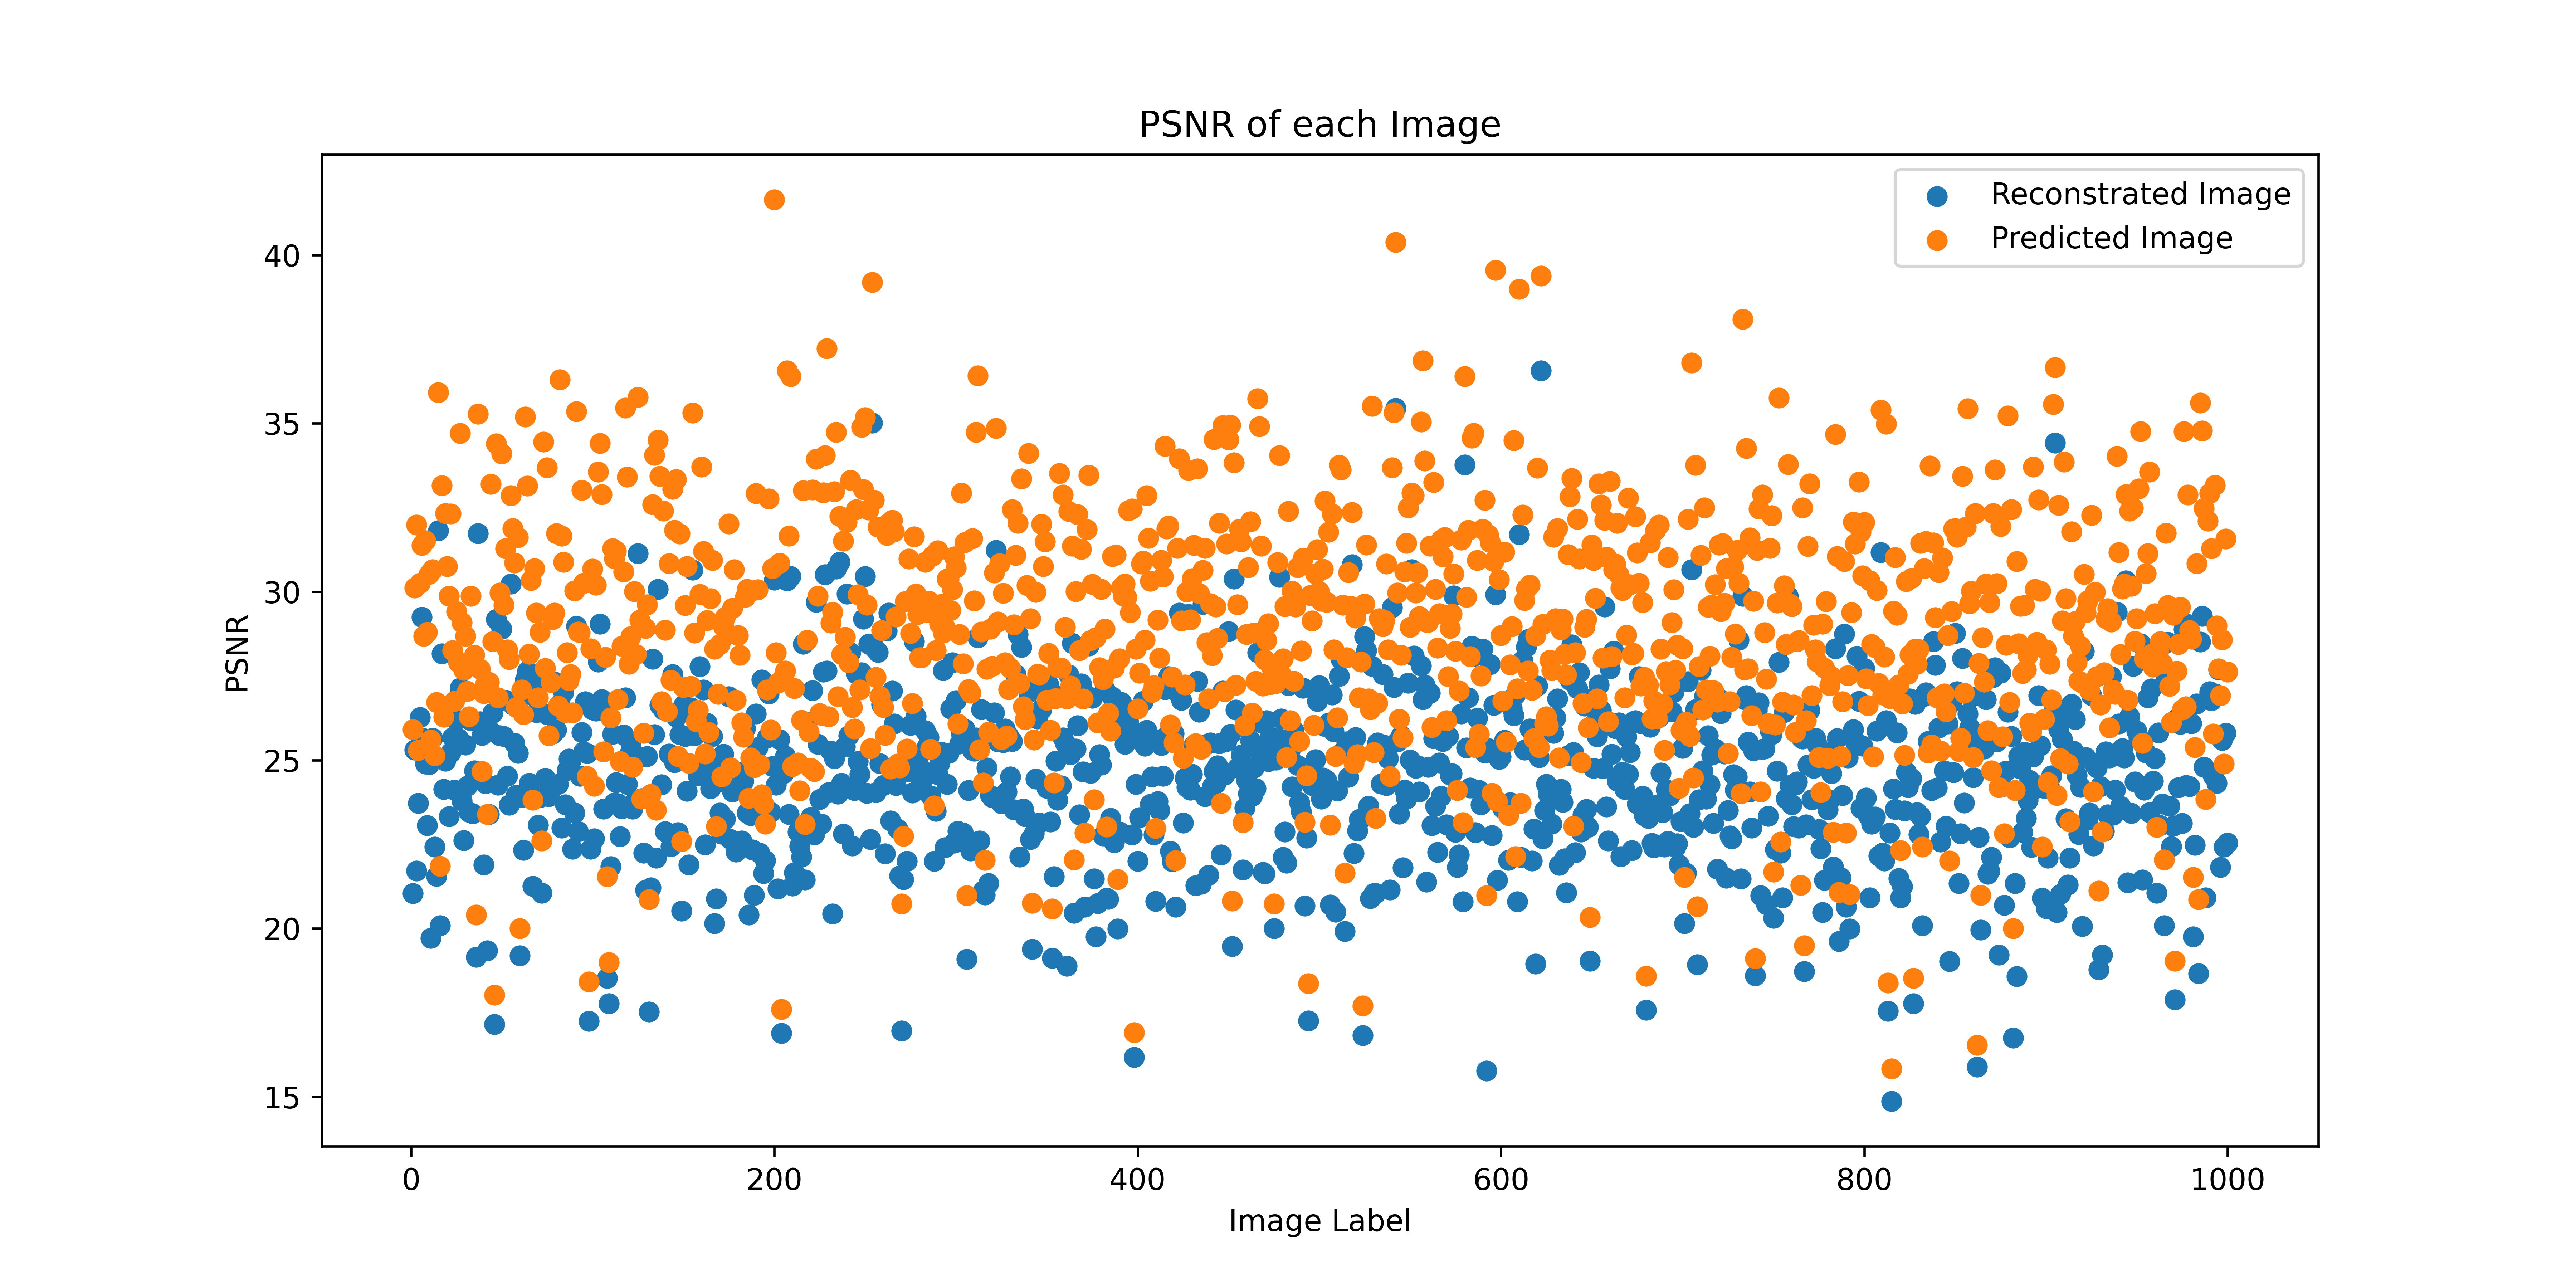
\includegraphics[width=0.9\columnwidth]{image/chap06/img603.png}
 	\caption{测试集图像及其预测图象与原图像的PSNR}
 	\label{fig603}
 \end{figure}

在图\ref{fig603}中,X轴为各图像的编号,Y轴为对应的PSNR值。从图\ref{fig603}可以看出,预测图象的PSNR值在图中的主要分布区域为上半区域,而重建图像的PSNR值主要分布在下半区域。计算这1000张重建图像与预测图像的PSNR值的平均值,计算结果如图\ref{fig604}。

\begin{figure}[h]
	\centering
	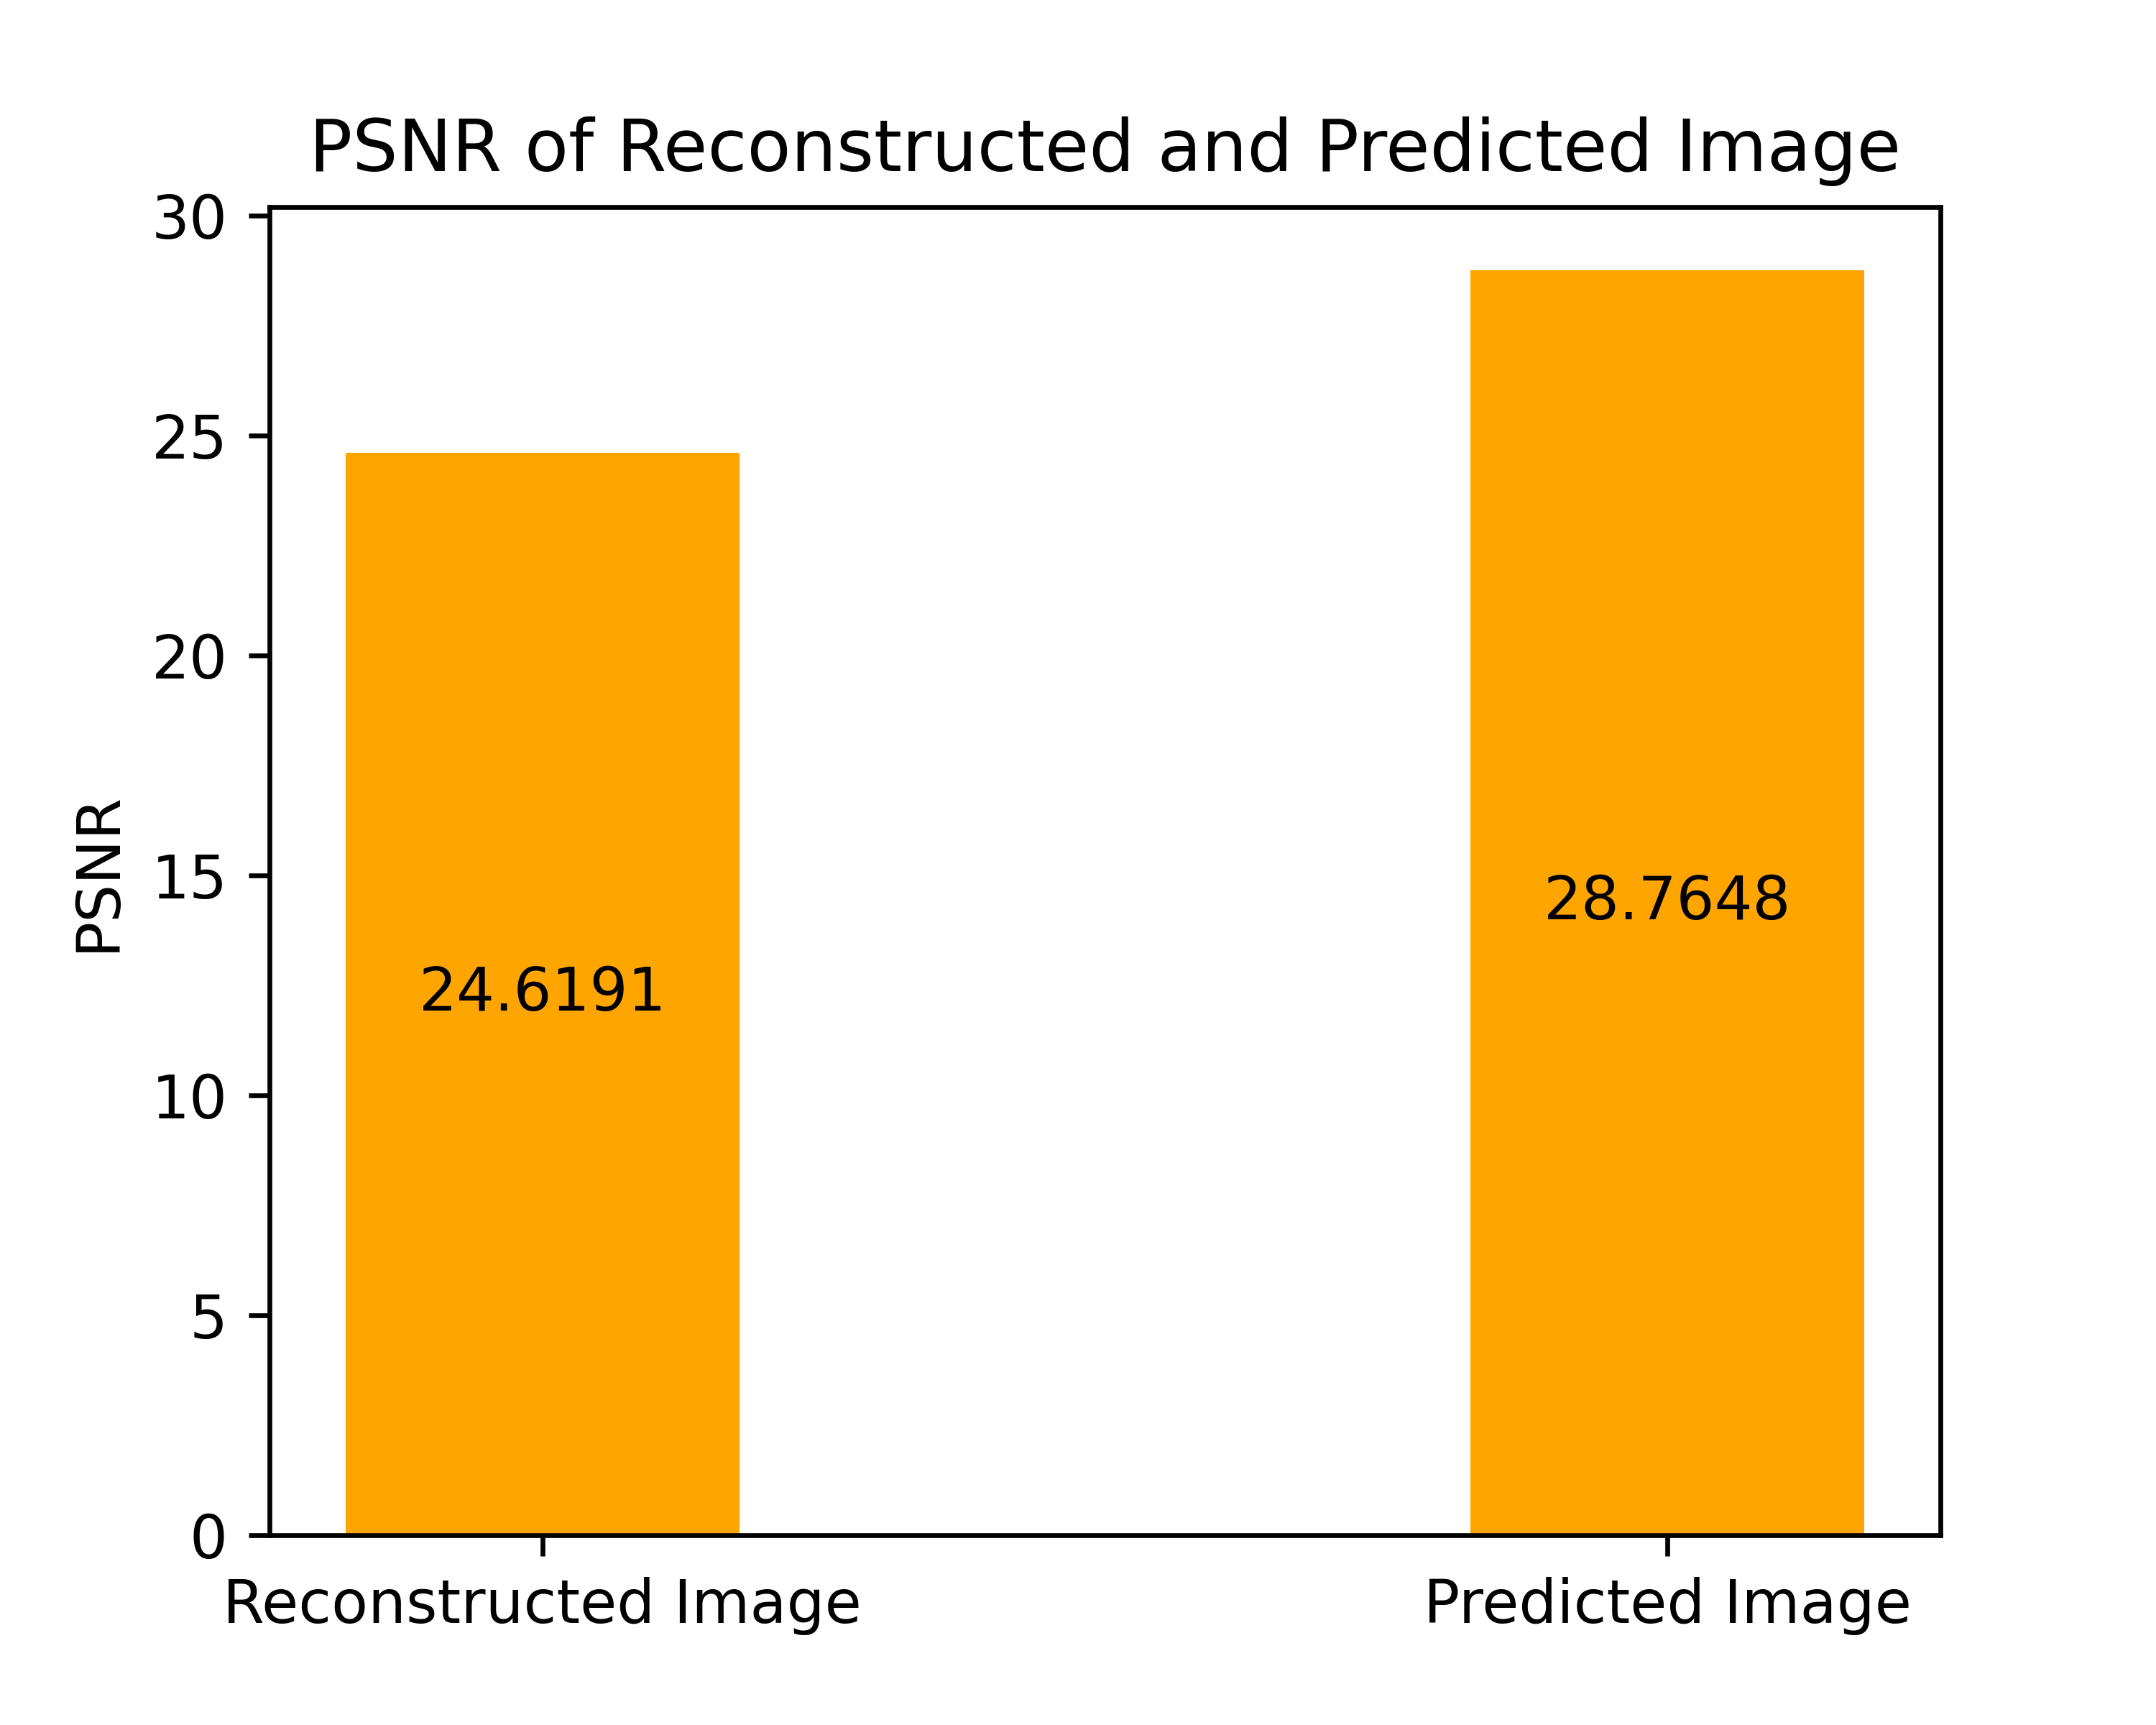
\includegraphics[width=0.75\columnwidth]{image/chap06/img604.png}
	\caption{测试集图像及其预测图象与原图像的PSNR的均值}
	\label{fig604}
\end{figure}

从图\ref{fig604}可以得出,在输入模型后所得优化图像,相比原来的重建图像,平均的PSNR值由24.6191上升为28.7638。由上述PSNR公式可得,更高的PSNR代表着更高的图像相似程度,这说明模型的预测图象相比于重建图像与原图像具有更高的相似度,模型具有良好的优化效果。

\section{SSIM}
\subsection{SSIM简介}
SSIM即结构相似度,它是一种判断两张图片在结构上的差距的一项指标。

与传统的 MSE 不同,对于两张图片基于 MSE 的损失大小不足以表达人类视觉系统对这两张图片所感觉到的差距。比如两张只是亮度不同的图片,由于MSE是计算二者像素差的平方之和,因此所计算出的损失很大,但在人眼看来,这两张图片是十分相近的。人类视觉相关的研究普遍认为人类衡量两幅图的差距,更倾向于比较两图的结构相似性,而不是像MSE那样逐像素计算两图的差异。

SSIM的衡量标准有两张图片的亮度相似度,对比度和结构相似度三个指标。

\subsubsection{亮度相似度}
设图像X所含的像素点个数为N,各像素值为$x_i$,则定义其平均亮度为X中各像素的均值,即:$\mu_X=\cfrac{1}{N}\sum_{i=1}^{N}x_i$

定义衡量两幅图 X 和 Y 的亮度相似度的公式为:

 \begin{equation} \label{603}
	l(X,Y)=\cfrac{2\mu_x\mu_y+C_1}{\mu_x^2+\mu_y^2+C_1}
\end{equation}

其中分母所在的常数是为了后续计算中避免出现分母为 0 的情况。

\subsubsection{对比度}
对比度定义为全体像素值的标准差,代表着图像明暗变化的剧烈程度。一张图像的标准差的计算公式为:
$\sigma_X=\sqrt{\cfrac{\sum_{i=1}^{N}(x_i-\mu_X)^2}{N-1}}$。
衡量两幅图 X 和 Y 的对比度的相似度的公式为:

 \begin{equation} \label{604}
	c(X,Y)=\cfrac{2\sigma_x\sigma_y+C_2}{\sigma_x^2+\sigma_y^2+C_2}
\end{equation}
同样地,分母中的常数是为了后续计算中避免出现分母为0的情况。

\subsubsection{结构相似度}
由于在上面的推导中已考虑亮度和对比度,因此在研究结构相似度时,应该首先排除这两个指标的影响,即将图像进行归一后以排除均值和标准差的影响。定义归一化后的两个向量 $\cfrac{X −\mu_X}{\sigma_X}$和 $\cfrac{Y −\mu_Y}{\sigma_Y}$之间的结构相似度为:

\begin{equation}\label{605}
	\begin{split}
		\ s(X,Y) &= \ \Big (\cfrac{1}{\sqrt{N-1}}\cfrac{X-\mu_X}{\sigma_X} \Big) \cdot \ \Big(\cfrac{1}{\sqrt{N-1}}\cfrac{Y-\mu_Y}{\sigma_Y}\Big)\\
		&= \cfrac{1}{\sigma_X\sigma_Y}\Big (\cfrac{1}{N-1}\sum_{i=1}^N(x_i-\mu_X)(y_i-\mu_Y) \Big )
	\end{split}
\end{equation}

上式中第一行“·”表示向量内积;第二行括号内的部分为协方差公式:$\sigma_{XY}=\cfrac{\sum_{i=1}^N(x_i-\mu_X)(y_i-\mu_Y)}{N-1}$。因此得到结构相似度的表达式为:

\begin{equation}\label{606}
s(X,Y)=\cfrac{\sigma_{XY}+C_3}{\sigma_X\sigma_Y+C_3}
\end{equation}
同理,为了防止后续计算出现分母为 0,分子分母同时加$C_3$。

\subsubsection{得出 SSIM 表达式}
由上面的推导得出的表达式(\ref{603})、(\ref{604})和(\ref{606}),三个标准相乘作为 SSIM 相似度公式,即:

\begin{equation}\label{607}
	SSIM(x,y)=l(x,y)^{\alpha}\cdot c(x,y)^{\beta} \cdot s(x,y)^{\gamma}
\end{equation}

公式中的$\alpha ,\beta ,\gamma$代表上述三个特征在SSIM指标中的占比,当三者都为1时,SSIM的表达式为:

\begin{equation}\label{608}
SSIM(X,Y)=\cfrac{(2\mu_X\mu_Y+C_1)(2\sigma_{XY}+C_2)}{(\mu_X^2+\mu_Y^2+C_1)(\sigma_X^2+\sigma_Y^2+C_2)}
\end{equation}

从以上的推导公式可知,两张图像的SSIM值是一个介于0和1之间的常数,且越接近1代表两张图像越是接近。从这个角度出发,接下来我们将尝试将SSIM作为指标来分析所得模型做出的预测图像的准确程度。

\subsection{使用SSIM衡量模型效果}
计算验证集中的1000张重建图像与原图像的SSIM值和预测图像与原图像的SSIM值,结果如图\ref{fig605}所示。

\begin{figure}[h]
	\centering
	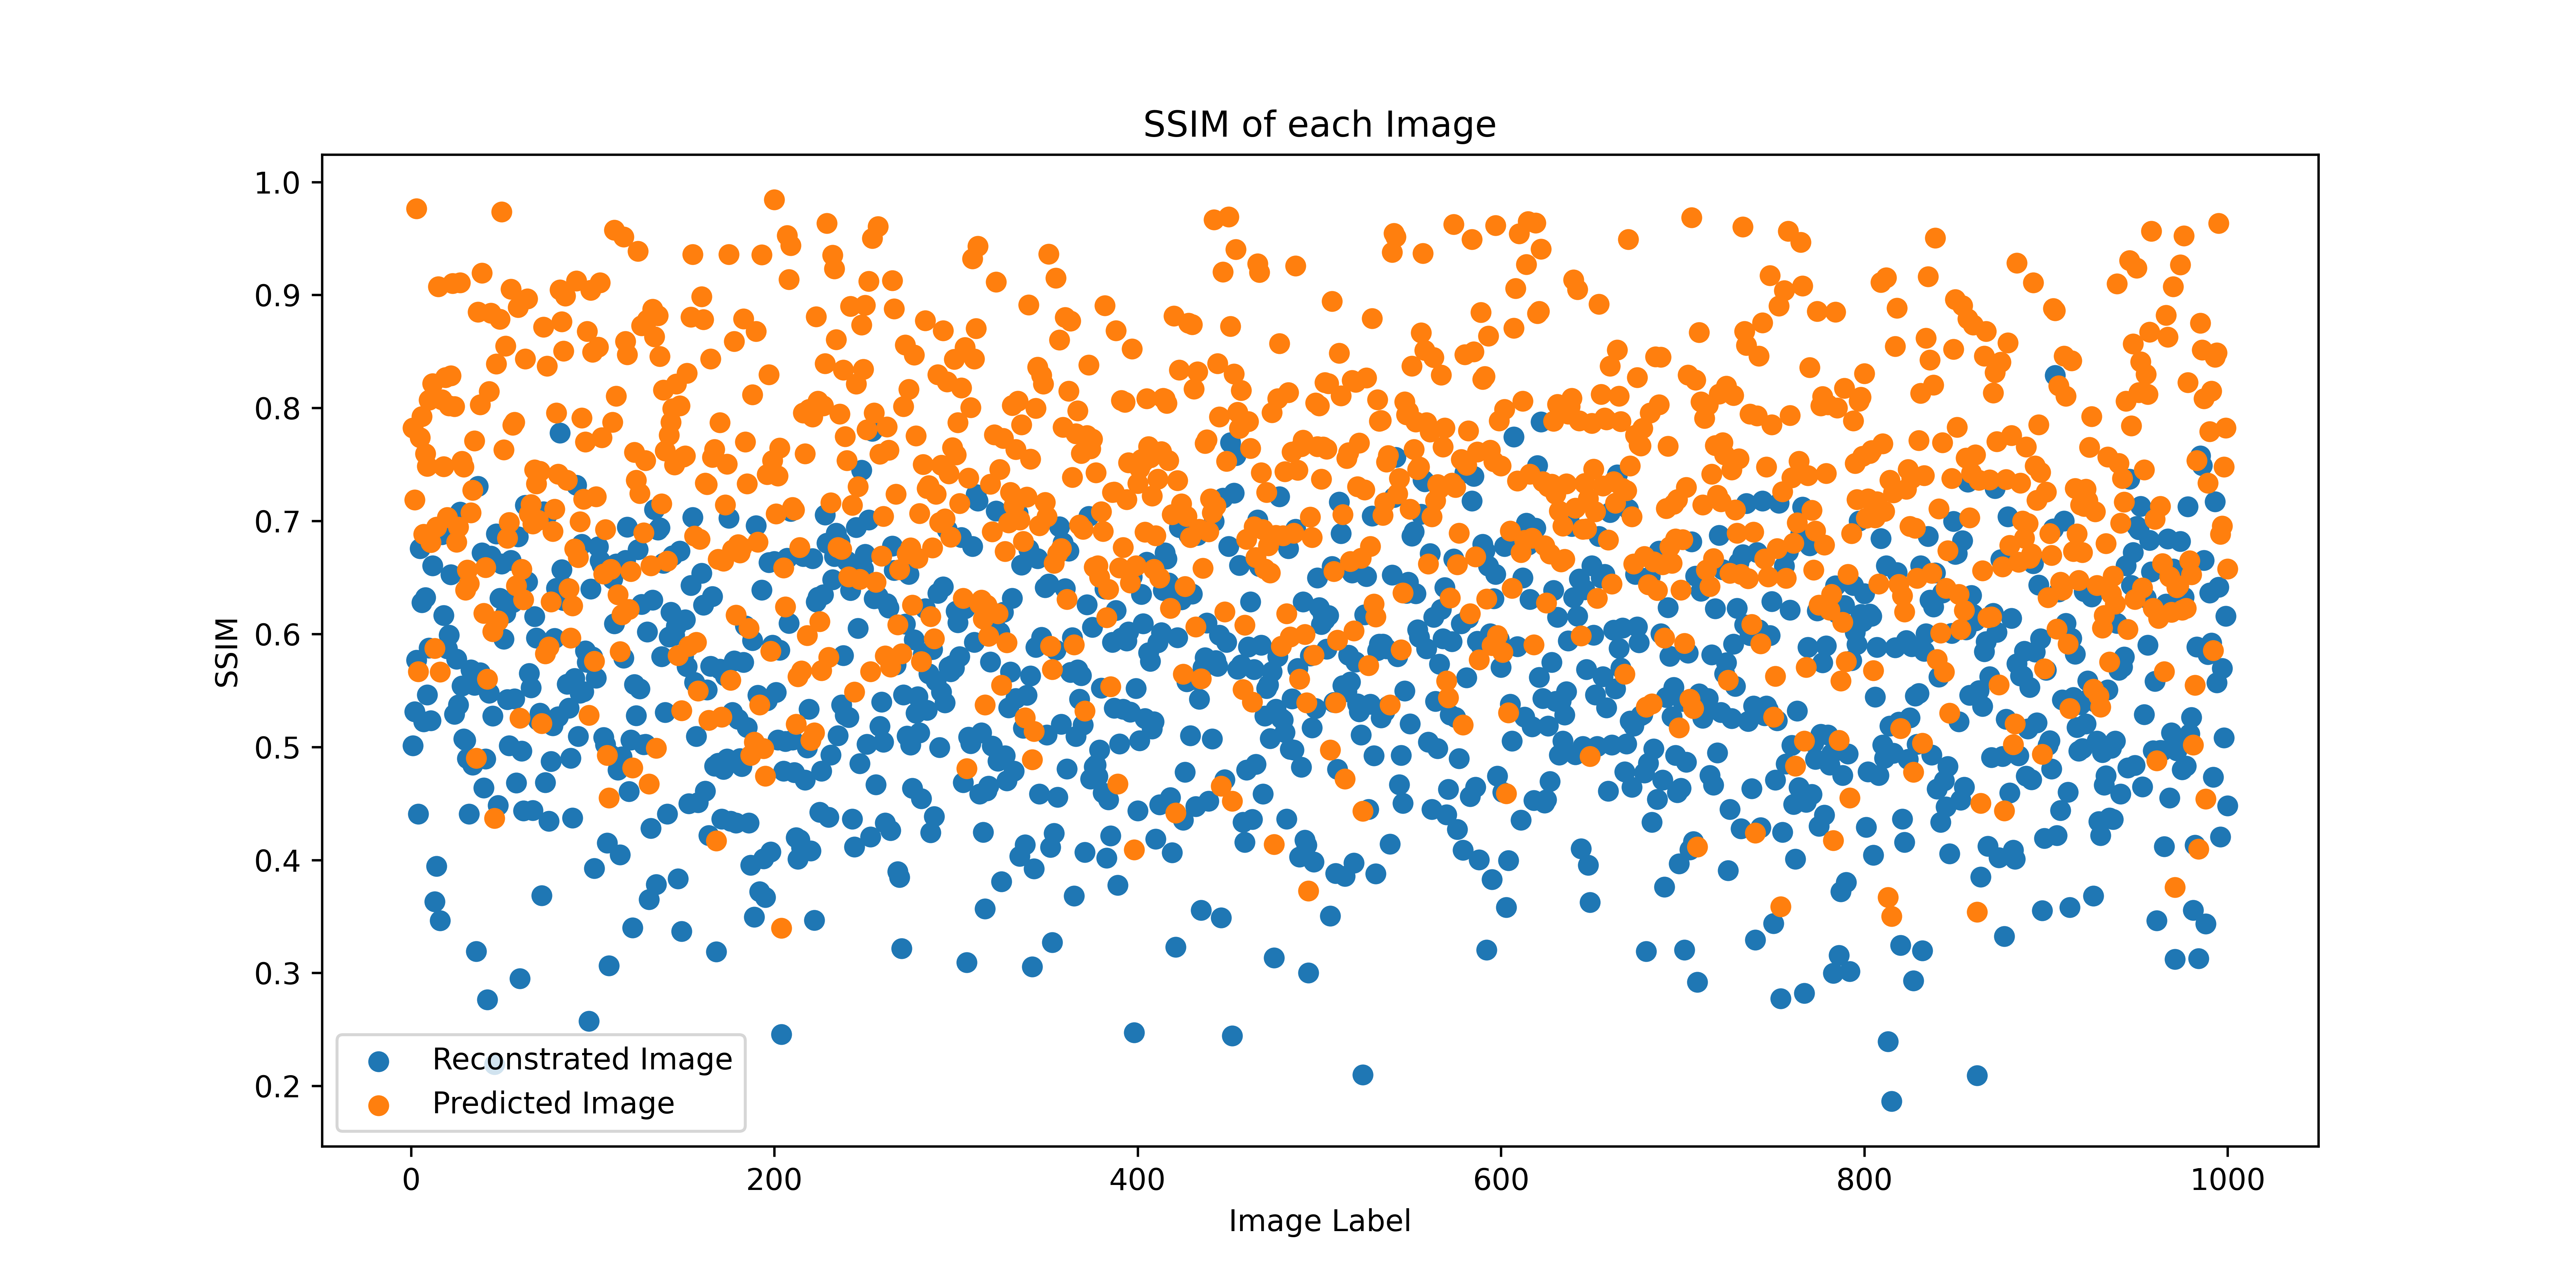
\includegraphics[width=0.9\columnwidth]{image/chap06/img605.png}
	\caption{测试集图像及其预测图象与原图像的SSIM}
	\label{fig605}
\end{figure}

在图\ref{fig605}中,X轴为各图像的编号,Y轴为SSIM值。从图\ref{fig605}可以看出,预测图象的SSIM值在图中大多分布在重建图像的SSIM值之上。而且计算这1000张重建图像与预测图像的SSIM值的平均值,计算结果如图\ref{fig606}。

\begin{figure}[h]
	\centering
	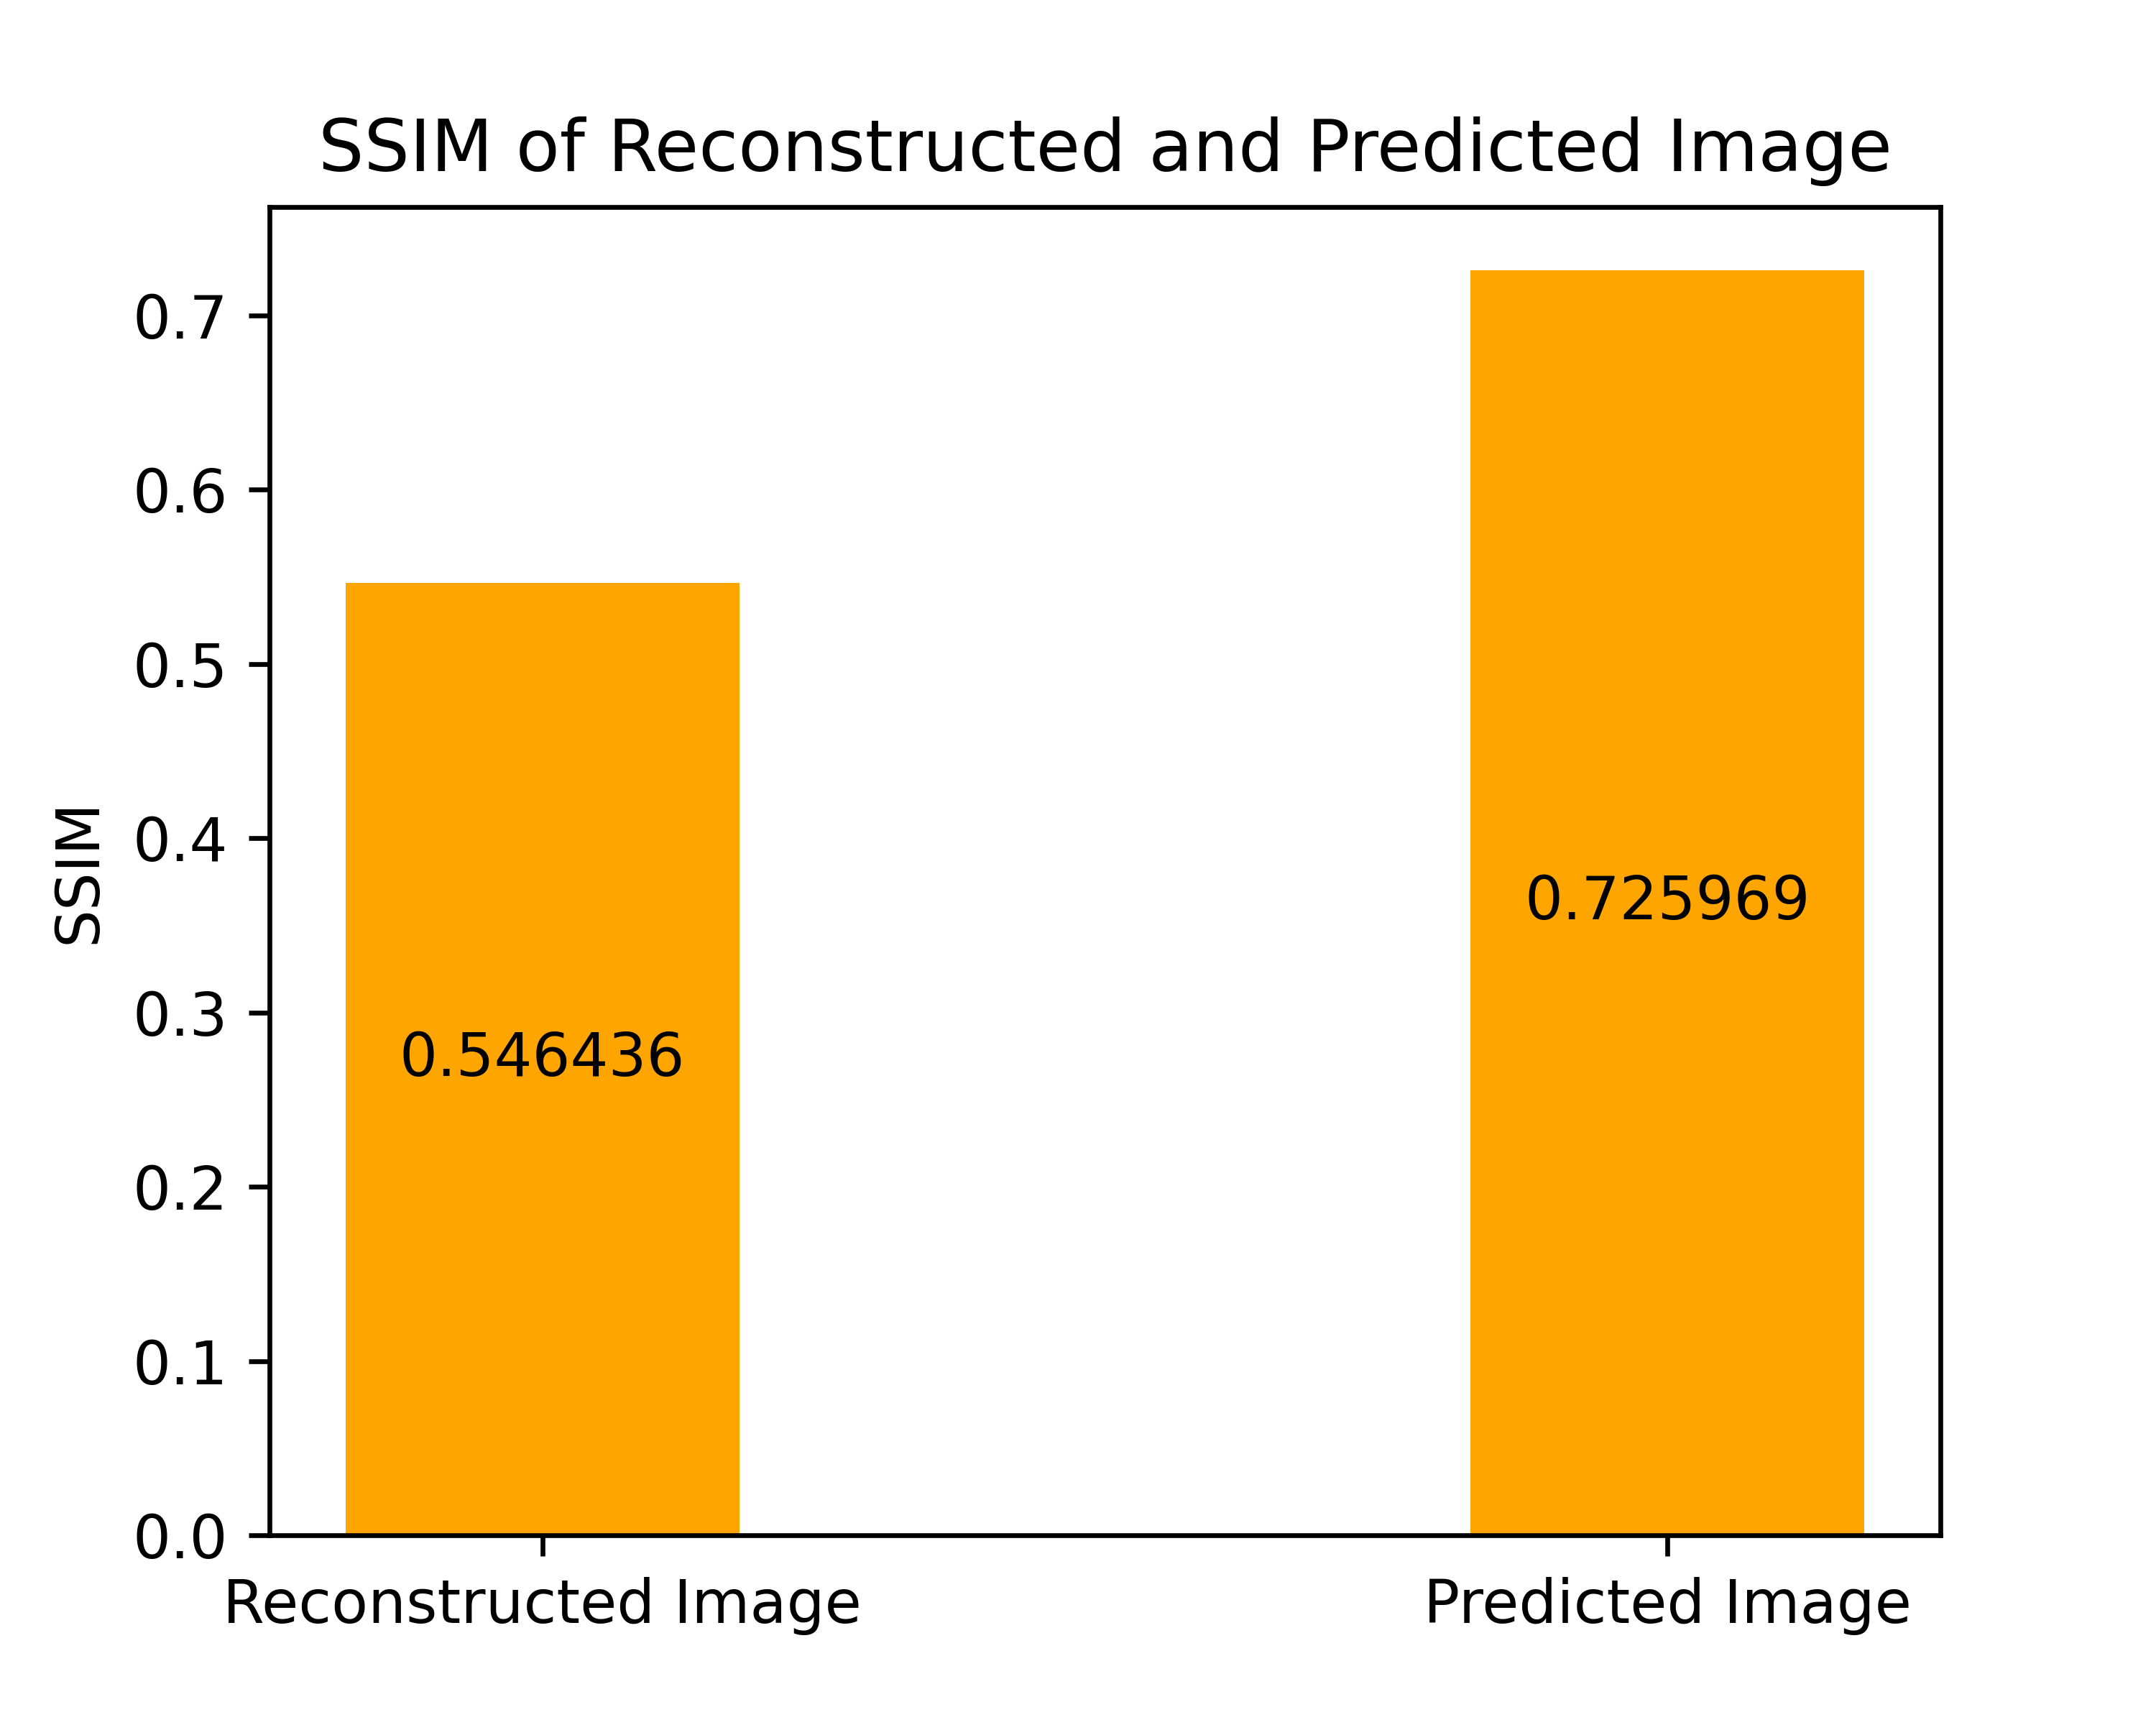
\includegraphics[width=0.75\columnwidth]{image/chap06/img606.png}
	\caption{测试集图像及其预测图象与原图像的SSIM的均值}
	\label{fig606}
\end{figure}

从图\ref{fig606}可以得出,在输入模型后所得优化图像,相比原来的重建图像,平均的SSIM值由0.55上升为0.73。可以发现预测图像对应的 SSIM 值比较接近 1,这说明从 SSIM 的角度上看,原图像与预测出的图像在亮度、对比度与结构相似度上较为接近,所以该模型的预测还是较为准确的。

\section{余弦相似度}
\subsection{余弦相似度简介}

余弦相似度是衡量两个向量相似程度的一项指标,即使用两个向量之间的夹角的余弦值作为衡量两者相似程度的标准。余弦值越接近于1,表示夹角越接近于0,表明两者越相似;反之,余弦值越接近于0,表示夹角约接近于$\cfrac{\pi}{2} $,表明两者越不相似。对于两个向量$X={x_i}$和$Y={y_i}$而言,其余弦相似度的计算公式为:

\begin{equation}\label{609}
	Cosine\ Similarity(X,Y)=\cfrac{\sum_{i=1}^n(x_i\times y_i)}{\sqrt{\sum_{i=1}^n(x_i)^2}\times \sqrt{\sum_{i=1}^n(y_i)^2}}
\end{equation}
我们可以将两张图片表示为向量后,使用余弦相似度来衡量两张图片的相似程度。

\subsection{使用余弦相似度衡量模型效果}
对验证集的1000张图像,我们计算了原图像与重建图像或预测图像间的余弦相似度,将其结果画成直方图如图\ref{fig607}所示。

\begin{figure}[h]
	\centering
	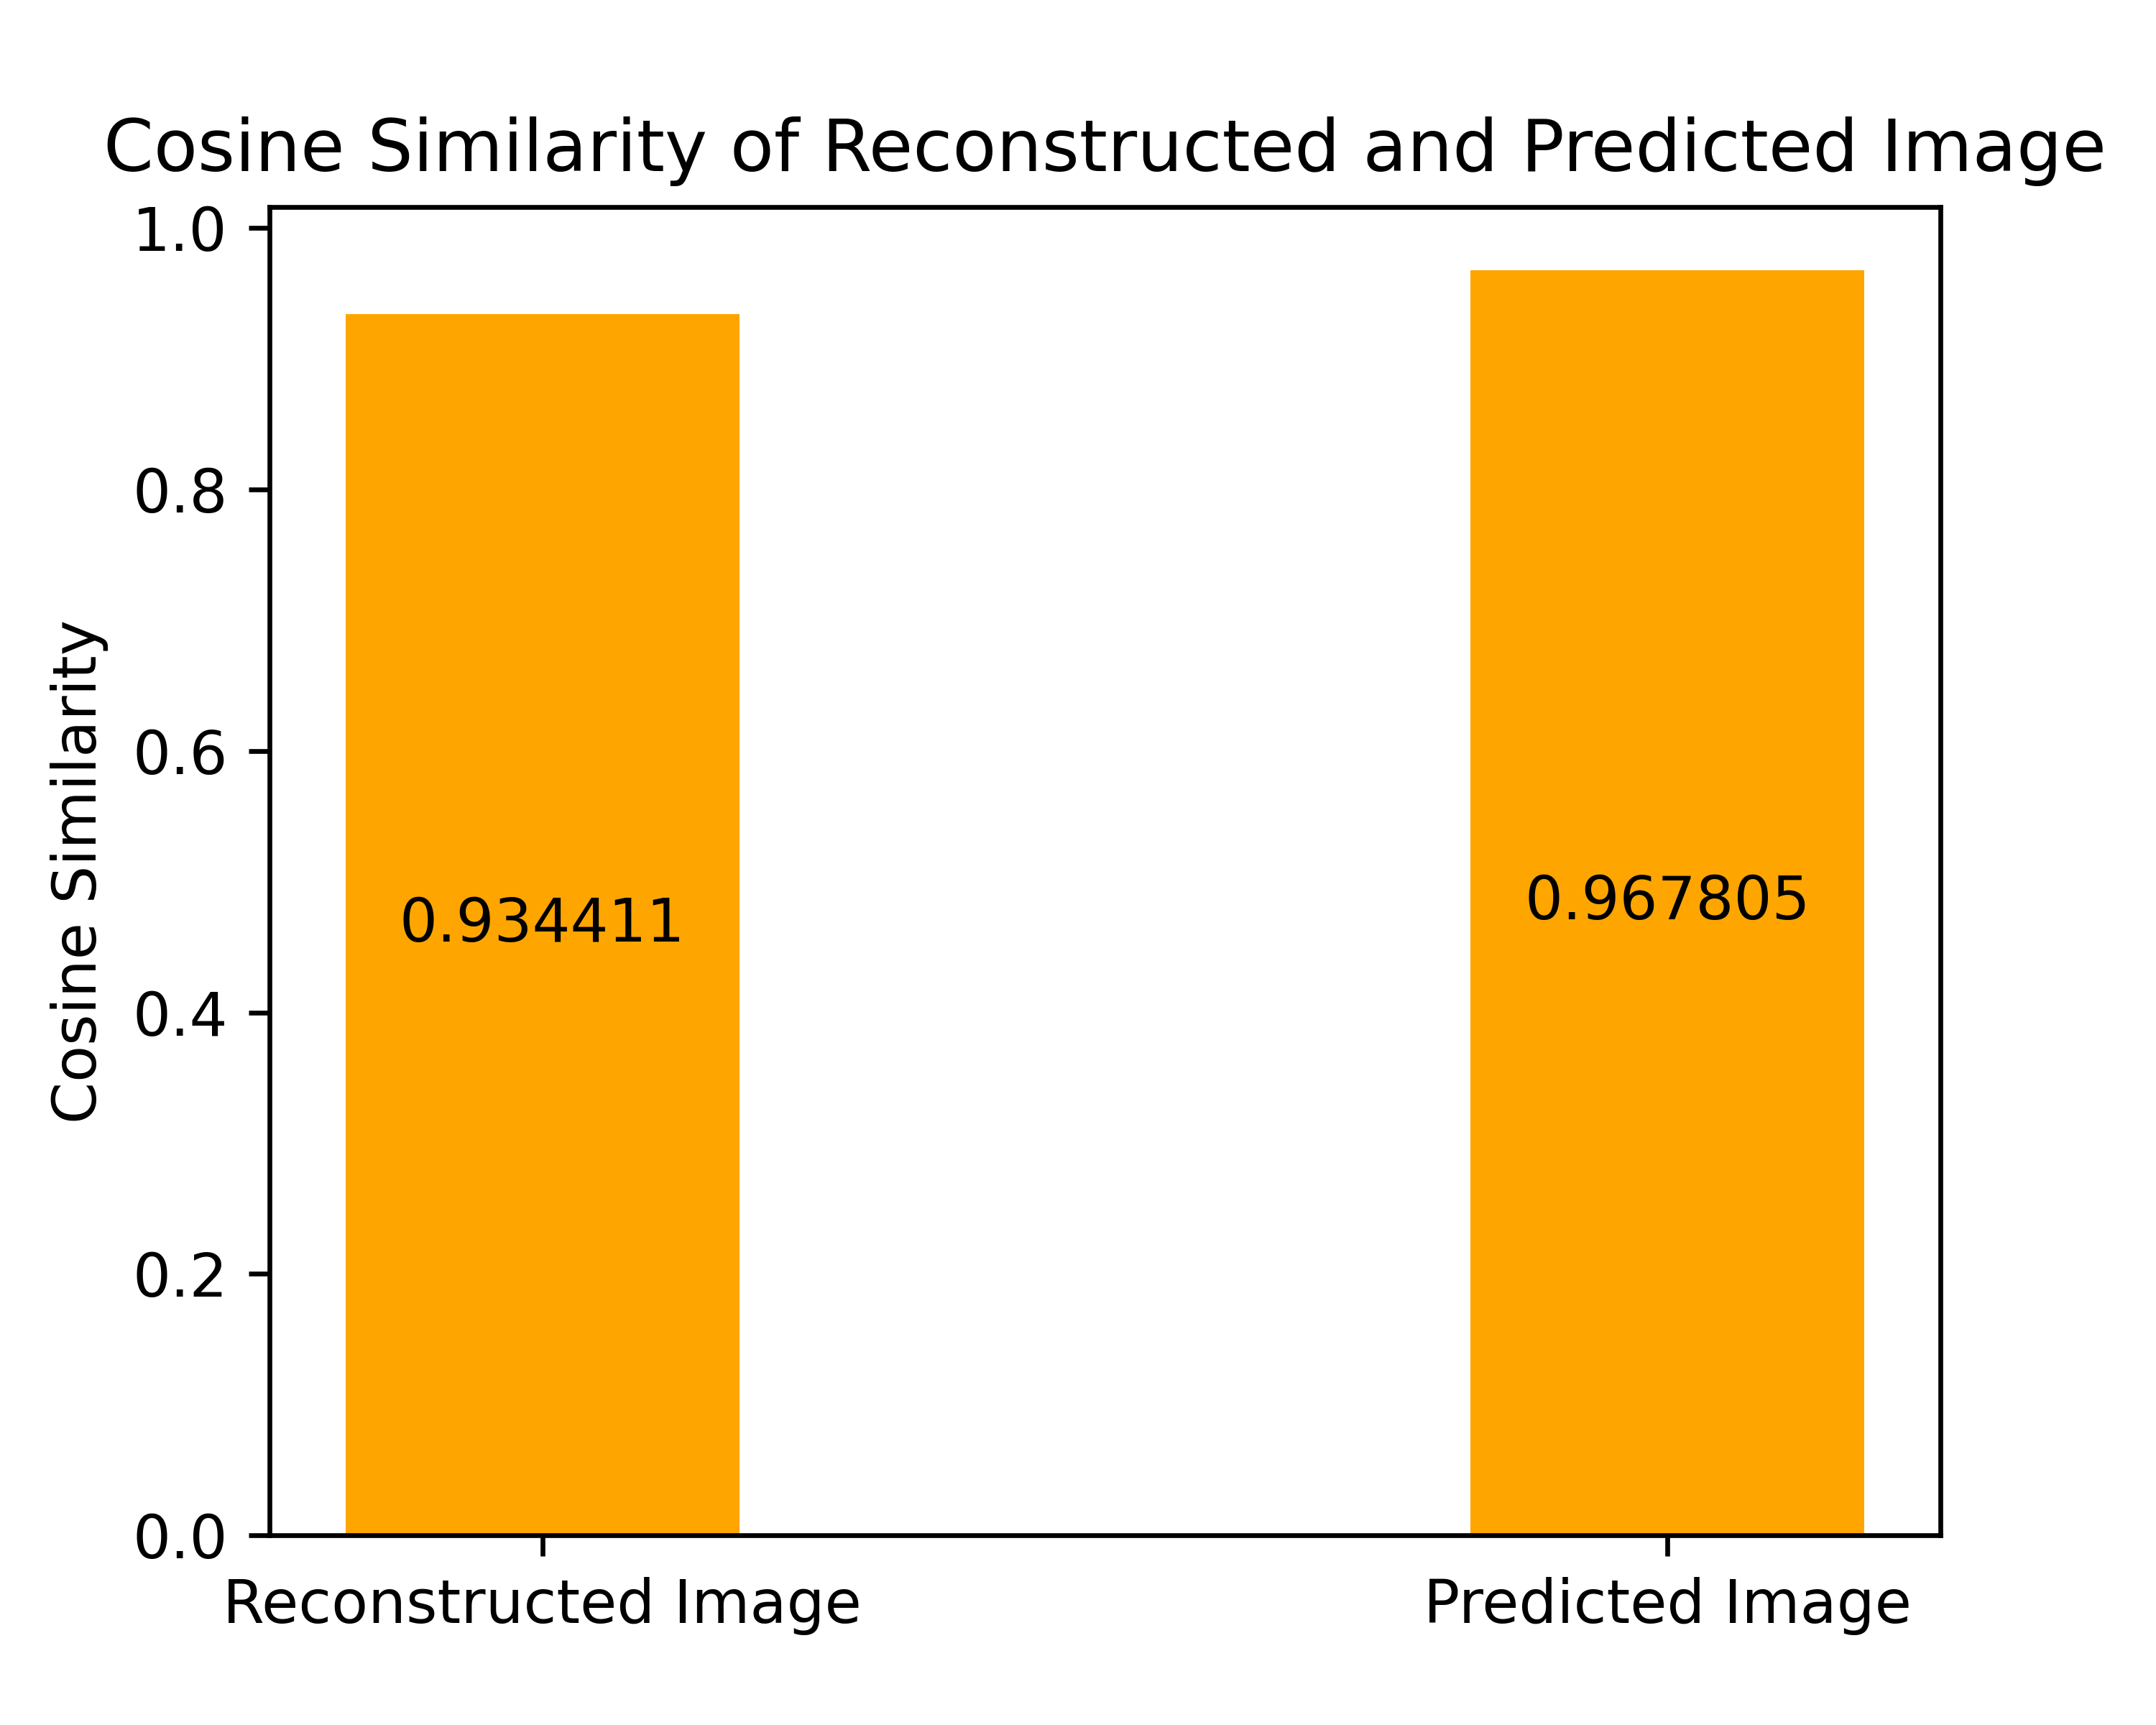
\includegraphics[width=0.75\columnwidth]{image/chap06/img607.png}
	\caption{测试集图像及其预测图象与原图像的余弦相似度的均值}
	\label{fig607}
\end{figure}

从上述结果可以看出,预测图像与原图像的余弦相似度大于重建图像与原图像间的余弦相似度,这说明在余弦相似度的指标下,预测图象对比重建图像具有更高的相似程度。

\section{哈希相似度}
\subsection{哈希相似度简介}
使用哈希值衡量两张图片的相似度分三步:第一步,计算两张图片各自的哈希值;第二步,计算两个哈希值之间的汉明距离(Hamming Distance);第三步,将汉明距离转化为两张图片的相似度。
\subsubsection{计算哈希值}
哈希值有三种定义方法,它们分别是均值哈希值(aHash),差值哈希值(dHash),感知哈希值(pHash)。它们的计算方法如下:
\begin{itemize}
	\item [1)]
	均值哈希值
	\begin{itemize}
		\item [$\bullet$]将图像缩放成如8x8像素大小的小图像并转为灰度图,计算小图像像素的均值。
		\item [$\bullet$]将小图像中比均值高的像素转换为1,比均值小的像素转换为0,生成哈希码。
	\end{itemize}
	
	\item [2)]
	差值哈希值
	\begin{itemize}
		\item [$\bullet$]将图像缩放成8x9像素大小的小图像并转为灰度图,使得每行9个像素之间存在8个不同的差异值。
		\item [$\bullet$]对于小图像中的相邻像素,若左像素比其右像素的值大,则左像素转换为1;否则转换为0,最终得到一个8x8的哈希矩阵。
	\end{itemize}

	\item [3)]
	感知哈希值
	\begin{itemize}
		\item [$\bullet$]将图像缩放成如8x8像素大小的小图像并转为灰度图
		\item [$\bullet$]对小图像进行32x32的DCT(离散余弦变换)得到32x32的DCT系数矩阵,并取左上角的8x8的矩阵,计算该矩阵的平均值。
		\item [$\bullet$]将8x8矩阵中比均值高的元素转换为1,比均值小的元素转换为0,生成哈希码。
	\end{itemize}
	
\end{itemize}

\subsubsection{计算汉明距离}
汉明距离即两个哈希值之间不相等的元素个数。

\subsubsection{将汉明距离转化为两张图片的相似度}
转化为相似度的公式为:

\begin{equation}\label{610}
similarity = 1 - \cfrac{dist}{pixelnum}
\end{equation}
其中dist为汉明距离,pixelnum为小图像的像素个数(若小图像为8x8,则pixelnum等于64)

\subsection{使用哈希相似度衡量模型效果}
对验证集的1000张图像,我们计算了原图像与重建图像或预测图像间的三种哈希相似度,将其结果画成直方图如图\ref{fig608}所示。

\begin{figure}[h]
	\centering
	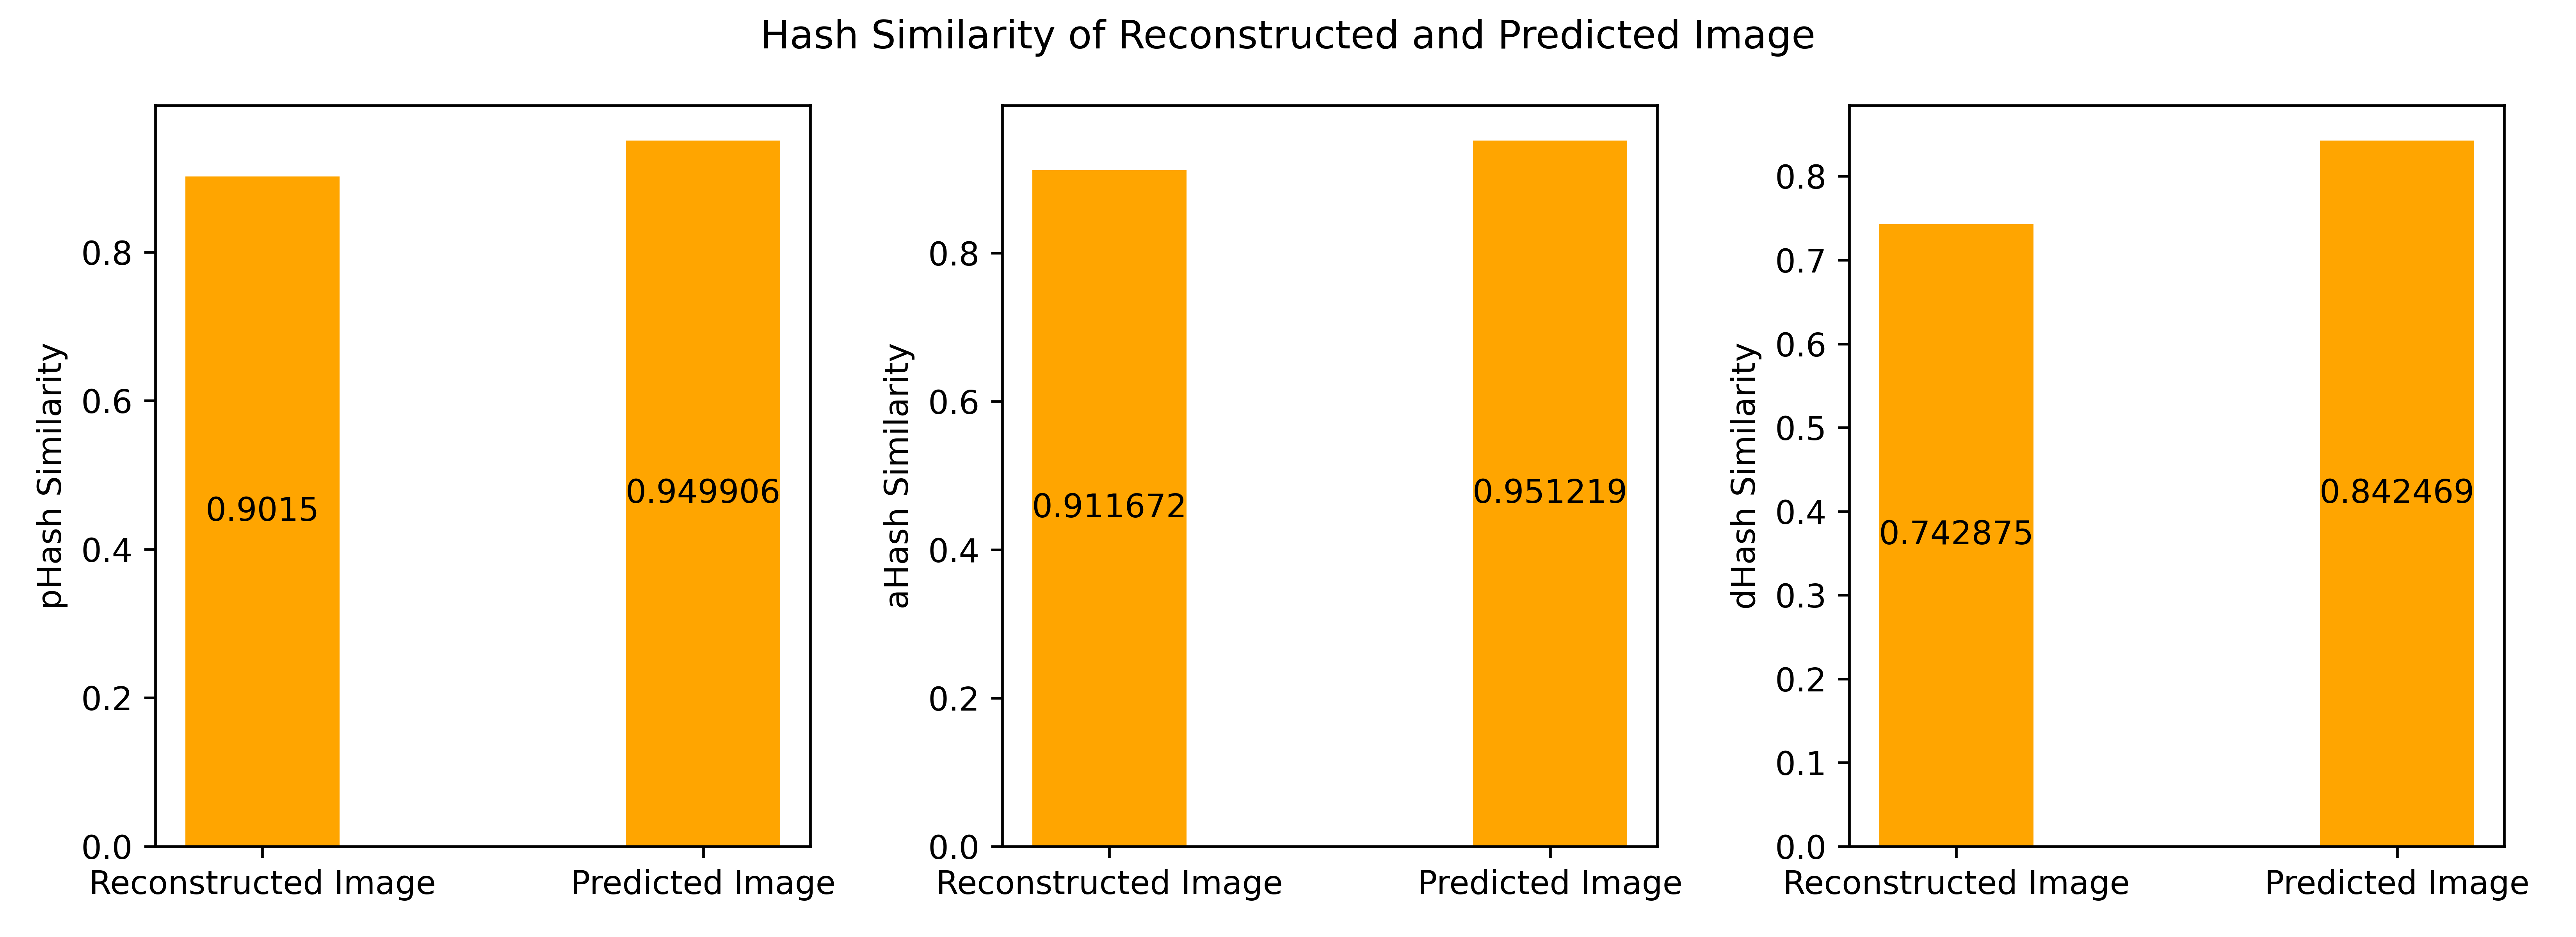
\includegraphics[width=0.9\columnwidth]{image/chap06/img608.png}
	\caption{测试集图像及其预测图象与原图像的三种哈希相似度的均值}
	\label{fig608}
\end{figure}

从图\ref{fig608}可得,无论是均值哈希值,差值哈希值还是感知哈希值,预测图像的相似度均大于重建图像的相似度。

\section{直方图相似度}
\subsection{直方图简介}
图像的直方图即统计全图各像素值所占的像素个数的直方图。对于256值的灰度图而言,就是统计0$ \sim $255这256个值的像素个数所作而成的直方图。例如皮肤癌数据集图像的直方图见图\ref{fig609}。

\begin{figure}[h]
	\centering
	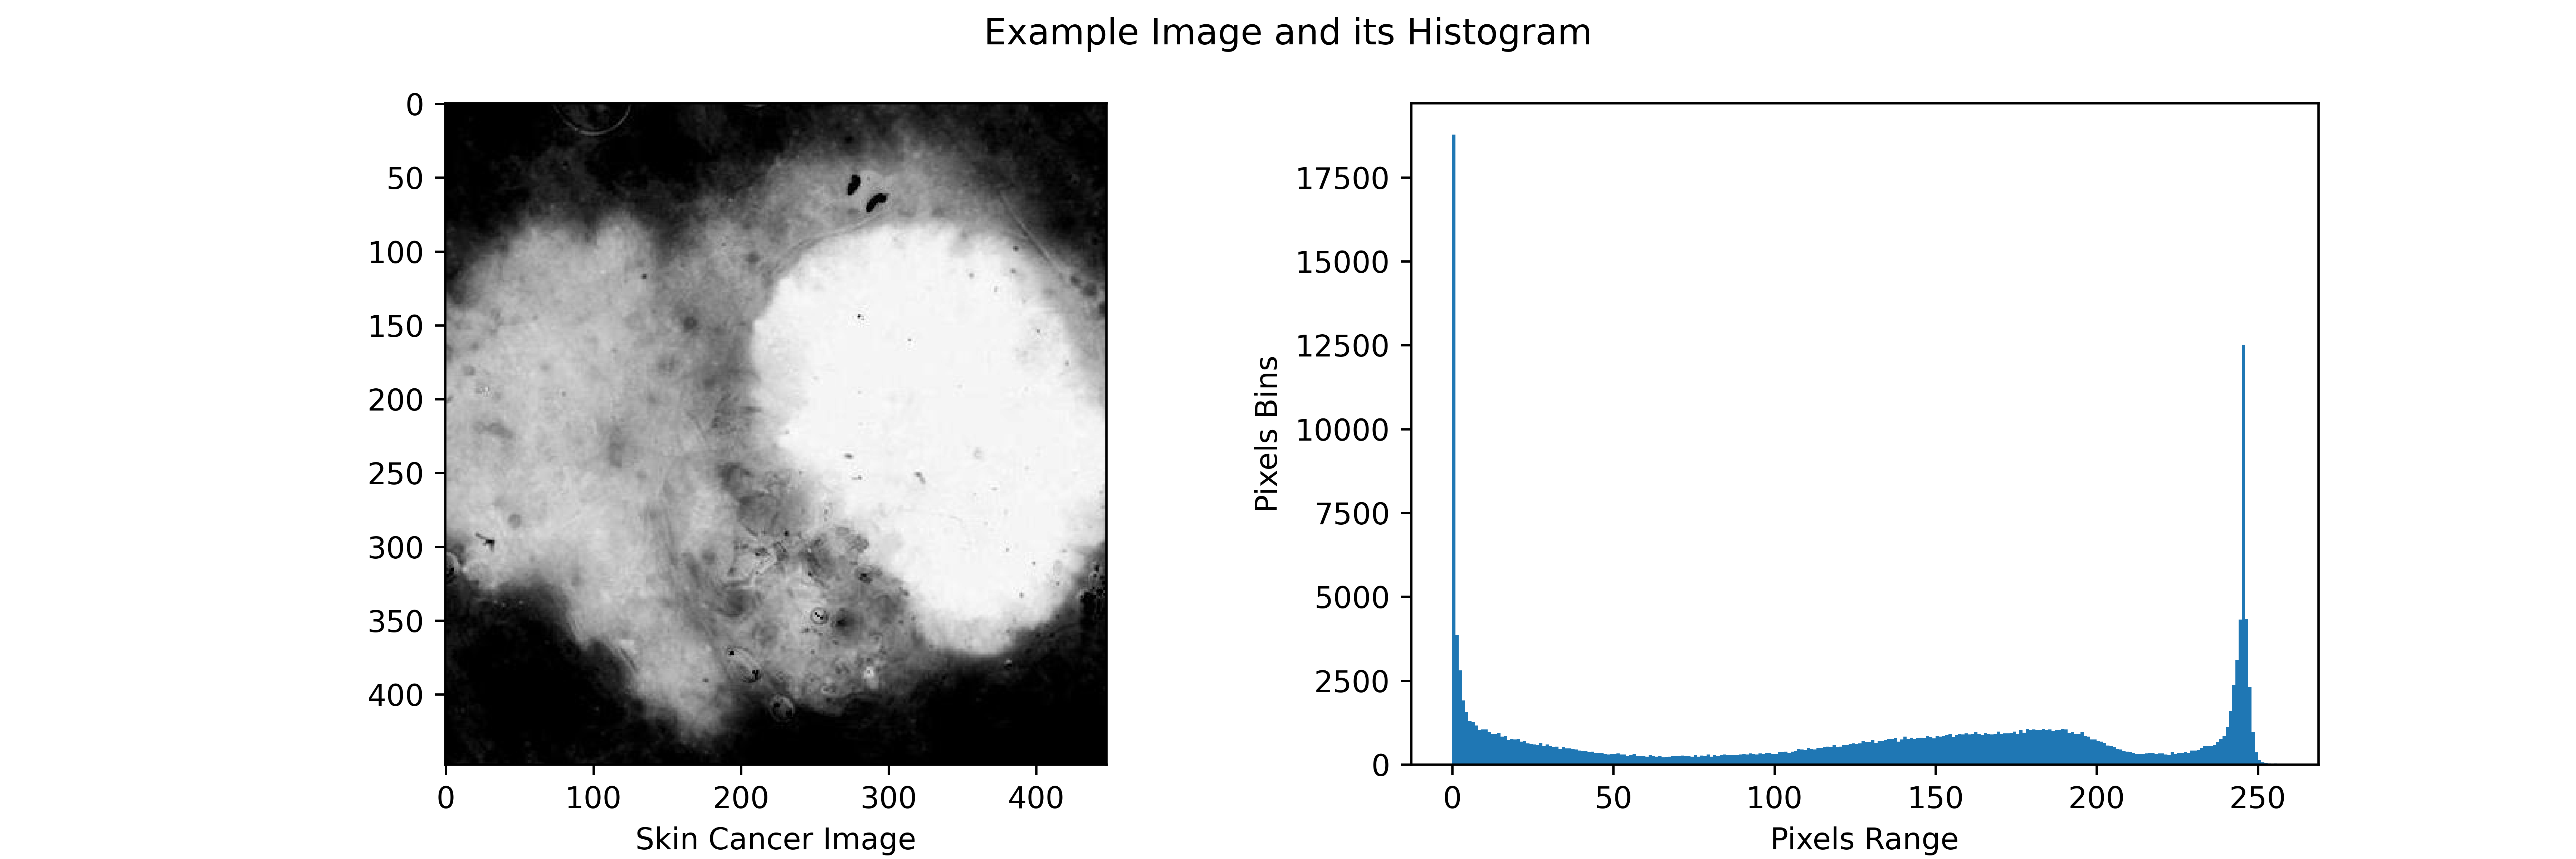
\includegraphics[width=0.9\columnwidth]{image/chap06/img609.png}
	\caption{皮肤癌图片的直方图}
	\label{fig609}
\end{figure}

\hspace*{\fill} \

\hspace*{\fill} \

\hspace*{\fill} \

\hspace*{\fill} \

假设$hist_1$和$hist_2$是存放着0$ \sim $255像素值所占像素个数的数组,则两个图像间的直方图相似度的计算公式为:

\begin{equation}\label{609}
	Degree(hist_1,hist_2)=\sum_i\cfrac{1 - |hist_1[i] - hist_2[i]|}{max(hist_1[i],hist_2[i])}
\end{equation}

\subsection{使用直方图相似度衡量模型效果}
对验证集的1000张图像,我们计算了原图像与重建图像或预测图像间的直方图相似度,其结果如图\ref{fig610}所示。

\begin{figure}[h]
	\centering
	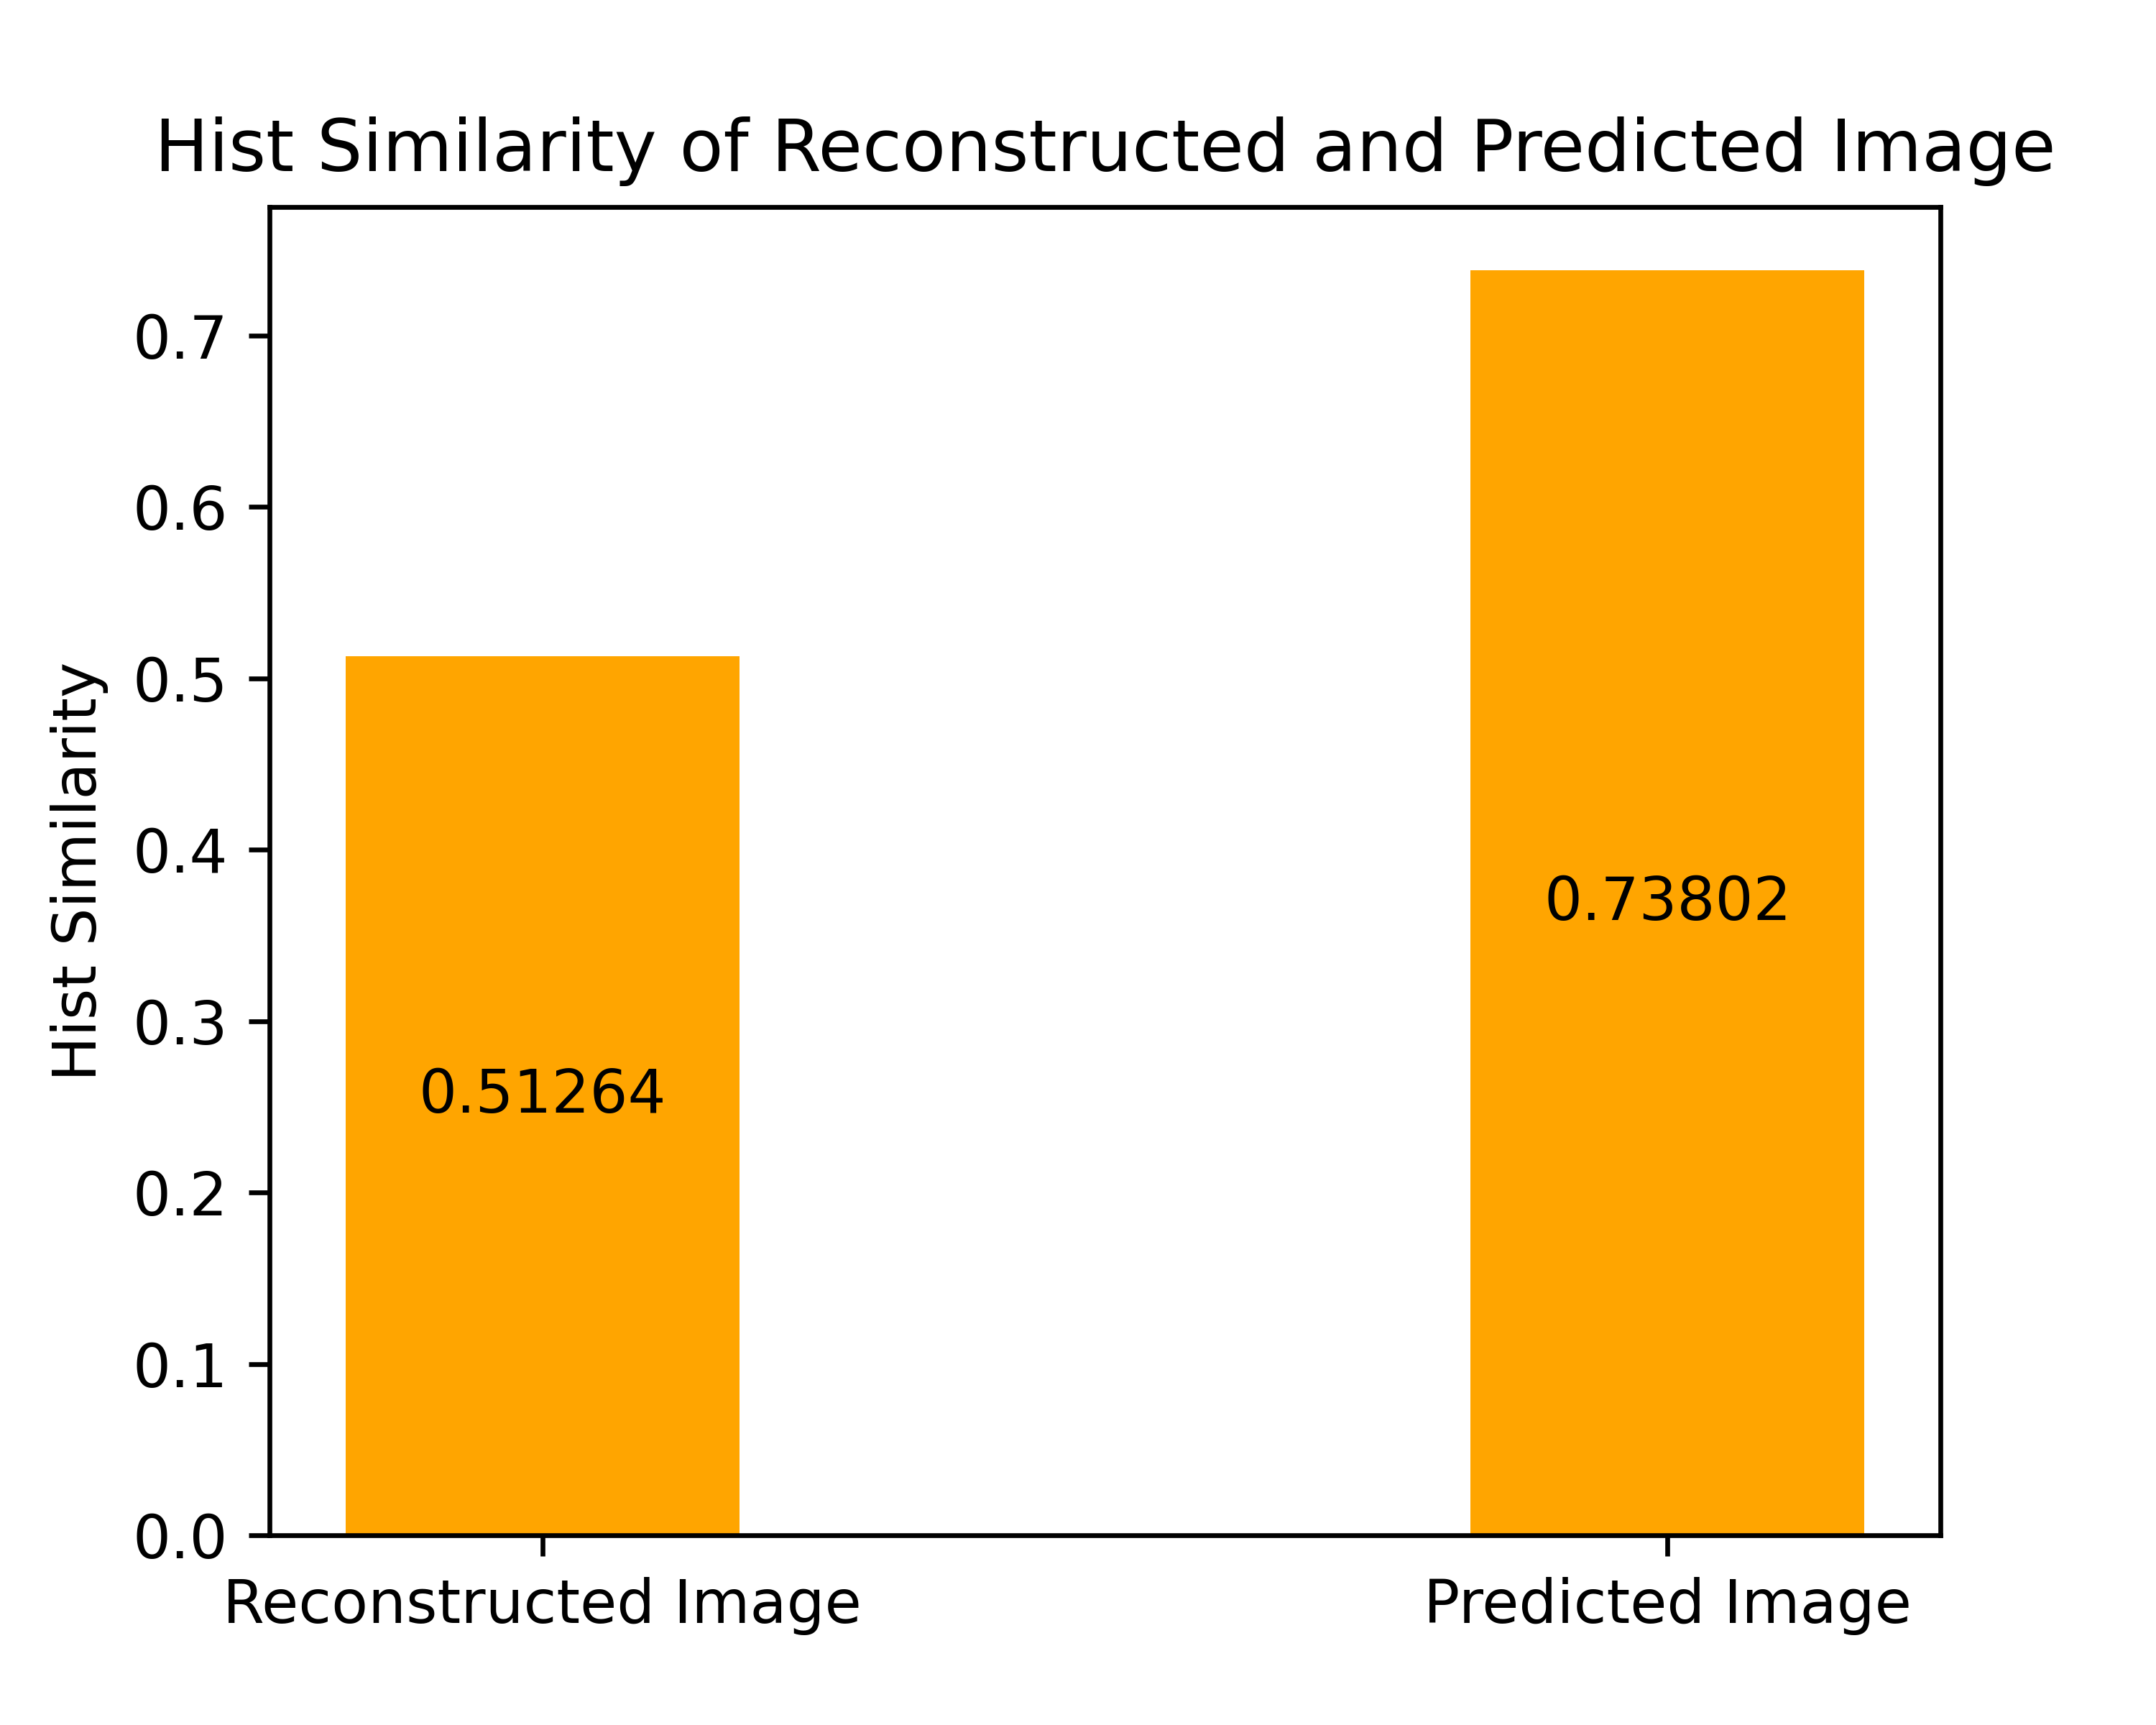
\includegraphics[width=0.75\columnwidth]{image/chap06/img610.png}
	\caption{测试集图像及其预测图象与原图像的直方图相似度的均值}
	\label{fig610}
\end{figure}

由图\ref{fig610}可知,重建图像与原图像之间的直方图相似度低于预测图像与原图像之间的直方图相似度。这说明预测图像相比于重建图像,在各像素值的统计学标准上更接近于原图像。

\section{归一化互信息}
\subsection{归一化互信息简介}
在信息论中,归一化互信息(NMI)是衡量两个随机变量之间的依赖程度大小的一项指标。NMI的值越大代表两个随机变量间的依赖程度越高。若将其运用于分析两个图片间的相似程度,则NMI的值越大代表两张图片具有越高的相似性。

对于两幅图像A与B,其归一化互信息的计算分成三步:

\begin{enumerate}
	\item 分别计算图像A,B的信息熵,其计算公式如下。
	
	\begin{equation}\label{612}
		H(A) = -\sum_aP_A(a)log_2P_A(a)
	\end{equation}

	\begin{equation}\label{613}
		H(B) = -\sum_bP_B(b)log_2P_B(b)
	\end{equation}

	其中,公式中a为图像A中的各像素值(若A为256值的灰度图像,则a的取值范围为[0,255])。像素值a的概率值$P_A(a)$为对图像进行灰度直方图统计后,像素值a所占像素点个数占全图像素点个数的比例值。对于公式(\ref{613})同理。
	
	\item 使用A与B各自的信息熵计算二者的联合信息熵。
	
	\begin{equation}\label{614}
		H(A,B)=-\sum_{a,b}P_{AB}(a,b)log_2P_{AB}(a,b)
	\end{equation}
	
	其中,公式中的a,b为图像A、B的各像素值(若A、B为256值的灰度图像,则a、b的取值范围均为[0,255]);联合概率密度$P_{AB}(a,b)$指的是两图在相同坐标系下,满足A的像素值为a且B的像素值为b的像素点,其个数占全图总像素点个数的比例值。
	
	\item 计算归一化信息熵。将第一第二步计算的A与B的信息熵H(A),H(B)及其联合信息熵H(A,B)代入如下的公式中得到归一化信息熵。
	
	\begin{equation}\label{615}
		NMI(A,B)=\cfrac{H(A)+H(B)}{H(A,B)}
	\end{equation}
\end{enumerate}

\subsection{使用互信息衡量模型效果}
对验证集的1000张图像,我们计算了原图像与重建图像或预测图像间的归一化互信息,其结果如图\ref{fig611}所示。

\begin{figure}[h]
	\centering
	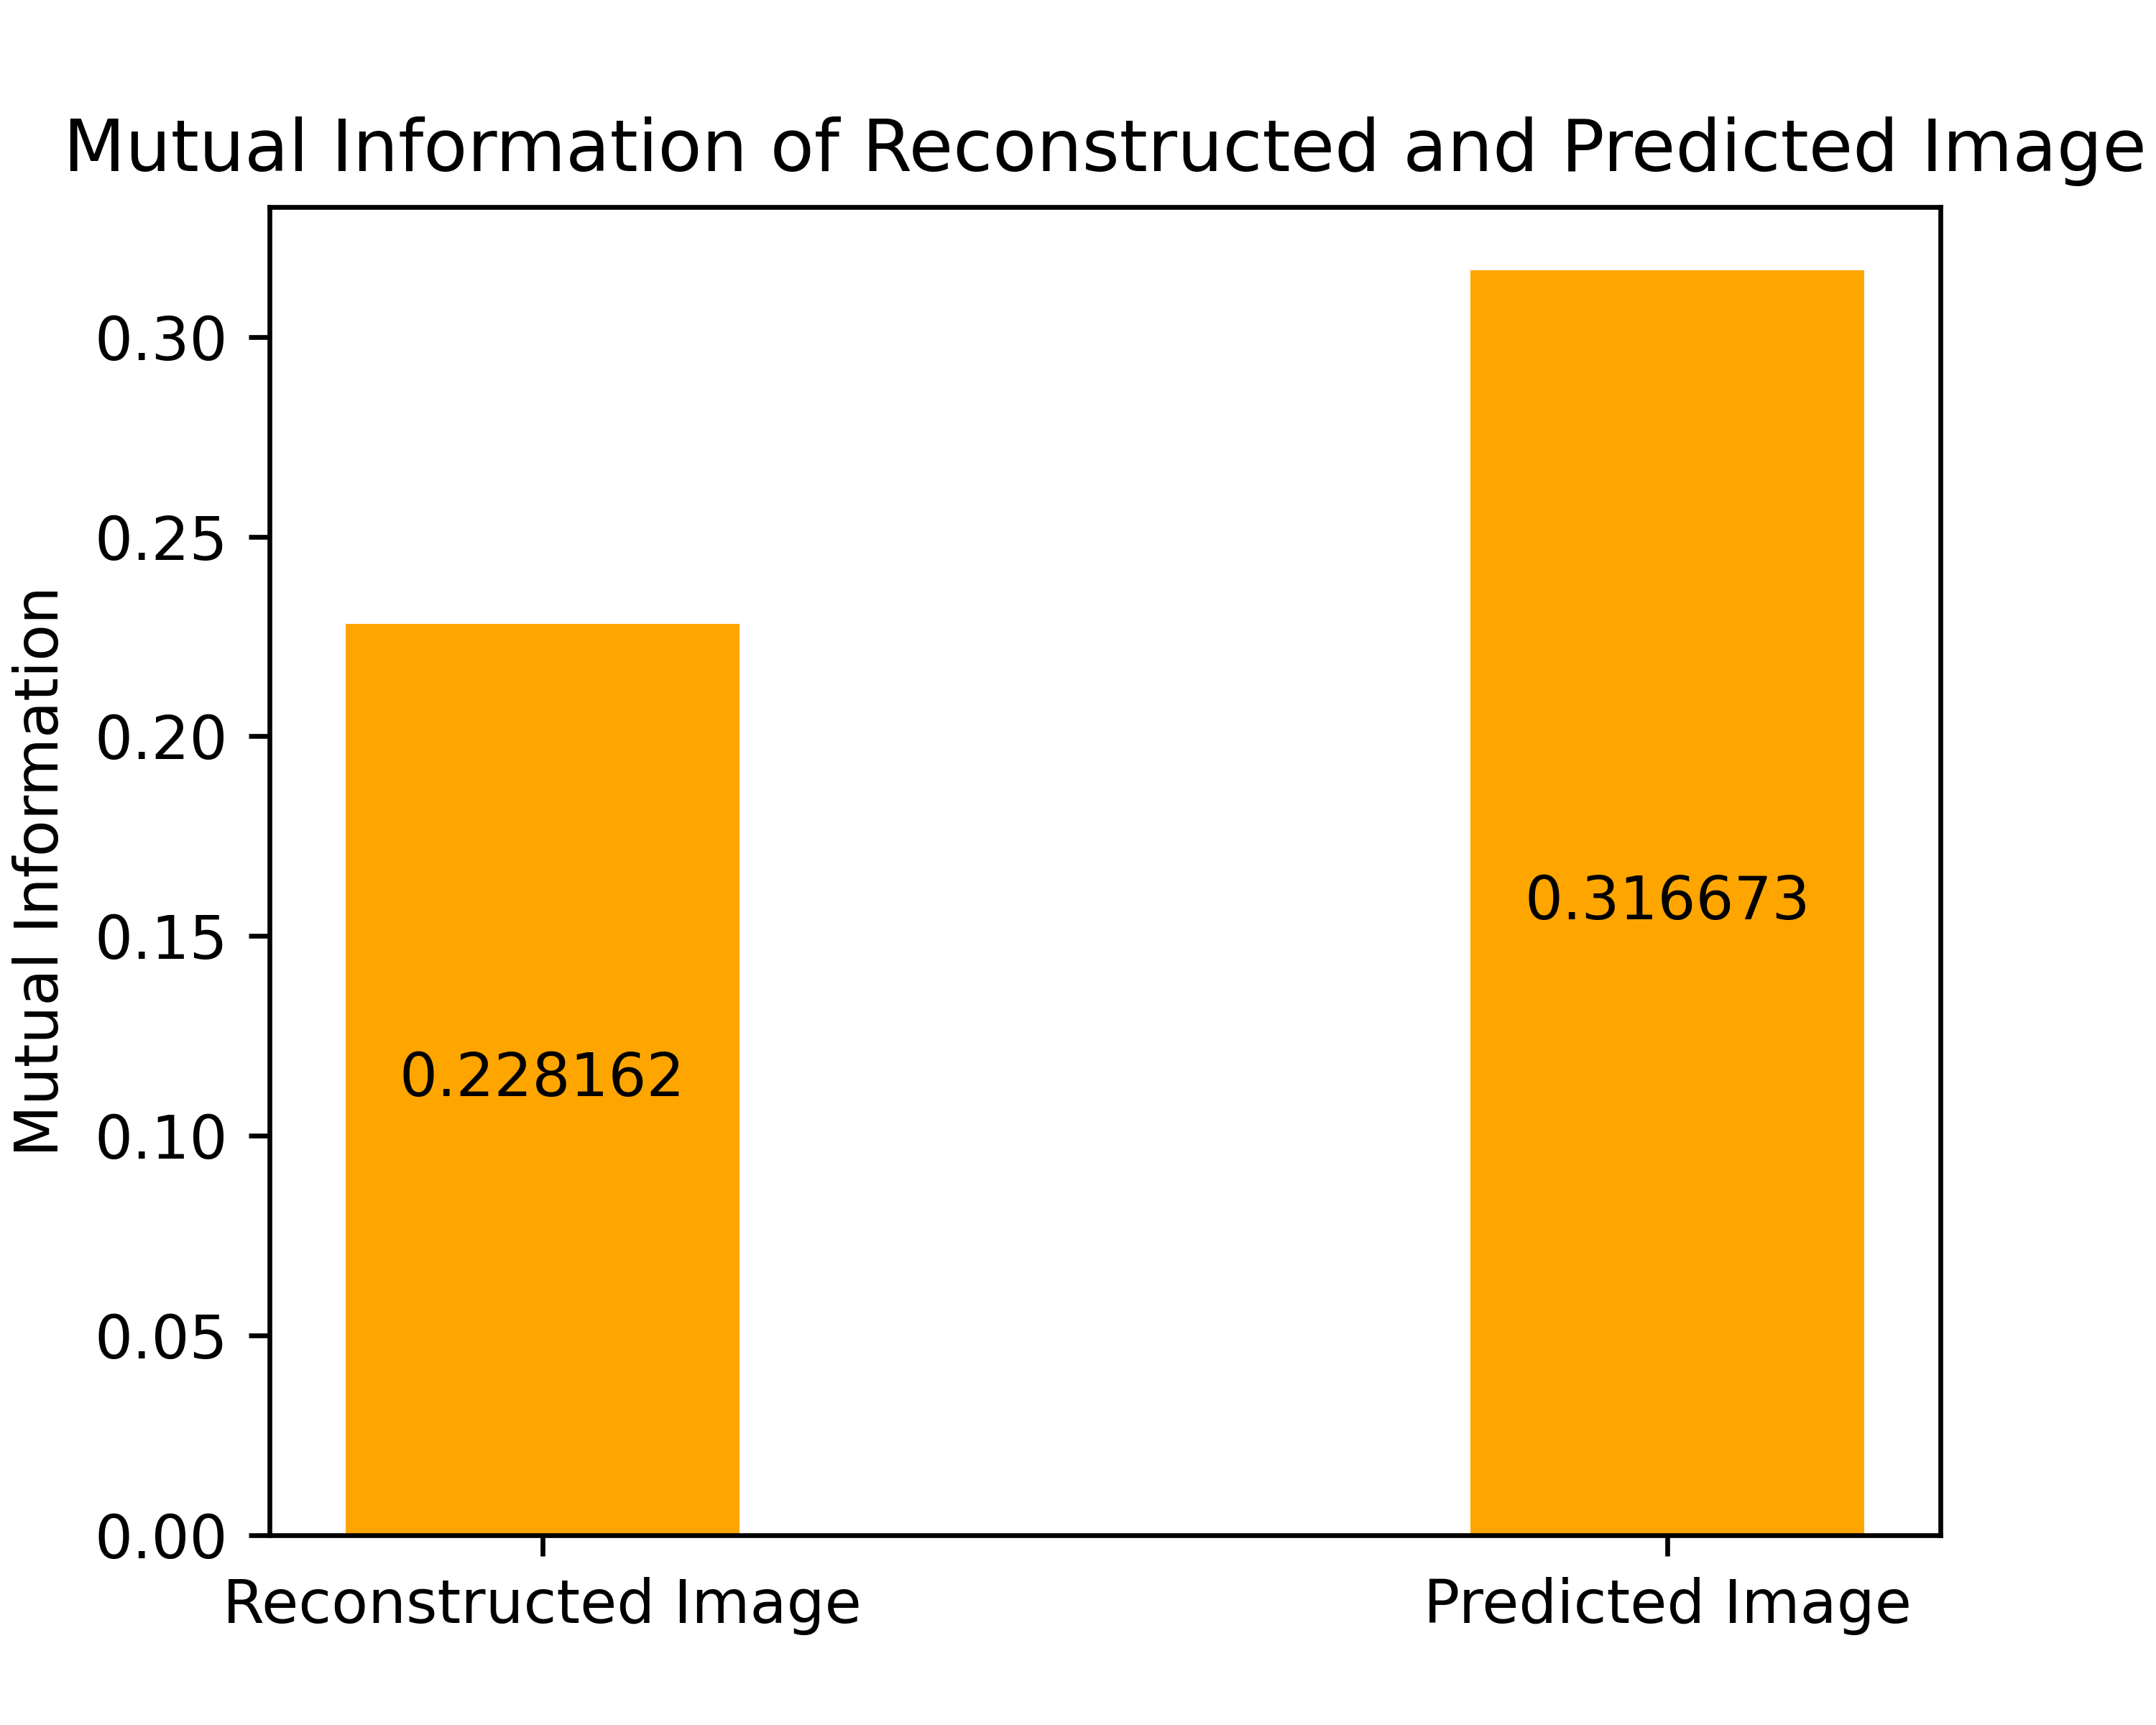
\includegraphics[width=0.75\columnwidth]{image/chap06/img611.png}
	\caption{测试集图像及其预测图象与原图像的NMI的均值}
	\label{fig611}
\end{figure}

从计算结果可知,预测图像与原图像之间的NMI值大于重建图像与原图像间的NMI值。其结果表明,预测图像比重建图像具有更高的相似性。

\section{模型评估总结}
对于验证集中的皮肤癌图片,我们计算出这1000张预测图像与原图像、重建图像与原图像的上述各评价指标的均值,记录如下表:

\begin{table}[h]
	\caption{验证集的各项评价指标的均值}
	\begin{tabular}{c|cccc}
		\hline
		& MSE                                                                                                                    & PSNR              & SSIM               & Cosine             \\ \hline
		\begin{tabular}[c]{@{}c@{}}Reconstructed\\ Image\end{tabular} & 274.263                                                                                                                & 24.6191           & 0.546436           & 0.934411           \\ \hline
		\begin{tabular}[c]{@{}c@{}}Predicted\\ Image\end{tabular}     & 126.677$\downarrow$                                                                                                    & 28.7648$\uparrow$ & 0.725969$\uparrow$ & 0.967805$\uparrow$ \\ \hline
		& Hash                                                                                                                   & Hist              & NMI                &                    \\ \hline
		\begin{tabular}[c]{@{}c@{}}Reconstructed\\ Image\end{tabular} & \begin{tabular}[c]{@{}c@{}}pHash:0.9015\\ aHash:0.911672\\ dHash:0.742875\end{tabular}                                 & 0.51264           & 0.228162           &                    \\ \hline
		\begin{tabular}[c]{@{}c@{}}Predicted\\ Image\end{tabular}     & \begin{tabular}[c]{@{}c@{}}pHash:0.949906$\uparrow$\\ aHash:0.951219$\uparrow$\\ dHash:0.842469$\uparrow$\end{tabular} & 0.73802$\uparrow$ & 0.316673$\uparrow$ &                    \\ \hline
	\end{tabular}
\end{table}


根据上述各指标的评估结果可知:训练出的神经网络模型的优化图像在逐像素比较的评估标准(MSE、PSNR、Hist)下均能取得相较重建图像更好的分辨率;且在结构相似度的评价指标SSIM下也具有更好的表现;在余弦相似度和哈希相似度等指标下也具有更高的相似度;在信息论的评价标准(NMI)下,预测图像相较于重建图像丢失更少的信息,具有更高的还原度。

因此,可以得出结论:Transformer模型在将低质量光声重建图像预测为高质量光声重建图像的优化任务上,具有较好的优化效果。将该模型应用于光声成像的后处理能显著改善采样信息丢失导致的成像精度低的问题,为低成本下获取高精度光声图像的研究提供了一个解决方法。

\section{模型不足与发展方向}
	\begin{itemize}
	\item [1)]由于项目实施的时间有限,数据集的图片数量和丰富程度还不够充实。在今后的优化中,可以适当增加数据集的来源,或通过在光声成像的仿真及重建中设置不同的传感器数量等方式来获取更丰富的数据集。
	\item [2)]由于训练次数有限,该模型在优化50个传感器下的重建图像上效果显著;而在优化100、200、400个传感器下的重建图像的效果并不是很好。这点可以通过增加由100、200、400个传感器得出的重建图像的数据集及增加训练epoch次数等方式解决。
	\item [3)]在医学的运用过程中,模型的推理成本也是一项很重要的指标。在今后的优化中,可以通过量化、剪枝\cite{rao2021dynamicvit}、知识蒸馏\cite{touvron2021training} \cite{wu2022tinyvit}、参数共享\cite{zhang2022minivit}等方法减少内存消耗与提高模型运行速度。
\end{itemize}
\newclearpage

% 结语

% 附录部分
\backmatter
% 参考文献. 因不需要纳入章节目录, 故放入附录部分
% 实际上参考文献是属于论文主体部分
\makereferences

% 附录
% {
% \appendix
% \chapter{附录}



% \newclearpage
% }

%%
% 致谢
% 谢辞应以简短的文字对课题研究与论文撰写过程中曾直接给予帮助的人员(例如指导教师、答疑教师及其他人员)表示对自己的谢意,这不仅是一种礼貌,也是对他人劳动的尊重,是治学者应当遵循的学术规范。内容限一页。
% modifier: 黄俊杰
% update date: 2017-04-15
%%

\chapter{致谢}

首先我要感谢论文的指导老师时聪教授。在课题立项初期,我对当今的学术热点了解不深,时聪老师以其对整个研究领域的深刻理解和敏锐的洞察力给了我针对性的指导,帮助我完成了课题的选择及研究方向的确定。在项目实践的过程中,由于匮乏独自完成课题研究所需的经验,我常常请教时聪老师,在解决一项项学术问题的过程中,我不断提高着分析和解决问题的能力与养成了一定的科学素养,这使我在项目研究后期能开始独立完成课题的研究工作。这段经历的收获不在于学习到了多少具体的专业知识,而在于培养了我的科研思维和坚定了我选择学术研究道路的决心。

其次我还要感谢我本科的老师们,在此我郑重附上他们的名字:叶小平教授,刘长剑教授,陈秀卿教授,易泰山教授,赵育林教授,李铎教授,刘海峰教授,邵国宽教授,杨燕教授,魏国栋教授。他们不仅教会了我相关的专业知识,还培养了我数学的思维方式。

最后,我还要感谢我的家人,如果没有他们在背后的付出和支持,我就无法取得现在的成果。

\vskip 108pt
\begin{flushright}
	黄梓航\makebox[1cm]{} \\
	\today
\end{flushright}

    % 致谢
\newclearpage

% \makeGrade      % 成绩评定记录表
\end{document}

